\documentclass[compress]{beamer}
\usepackage{ifthen,verbatim}

\newcommand{\isnote}{}
\xdefinecolor{lightyellow}{rgb}{1.,1.,0.25}
\xdefinecolor{darkblue}{rgb}{0.1,0.1,0.7}

%% Uncomment this to get annotations
%% \def\notes{\addtocounter{page}{-1}
%%            \renewcommand{\isnote}{*}
%% 	   \beamertemplateshadingbackground{lightyellow}{white}
%%            \begin{frame}
%%            \frametitle{Notes for the previous page (page \insertpagenumber)}
%%            \itemize}
%% \def\endnotes{\enditemize
%% 	      \end{frame}
%%               \beamertemplateshadingbackground{white}{white}
%%               \renewcommand{\isnote}{}}

%% Uncomment this to not get annotations
\def\notes{\comment}
\def\endnotes{\endcomment}

\setbeamertemplate{navigation symbols}{}
\setbeamertemplate{headline}{\mbox{ } \hfill
\begin{minipage}{5.5 cm}
\vspace{-0.75 cm} \small
\end{minipage} \hfill
\begin{minipage}{4.5 cm}
\vspace{-0.75 cm} \small
\begin{flushright}
\ifthenelse{\equal{\insertpagenumber}{1}}{}{Jim Pivarski \hspace{0.2 cm} \insertpagenumber\isnote/\pageref{numpages}}
\end{flushright}
\end{minipage}\mbox{\hspace{0.2 cm}}\includegraphics[height=1 cm]{../cmslogo} \hspace{0.1 cm} \includegraphics[height=1 cm]{../tamulogo} \hspace{0.01 cm} \vspace{-1.05 cm}}

\begin{document}
\begin{frame}
\vfill
\begin{center}
\textcolor{darkblue}{\Large Track-based endcap alignment}

\vfill
\begin{columns}
\column{0.3\linewidth}
\begin{center}
\large
\textcolor{darkblue}{\it Jim Pivarski}

Aysen Tatarinov

Vadim Khotilovich

Alexei Safonov
\end{center}
\end{columns}

\begin{columns}
\column{0.3\linewidth}
\begin{center}
\scriptsize
{\it Texas A\&M University}
\end{center}
\end{columns}

\vfill
14 May, 2010

\end{center}
\end{frame}

%% \begin{notes}
%% \item This is the annotated version of my talk.
%% \item If you want the version that I am presenting, download the one
%% labeled ``slides'' on Indico (or just ignore these yellow pages).
%% \item The annotated version is provided for extra detail and a written
%% record of comments that I intend to make orally.
%% \item Yellow notes refer to the content on the {\it previous} page.
%% \item All other slides are identical for the two versions.
%% \end{notes}

\small

\begin{frame}
\frametitle{Construction of geometry}
\begin{enumerate}
\item Photogrammetry: $x$, $y$, $z$, $\phi_x$ (some of which are bigger than 2~mrad), $\phi_z$
\item Disk-bending from hardware: additional correction on $\phi_x$ and ring radii
\item Small additional-additional correction on ring radii to set closure = 0
\item Beam-halo $+$ PG $x$, $\phi_z$ at the level of {\it disks}
\item globalMuon {\it disk}-alignment in global $x$, $y$, $\phi_z$ (future)
\item final global $z$ corrections for {\it disks?} (future)
\end{enumerate}

%% \begin{itemize}\setlength{\itemsep}{0.5 cm}
%% \item 
%% \end{itemize}
%% \hspace{-0.83 cm} \textcolor{darkblue}{\Large Outline2}
\end{frame}

\begin{frame}
\frametitle{Disk-bending}
\begin{itemize}
\item Applied in the right direction (bottoms of chambers go toward I.P.
\item But photogrammetry spread in values is larger than this change

\item The numbers (rad):
\begin{tabular}{c c | c c}
ME$+$1/1 & 0.002 & ME$-$1/1 & 0.002 \\
ME$+$1/2 & 0.002 & ME$-$1/2 & 0.002 \\
ME$+$1/3 & 0.002 & ME$-$1/3 & 0.002 \\
ME$+$2/1 & 0.00239 & ME$-$2/1 & 0.00261 \\
ME$+$2/2 & 0.00273 & ME$-$2/2 & 0.00303 \\
ME$+$3/1 & 0.00230 & ME$-$3/1 & 0.00237 \\
ME$+$3/2 & 0.00263 & ME$-$3/2 & 0.00288 \\
ME$+$4/1 & 0.00208 & ME$-$4/1 & 0.00221 \\
ME$+$4/2 & 0.002 & ME$-$4/2 & 0.002 \\
\end{tabular}

\item The 3-sig-fig numbers are from Oleg
\item The ``0.002'' are an approximation for the rest
\item Ring-radius corrections $= (\phi_x) \times \mbox{\scriptsize (dist from chamber center to disk center)\hspace{-1 cm}}$
\begin{itemize}
\item ``disk center'' rather than ``disk surface'' is an update that
  significantly improves hardware/track ring-radius agreement (the
  missing factor of 2)
\end{itemize}
\end{itemize}
\end{frame}

\begin{frame}
\frametitle{Ring radii from tracks}

\begin{itemize}
\item After the expected correction from disk-bending geometry, we
  apply another ring-radius correction to make beam-halo closure zero

\begin{tabular}{c c c}
Ring & radius change & closure/chamber (before) \\\hline
ME$+$1/1 & $-$0.64 mm & $-$0.11 mm \\
ME$+$1/2 & $+$0.60 mm & $+$0.10 mm \\
ME$+$2/1 & $+$0.37 mm & $+$0.13 mm \\
ME$+$2/2 & $-$1.75 mm & $-$0.31 mm \\
ME$+$3/1 & $+$0.33 mm & $+$0.12 mm \\
ME$+$3/2 & $-$1.52 mm & $-$0.27 mm \\
ME$+$4/1 & $-$0.53 mm & $-$0.19 mm \\\hline
ME$-$1/1 & $-$1.54 mm & $-$0.27 mm \\
ME$-$1/2 & $+$0.11 mm & $+$0.02 mm \\
ME$-$2/1 & $+$0.04 mm & $+$0.01 mm \\
ME$-$2/2 & $-$0.79 mm & $-$0.14 mm \\
ME$-$3/1 & $-$0.11 mm & $-$0.04 mm \\
ME$-$3/2 & $-$1.56 mm & $-$0.27 mm \\
ME$-$4/1 & $-$0.55 mm & $-$0.19 mm \\
\end{tabular}

\item Signs are ``radius$-$after minus radius$-$before''

\item The ME2/2, 3/2 rings get the largest additional correction
\end{itemize}
\end{frame}

\begin{frame}
\frametitle{Beam-halo results}

\begin{itemize}
\item Beam-halo alignment was applied to {\it disks,} rather than
  rings, so that the globalMuon alignment can combine statistics
\begin{itemize}
\item cosmic ray globalMuons are much more precise for outer rings than inner rings
\end{itemize}
\item There were nine separate fits:
\begin{description}
\item[ME$+$1/1:] beam-halo only, disconnected segments between missing data
\item[ME$-$1/1:] same
\item[YE$+$1:] ME$+$1/2 and ME$+$1/3, PG in both, beam-halo only in ME$+$1/2
\item[YE$-$1:] same
\item[YE$+$2:] stations 2 and 2, PG in both, beam-halo in both
\item[YE$-$2:] same
\item[ME$+$4/1:] PG and beam-halo
\item[ME$-$4/1:] same
\item[ME$+$4/2:] beam-halo only alignment of 5 chambers
\end{description}

\item Aligned in 6 iterations: (1) $r\phi$, (2) $\phi_z$, (3) $r\phi$, (4) $\phi_z$, (5) $r\phi$, (6) $\phi_z$
\end{itemize}
\end{frame}

\begin{frame}
\frametitle{ME$+$1/1 $r\phi$}

\only<1>{Convergence in $r\phi$ positions

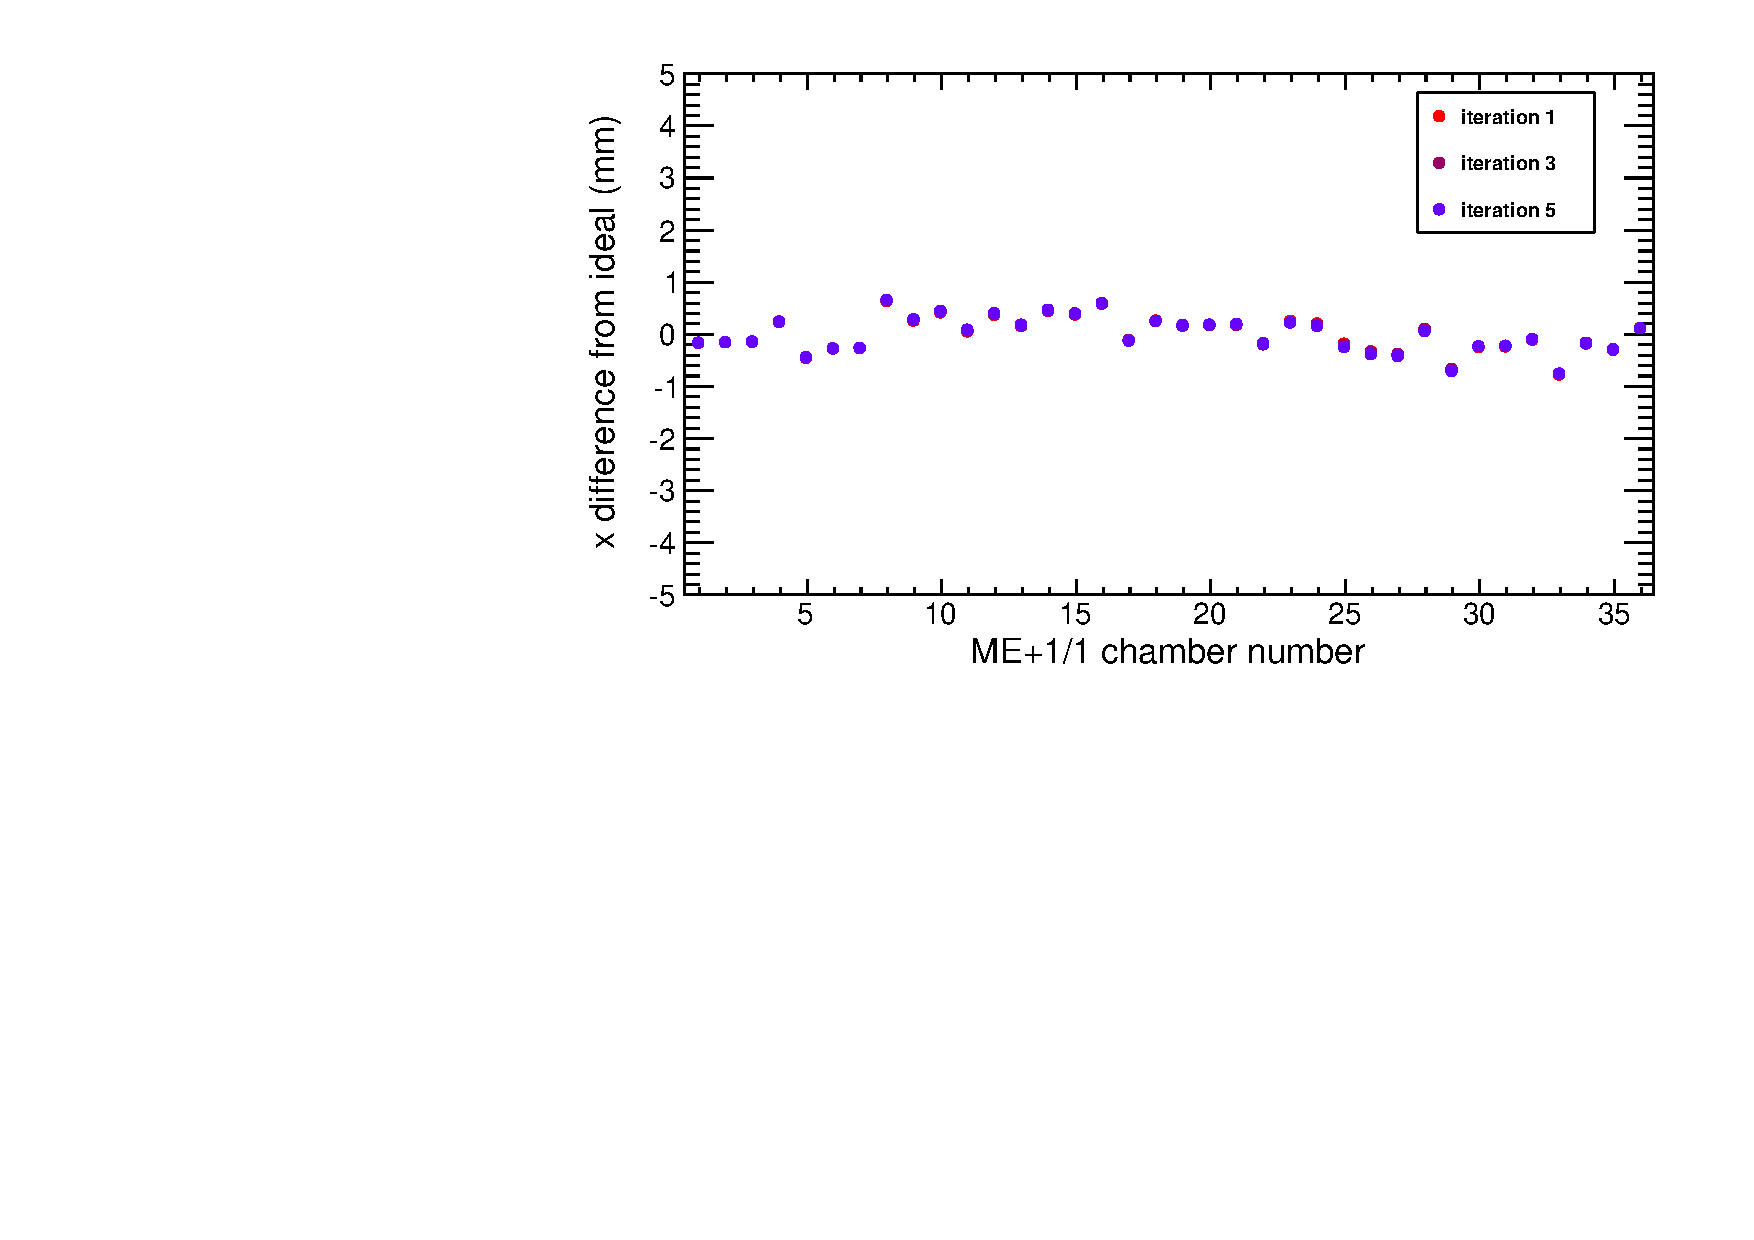
\includegraphics[width=\linewidth]{newplots_convergence_mep11_x.pdf}}
\only<2>{Fit residuals in $r\phi$ (not track residuals): no PG, perfect BH fit

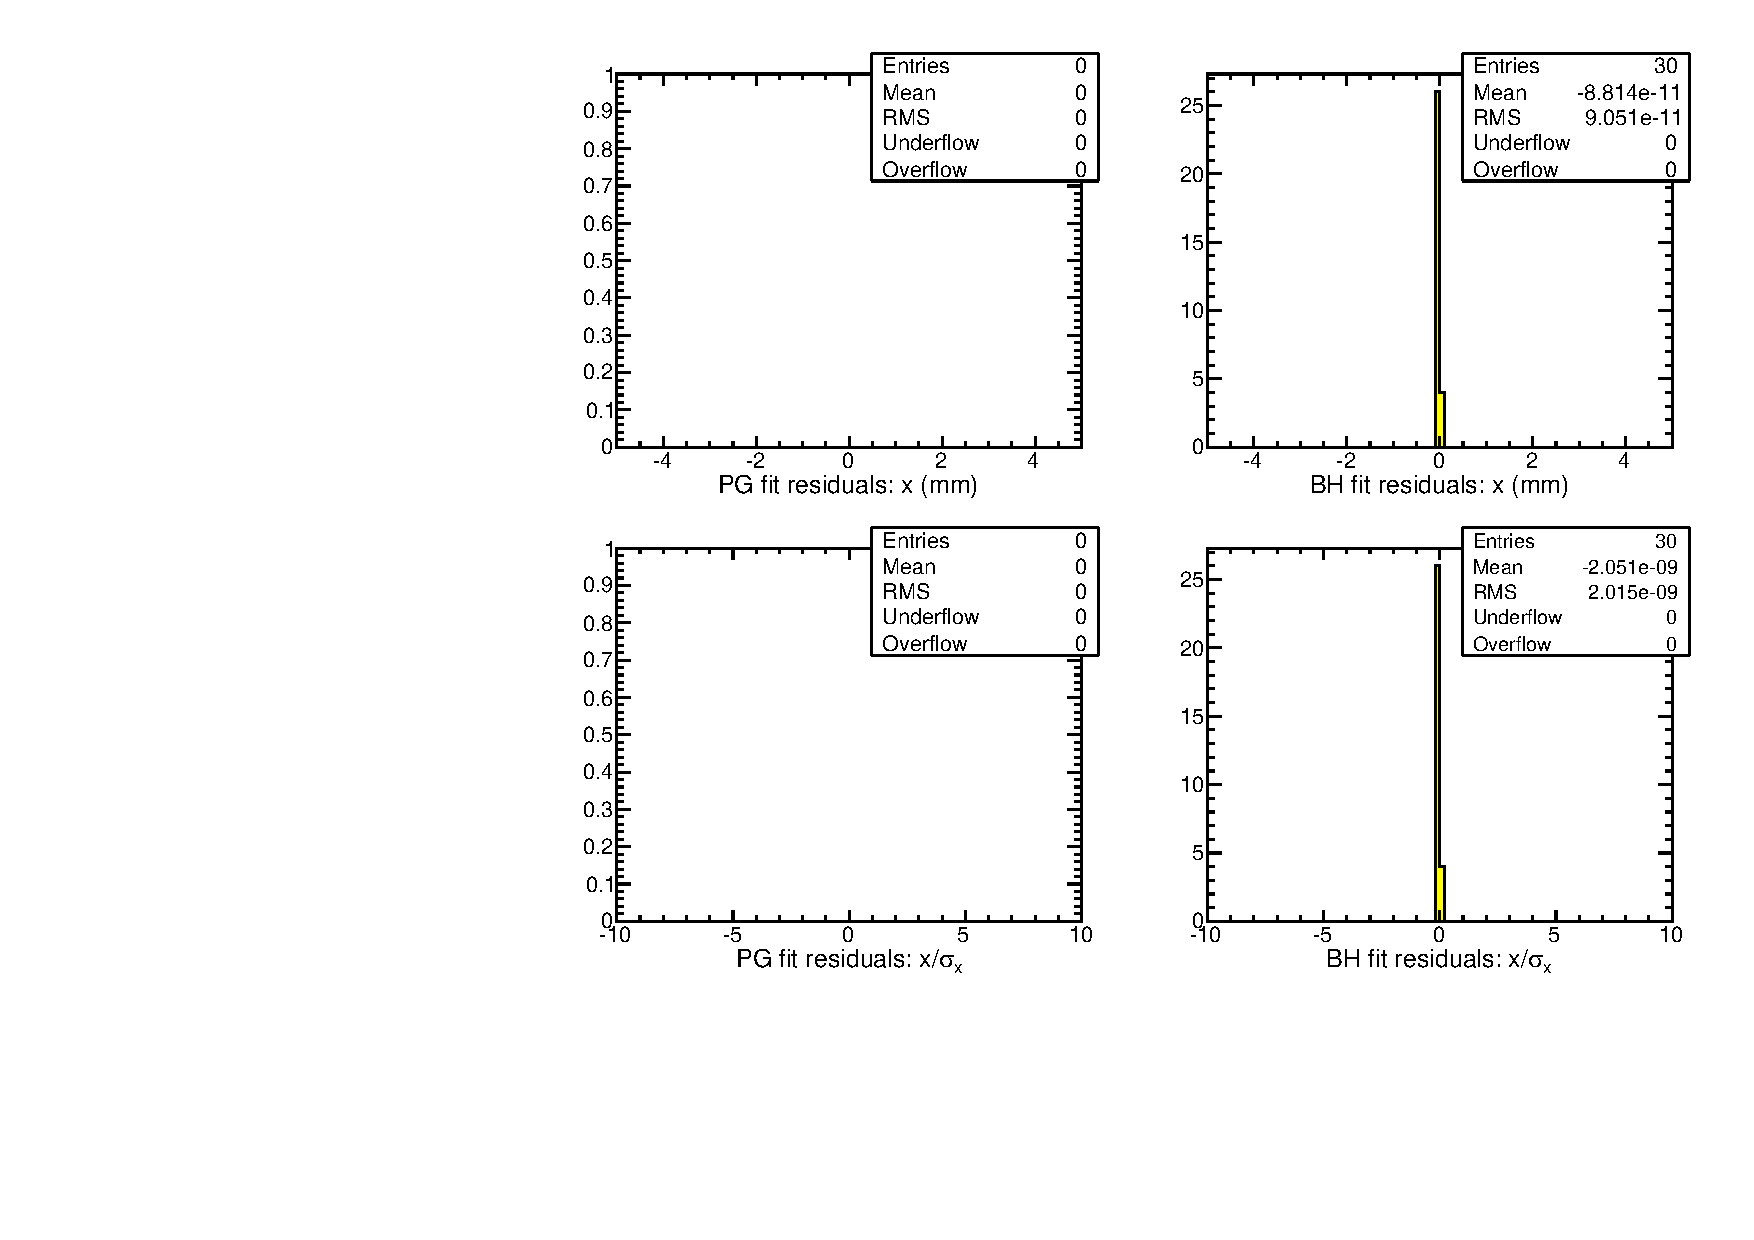
\includegraphics[width=0.9\linewidth]{newplots_fitresiduals_MEp1_1_x.pdf}}
\only<3>{Numbers in boxes are $\phi$ position uncertainty in each mode in rad

First 6 are completely undetermined (uncertainty is meaningless)

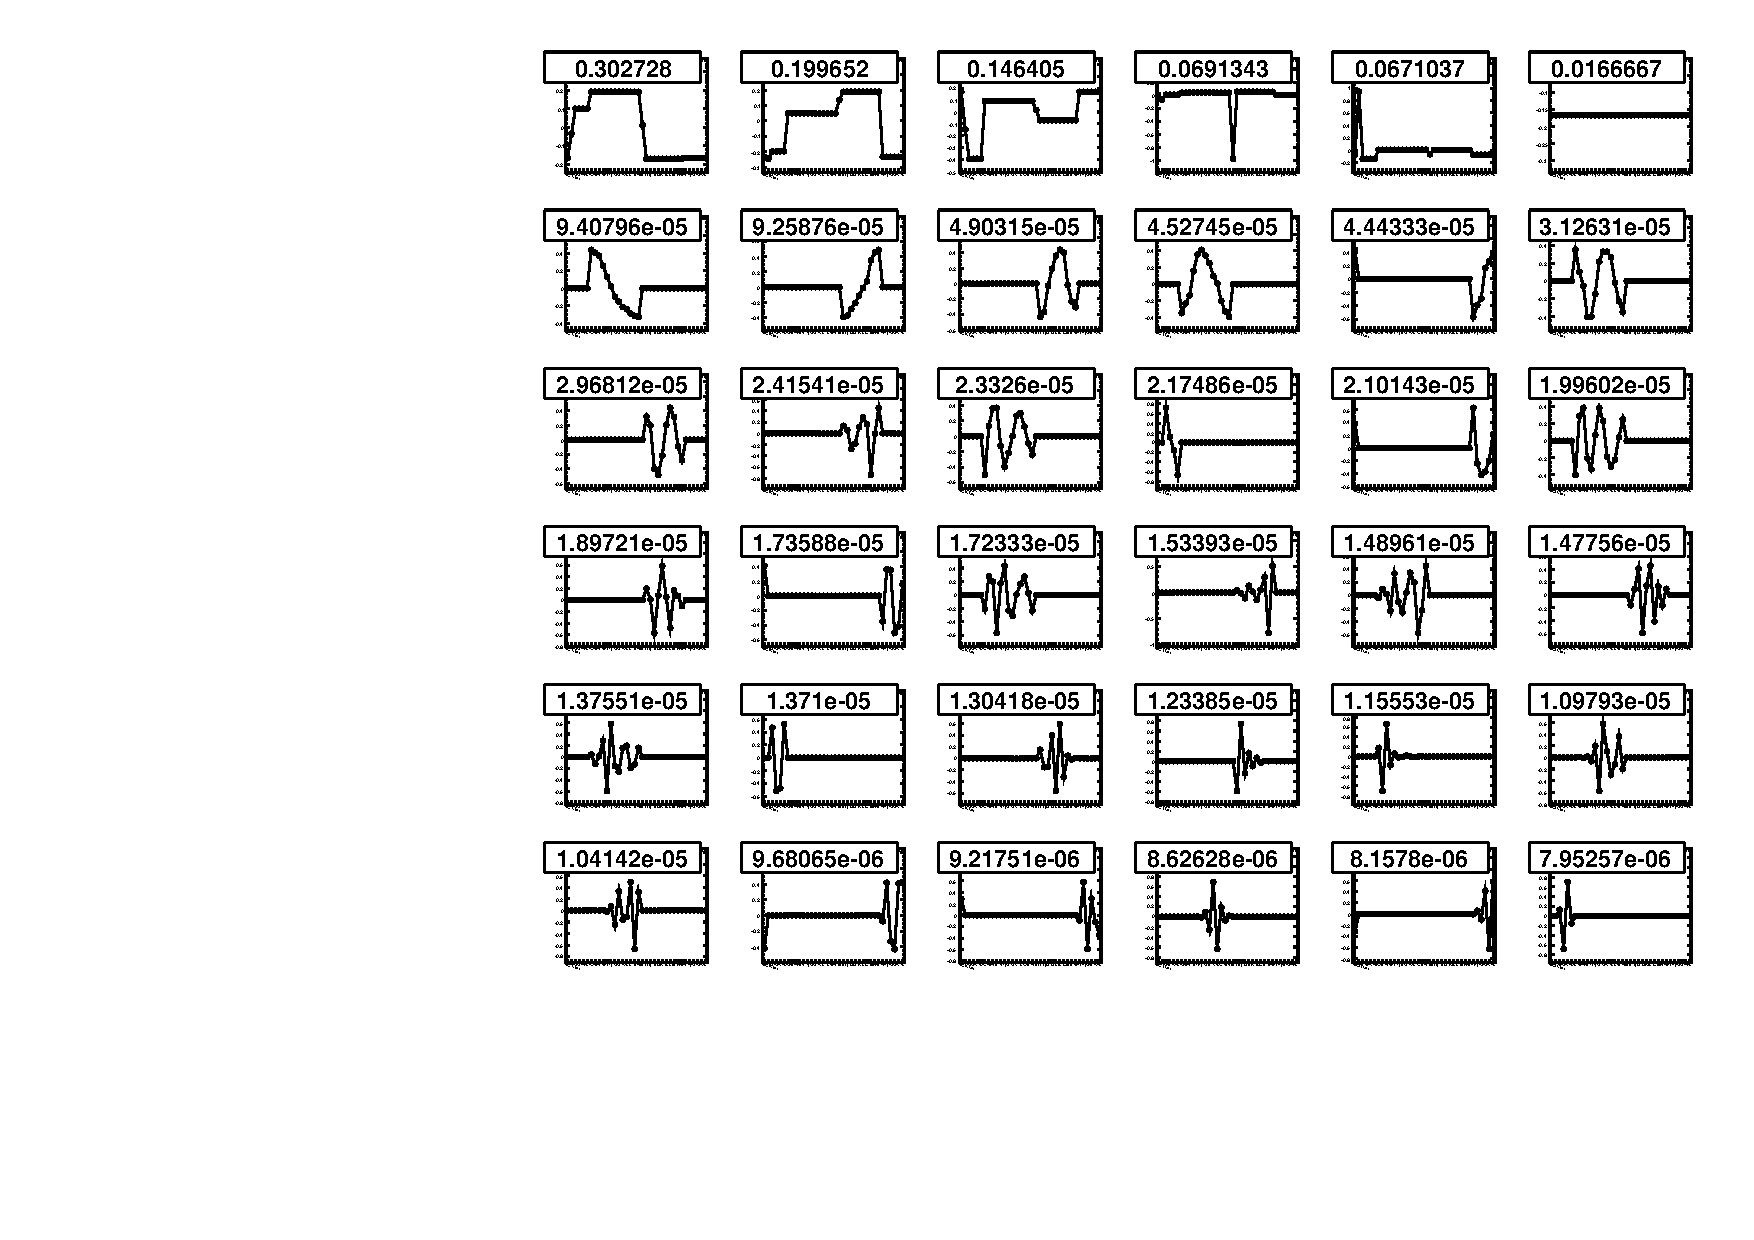
\includegraphics[width=0.9\linewidth]{newplots_errors_MEp1_1_x.pdf}}
\end{frame}

\begin{frame}
\frametitle{ME$+$1/1 $\phi_z$}

\only<1>{Convergence in $\phi_z$ angles

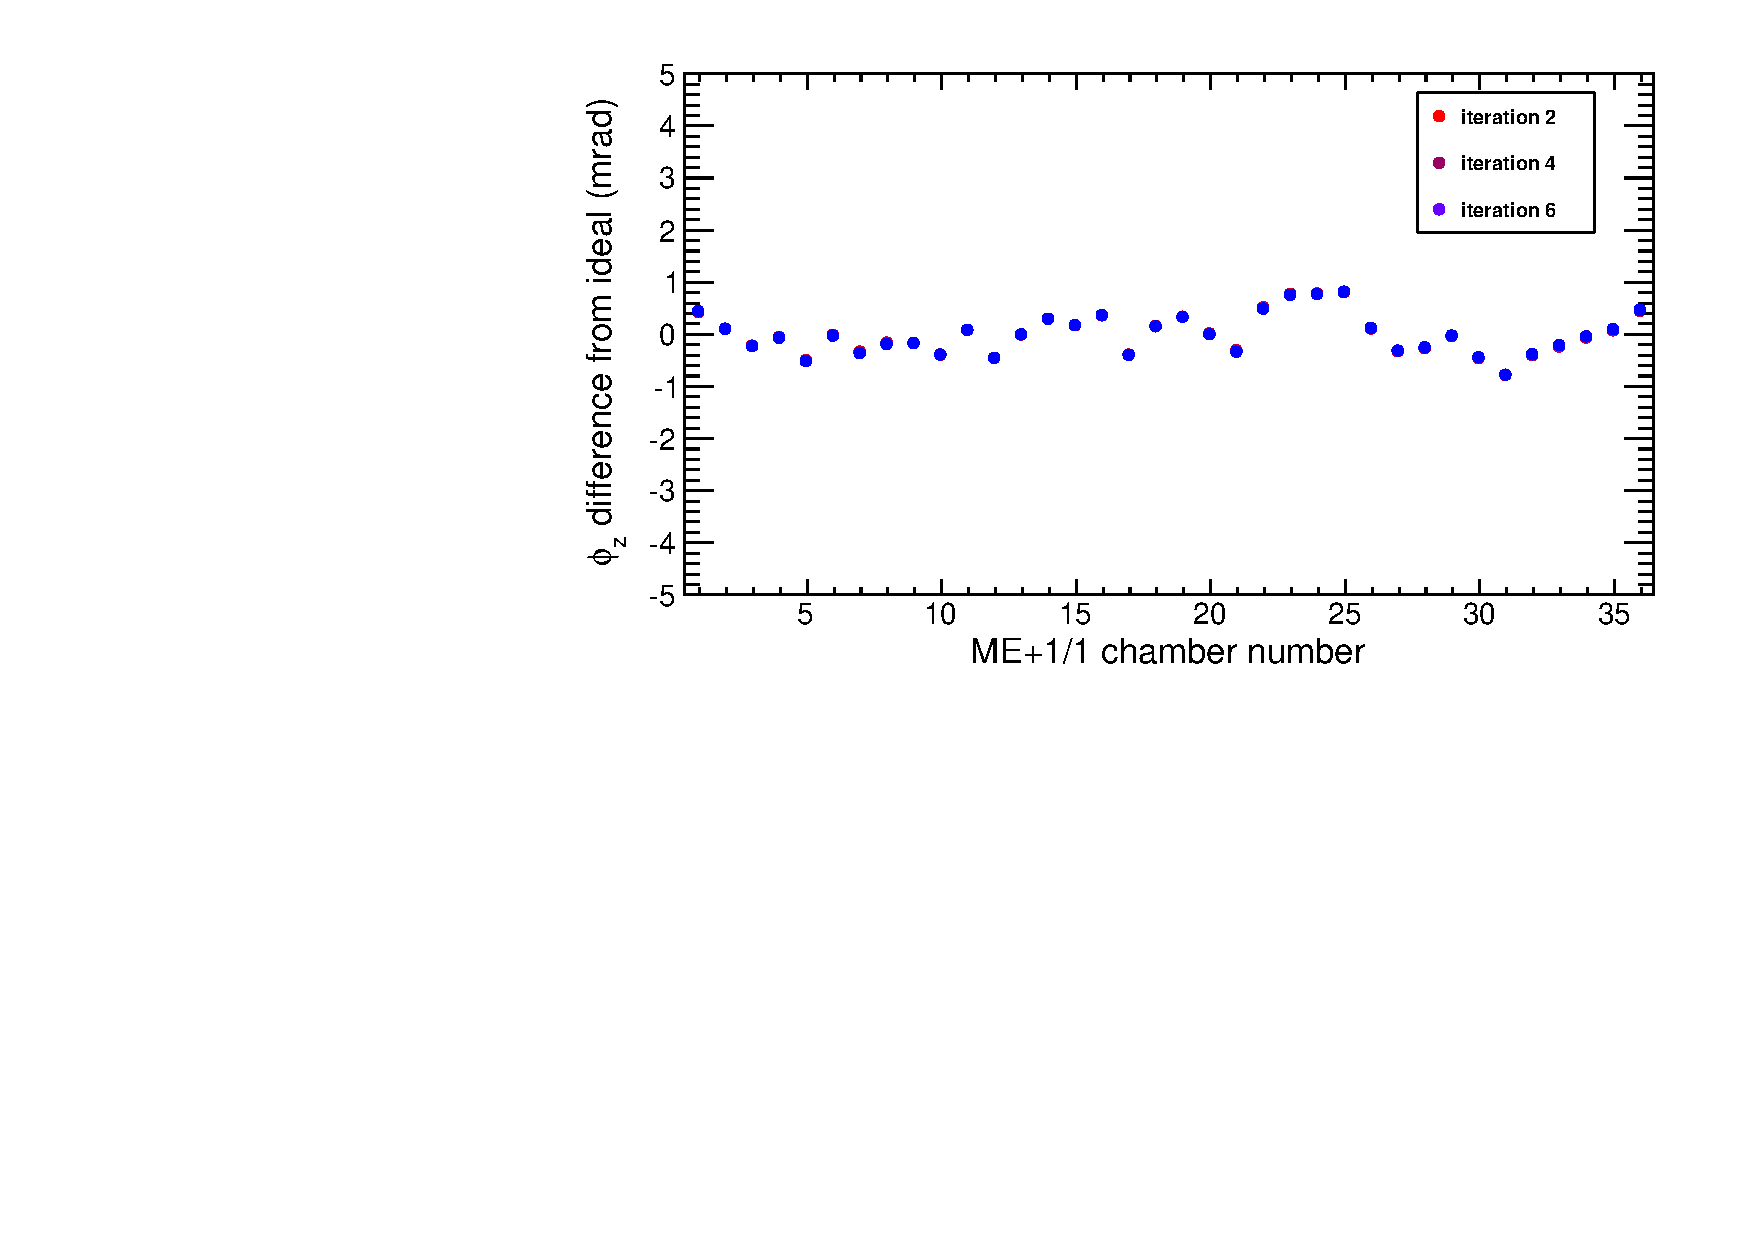
\includegraphics[width=\linewidth]{newplots_convergence_mep11_phiz.pdf}}
\only<2>{Fit residuals in $\phi_z$ (not track residuals): no PG, perfect BH fit

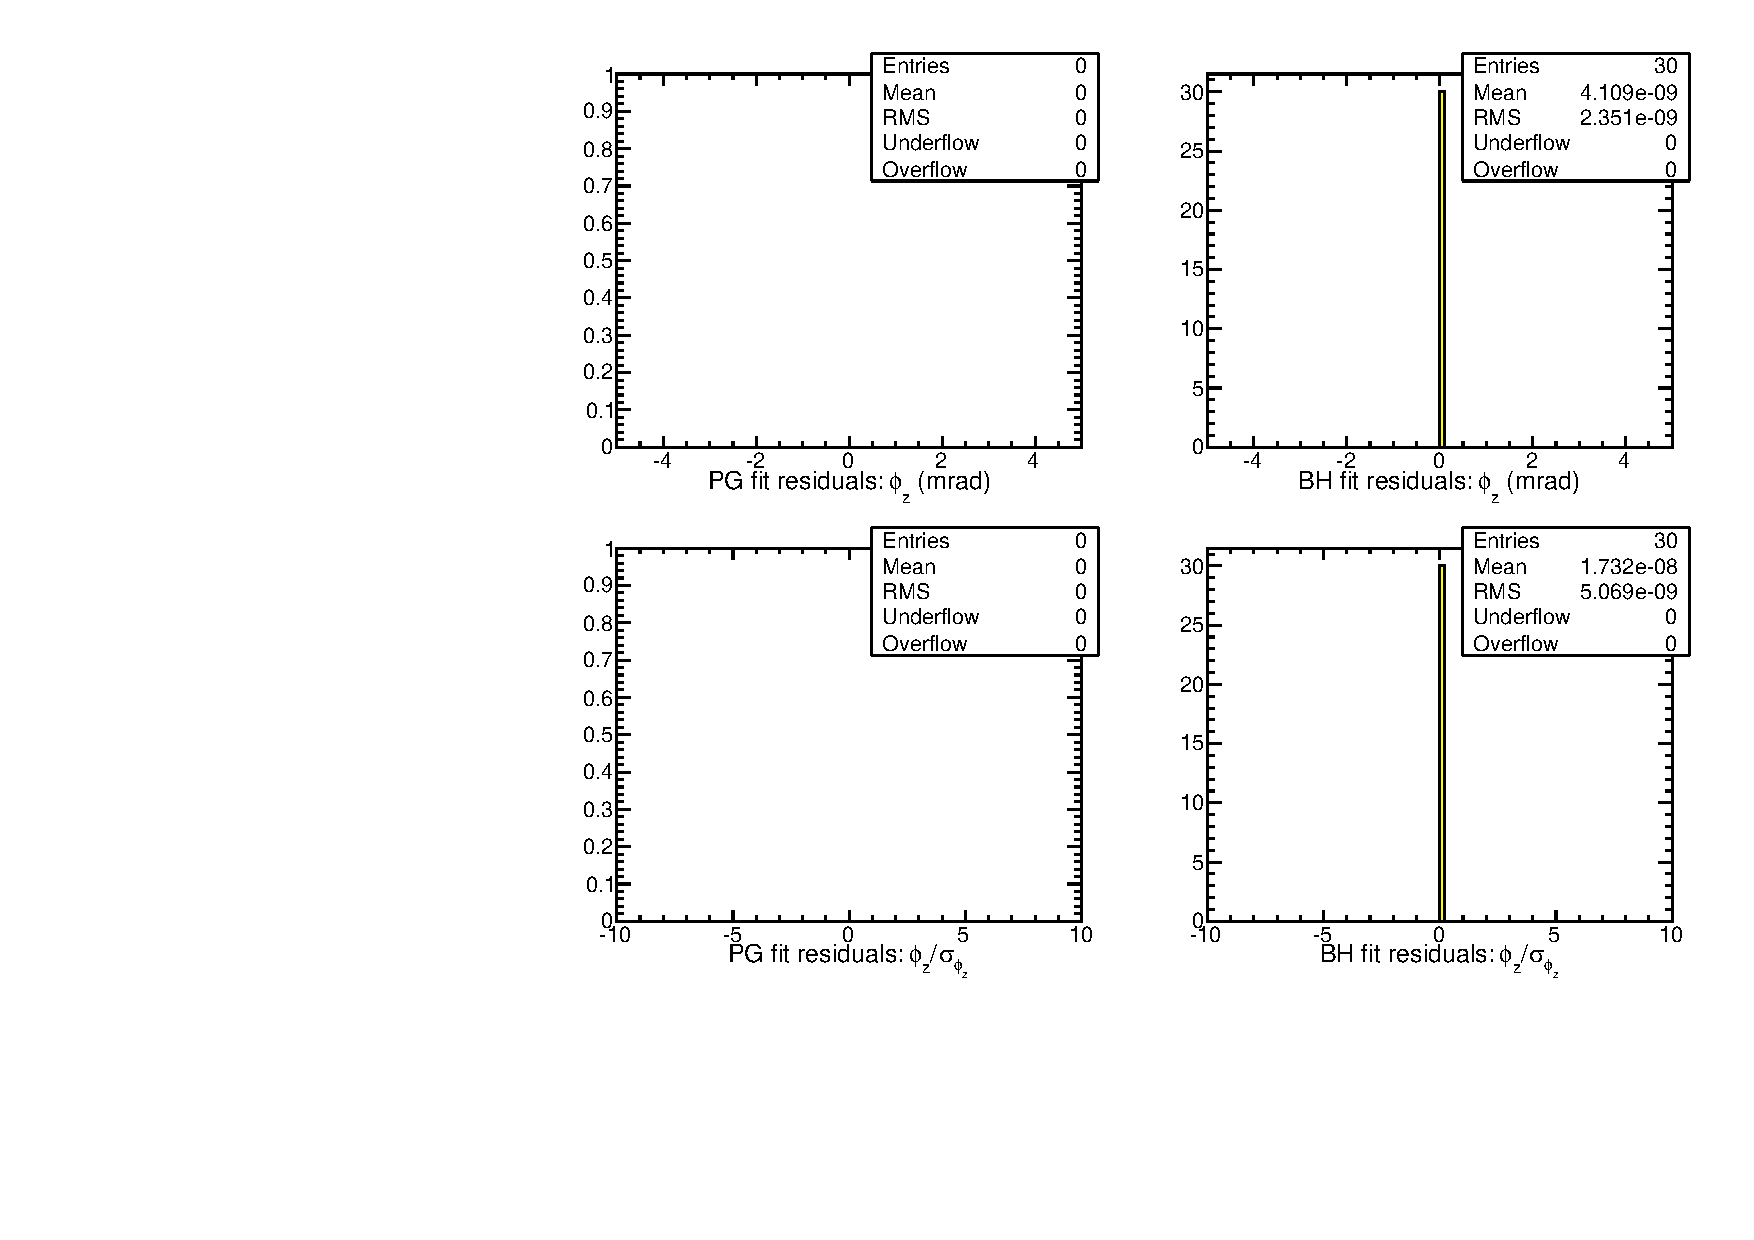
\includegraphics[width=0.9\linewidth]{newplots_fitresiduals_MEp1_1_phiz.pdf}}
\only<3>{Numbers in boxes are $\phi_z$ angle uncertainty in each mode in rad

First 6 are completely undetermined (uncertainty is meaningless)

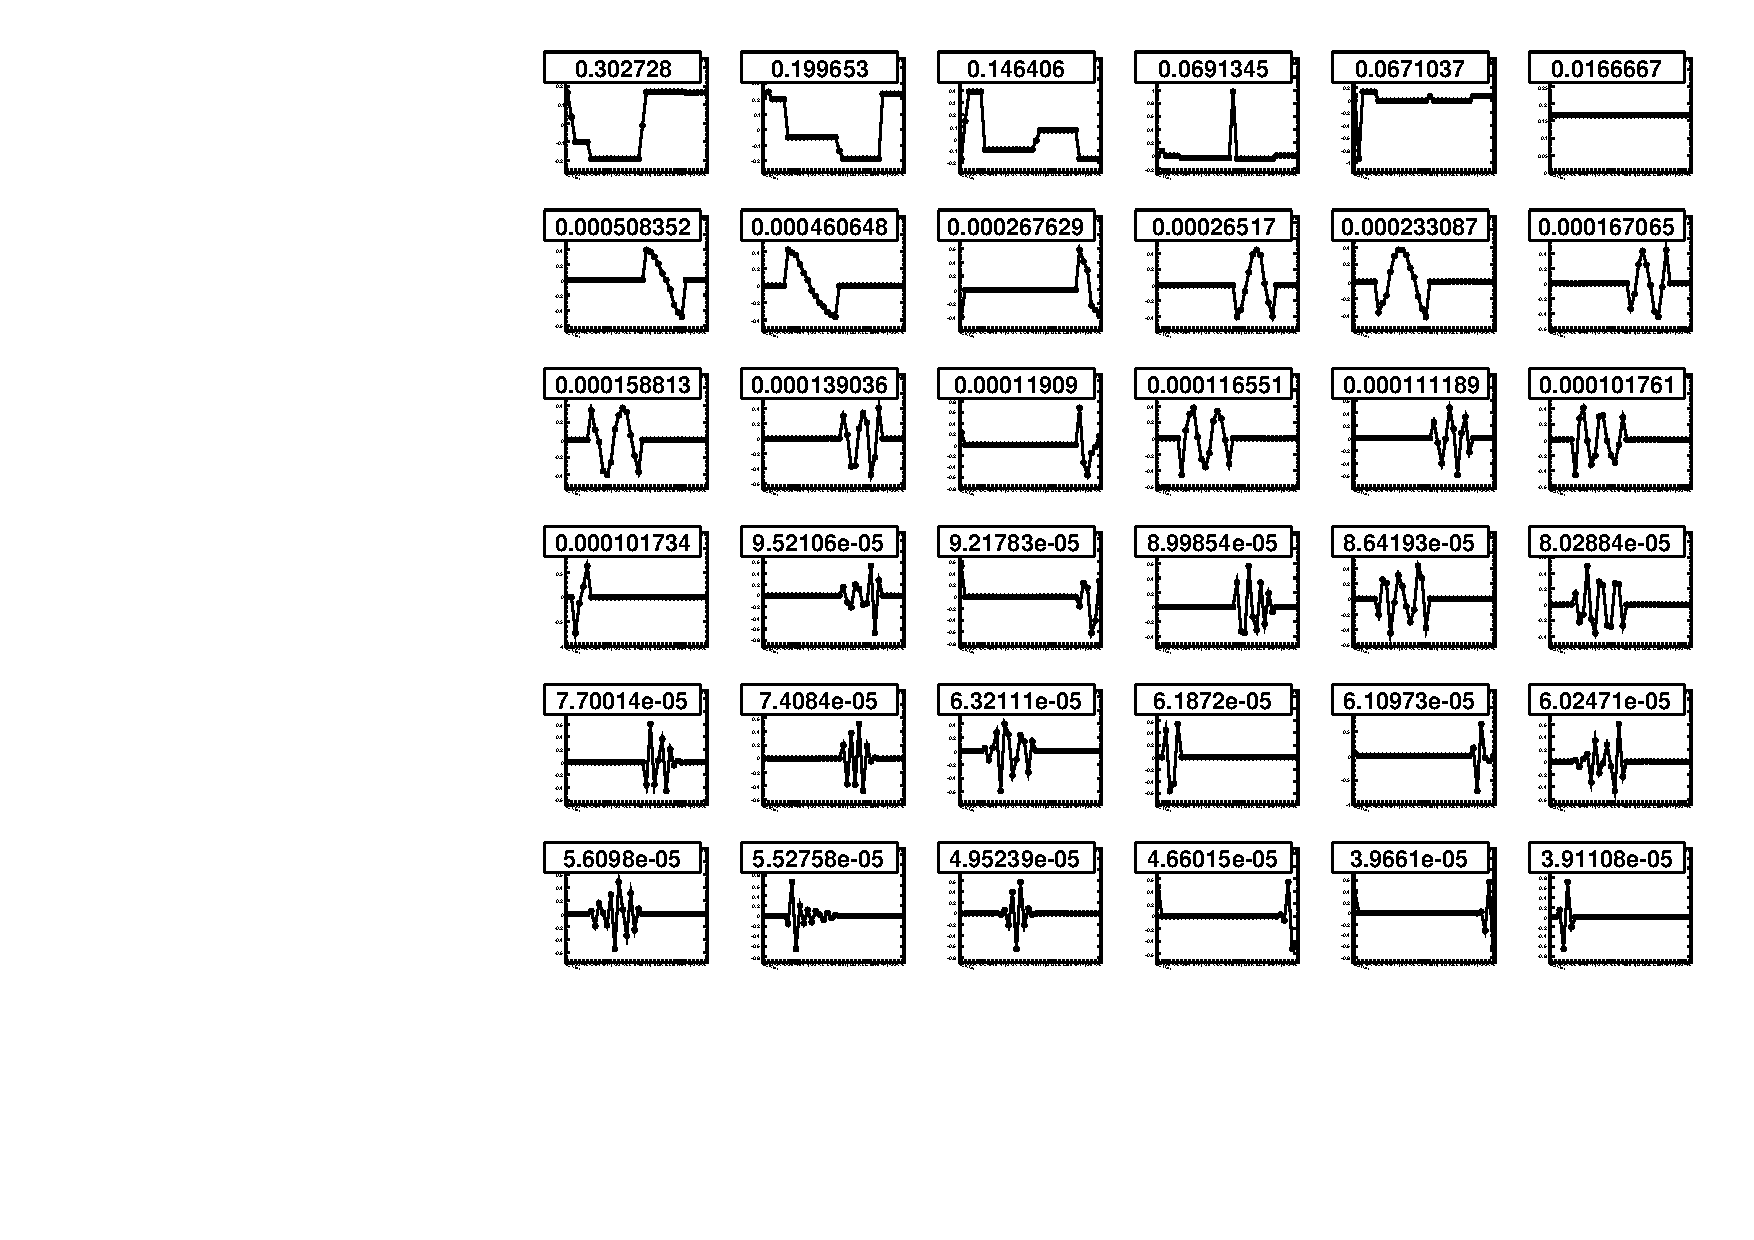
\includegraphics[width=0.9\linewidth]{newplots_errors_MEp1_1_phiz.pdf}}
\end{frame}

\begin{frame}
\frametitle{ME$-$1/1 $r\phi$}

\only<1>{Convergence in $r\phi$ positions

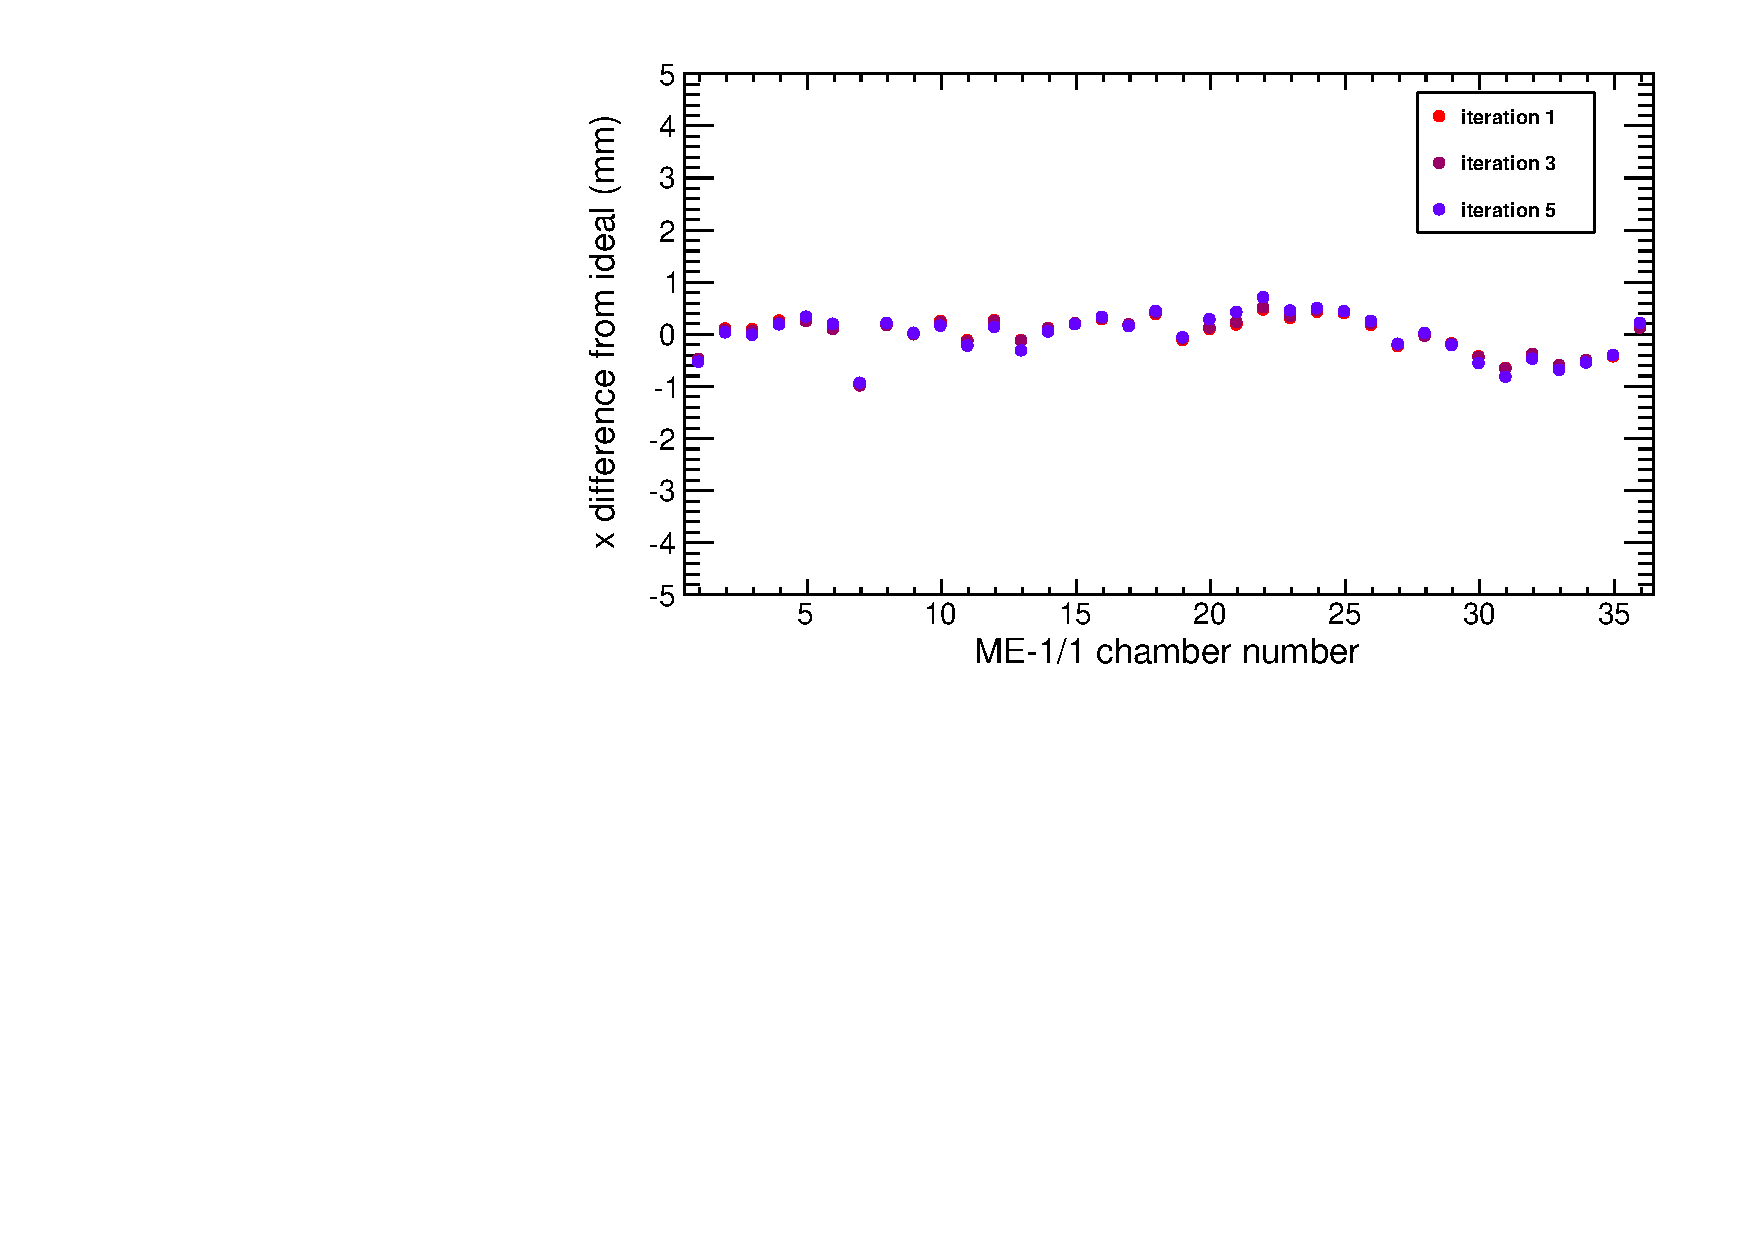
\includegraphics[width=\linewidth]{newplots_convergence_mem11_x.pdf}}
\only<2>{Fit residuals in $r\phi$ (not track residuals): no PG, perfect BH fit

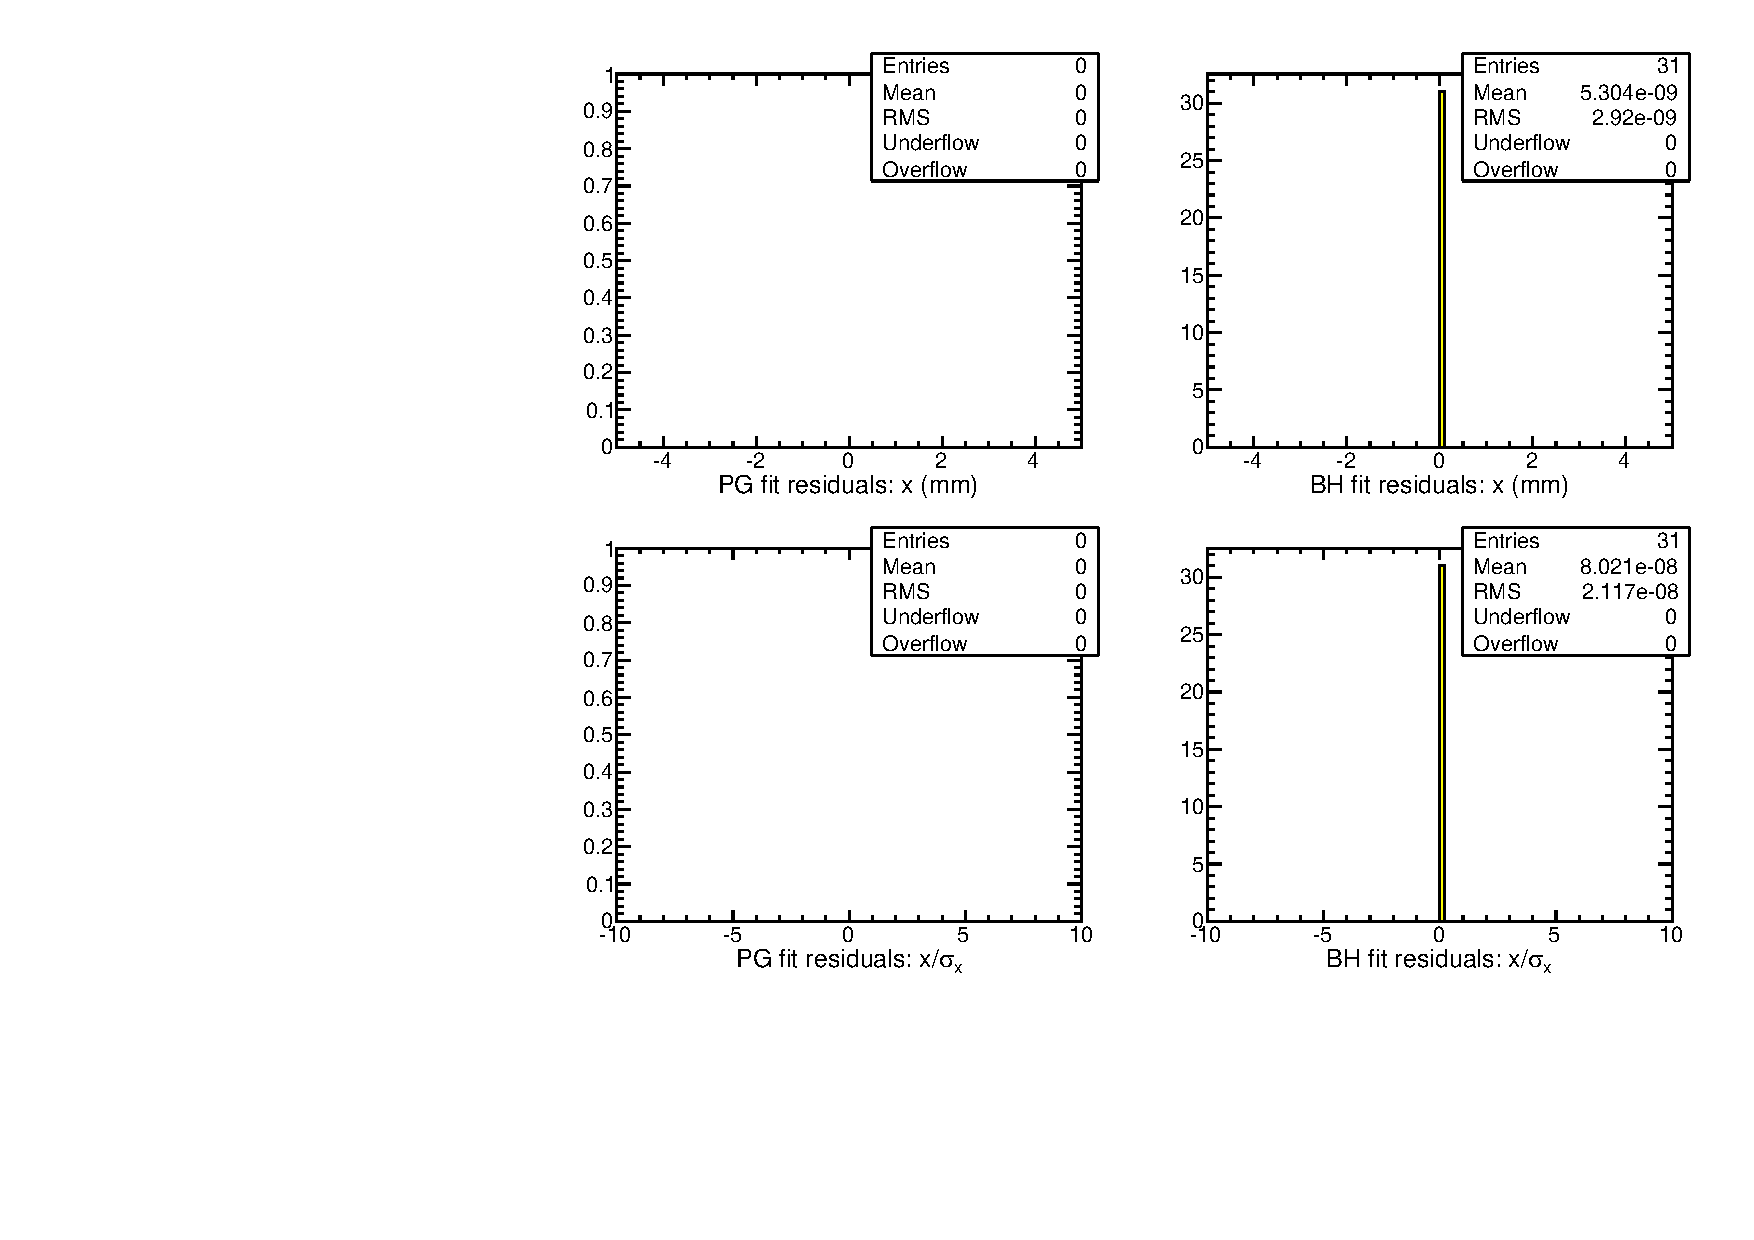
\includegraphics[width=0.9\linewidth]{newplots_fitresiduals_MEm1_1_x.pdf}}
\only<3>{Numbers in boxes are $\phi$ position uncertainty in each mode in rad

First 6 are completely undetermined (uncertainty is meaningless)

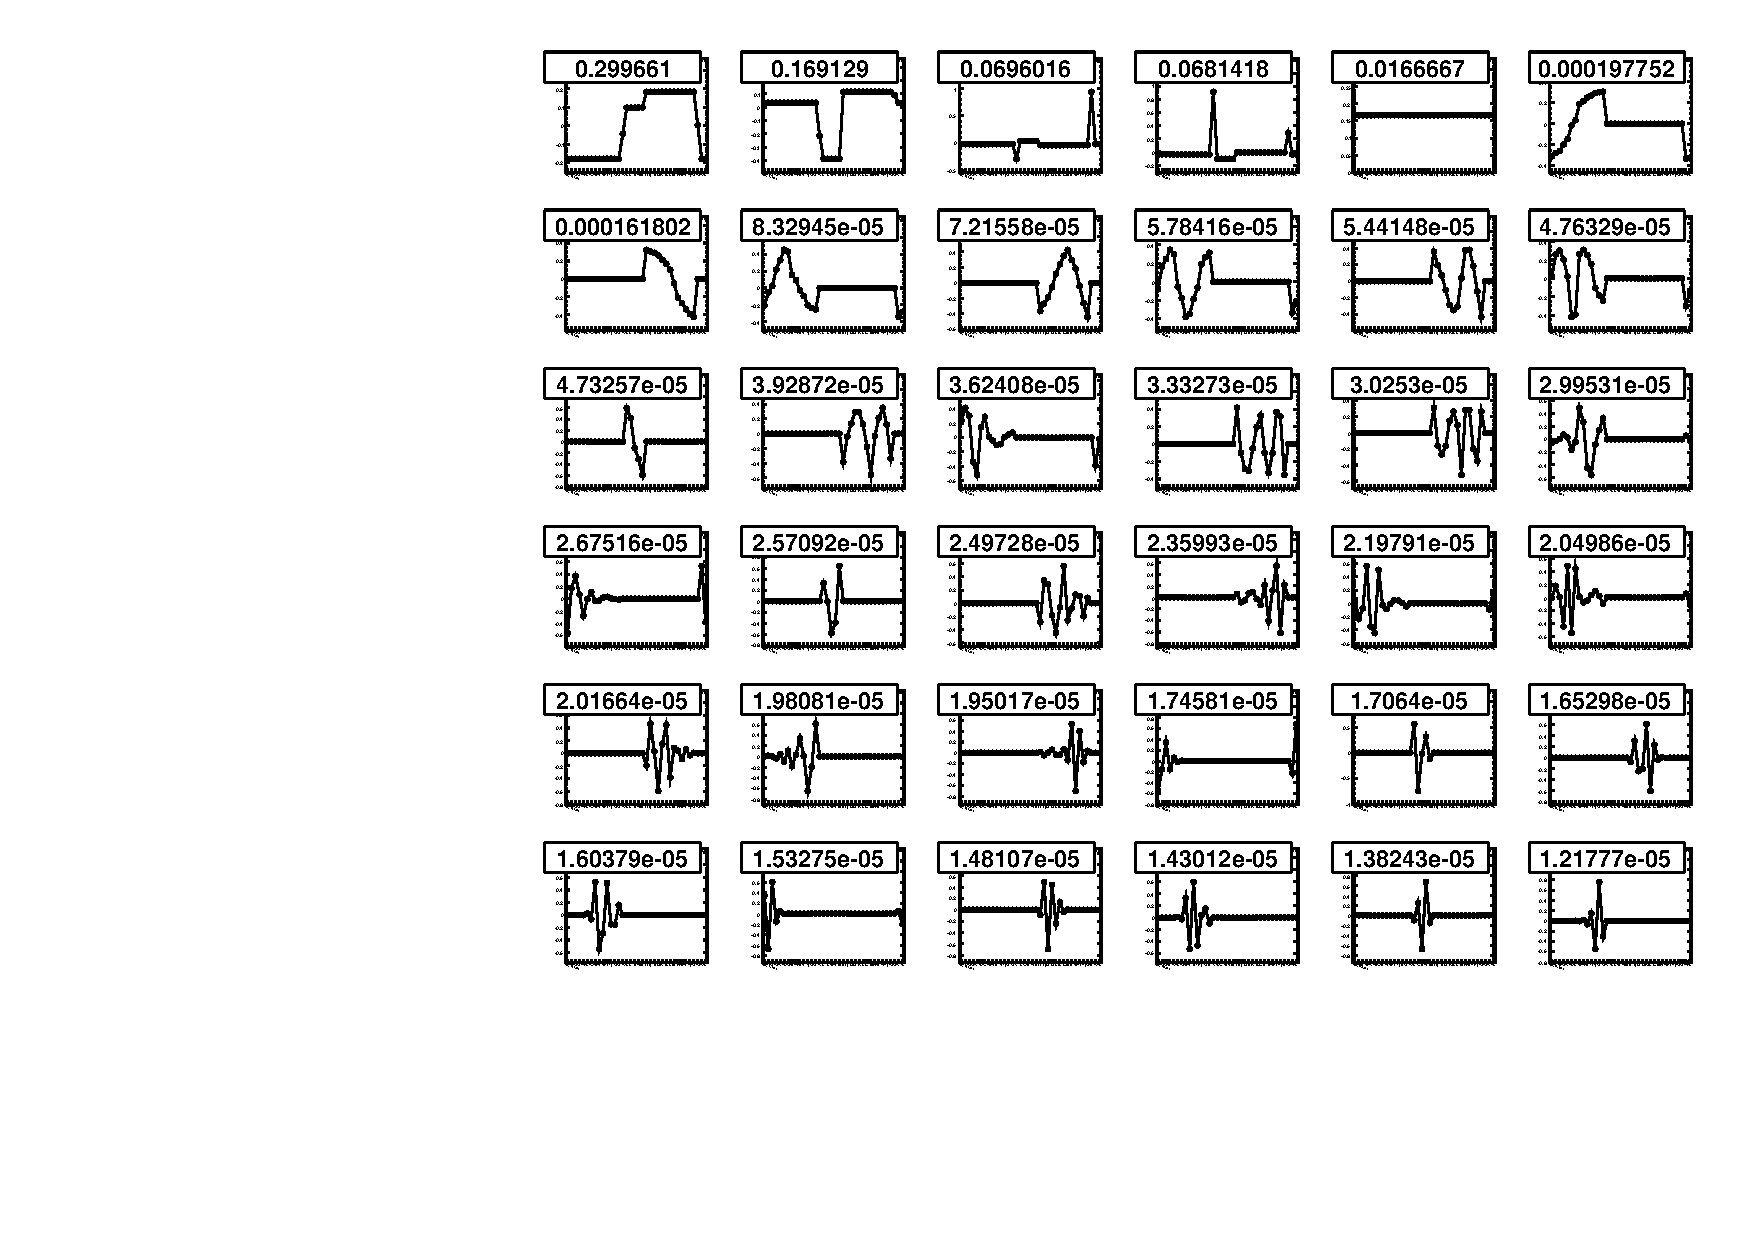
\includegraphics[width=0.9\linewidth]{newplots_errors_MEm1_1_x.pdf}}
\end{frame}

\begin{frame}
\frametitle{ME$-$1/1 $\phi_z$}

\only<1>{Convergence in $\phi_z$ angles

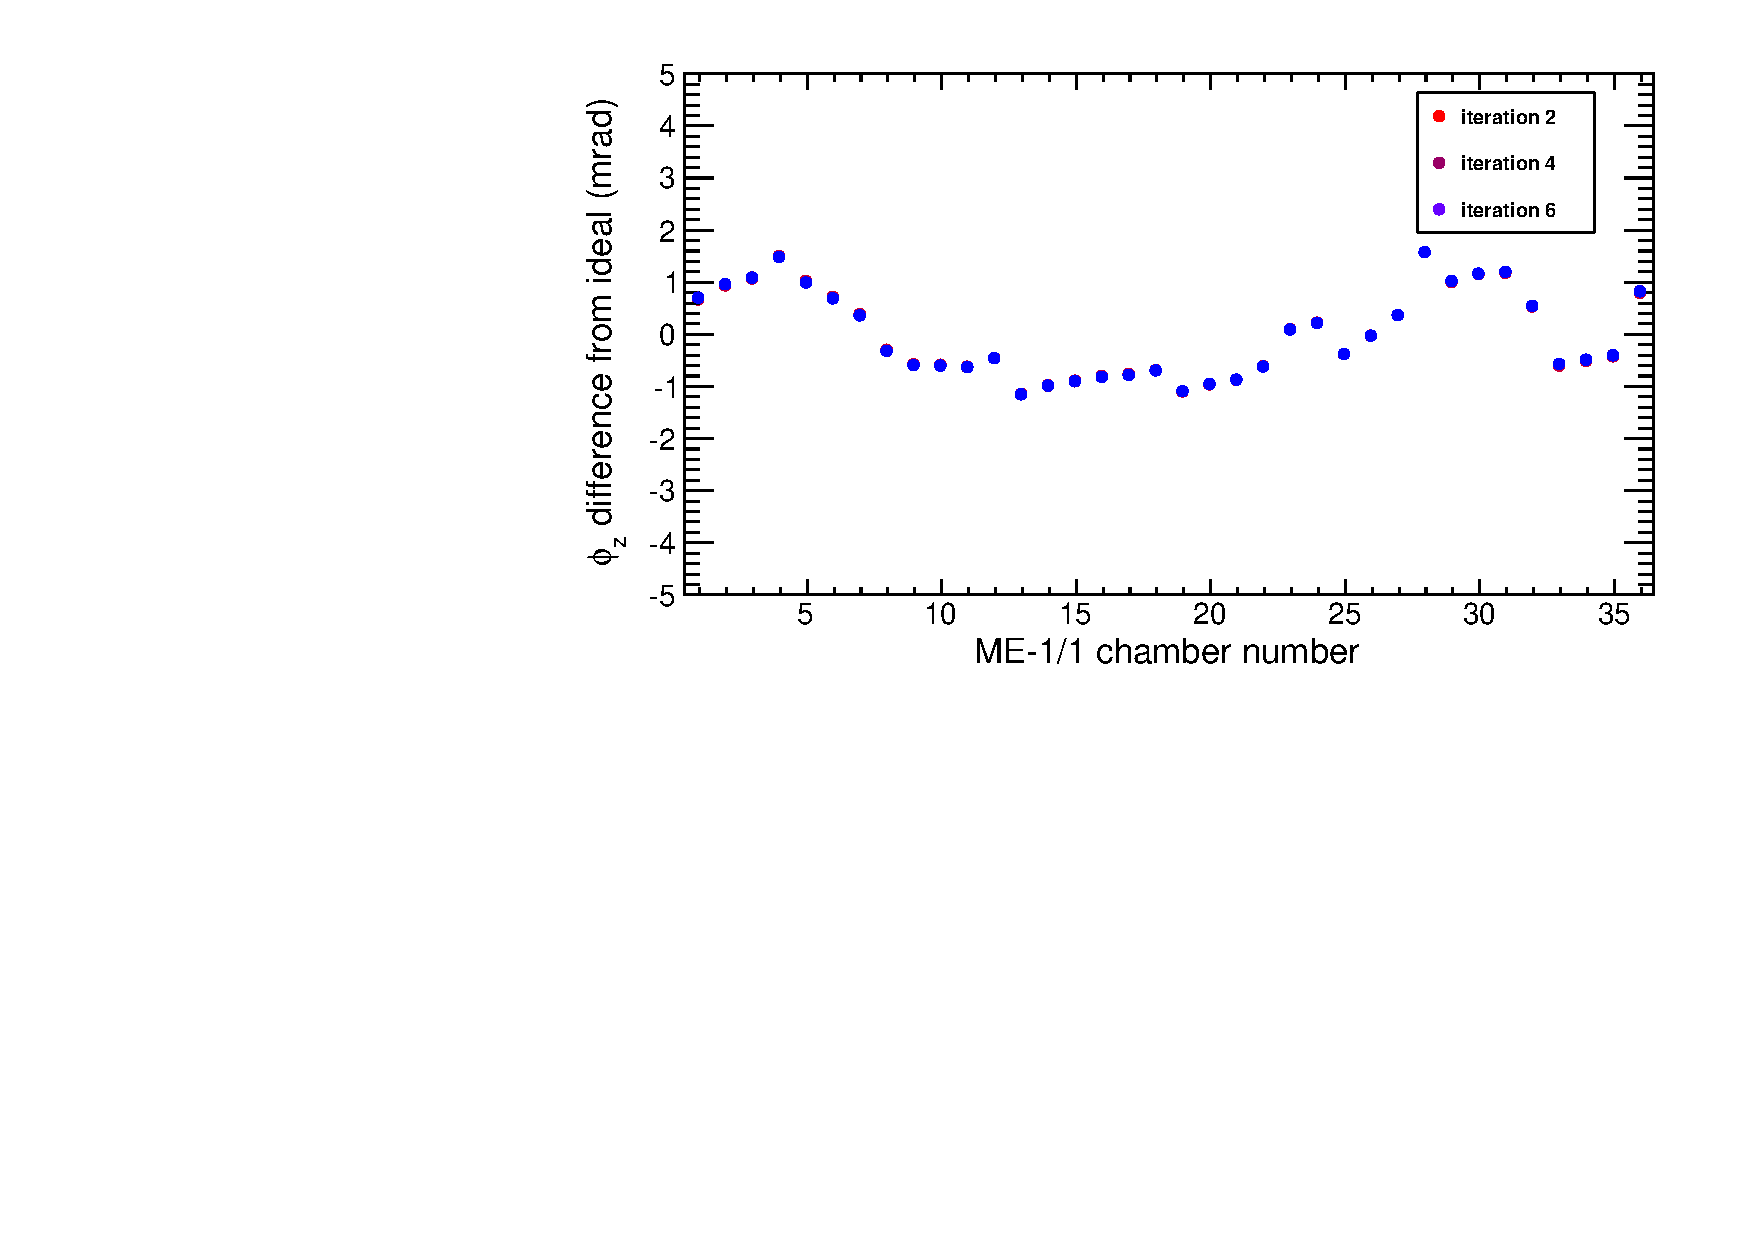
\includegraphics[width=\linewidth]{newplots_convergence_mem11_phiz.pdf}}
\only<2>{Fit residuals in $\phi_z$ (not track residuals): no PG, perfect BH fit

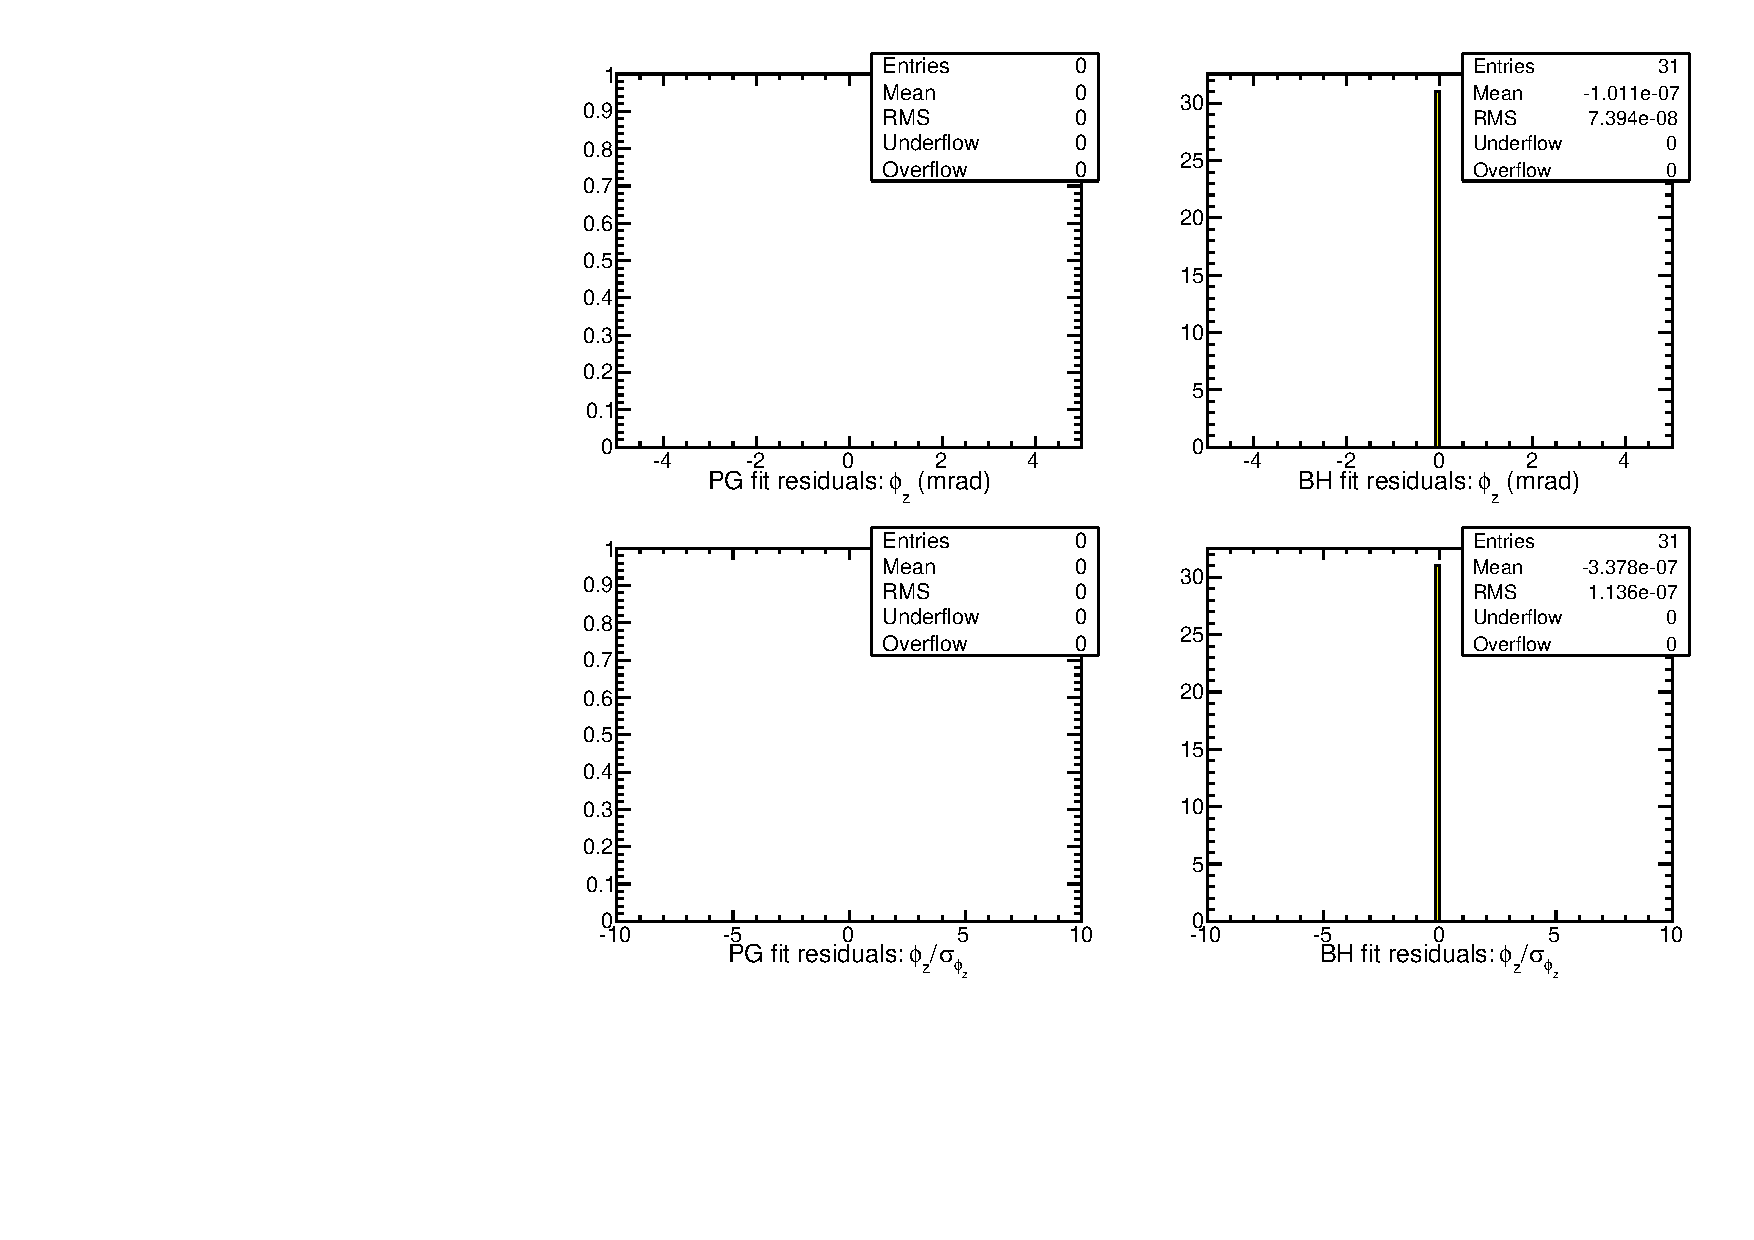
\includegraphics[width=0.9\linewidth]{newplots_fitresiduals_MEm1_1_phiz.pdf}}
\only<3>{Numbers in boxes are $\phi_z$ angle uncertainty in each mode in rad

First 7 are completely undetermined (uncertainty is meaningless)

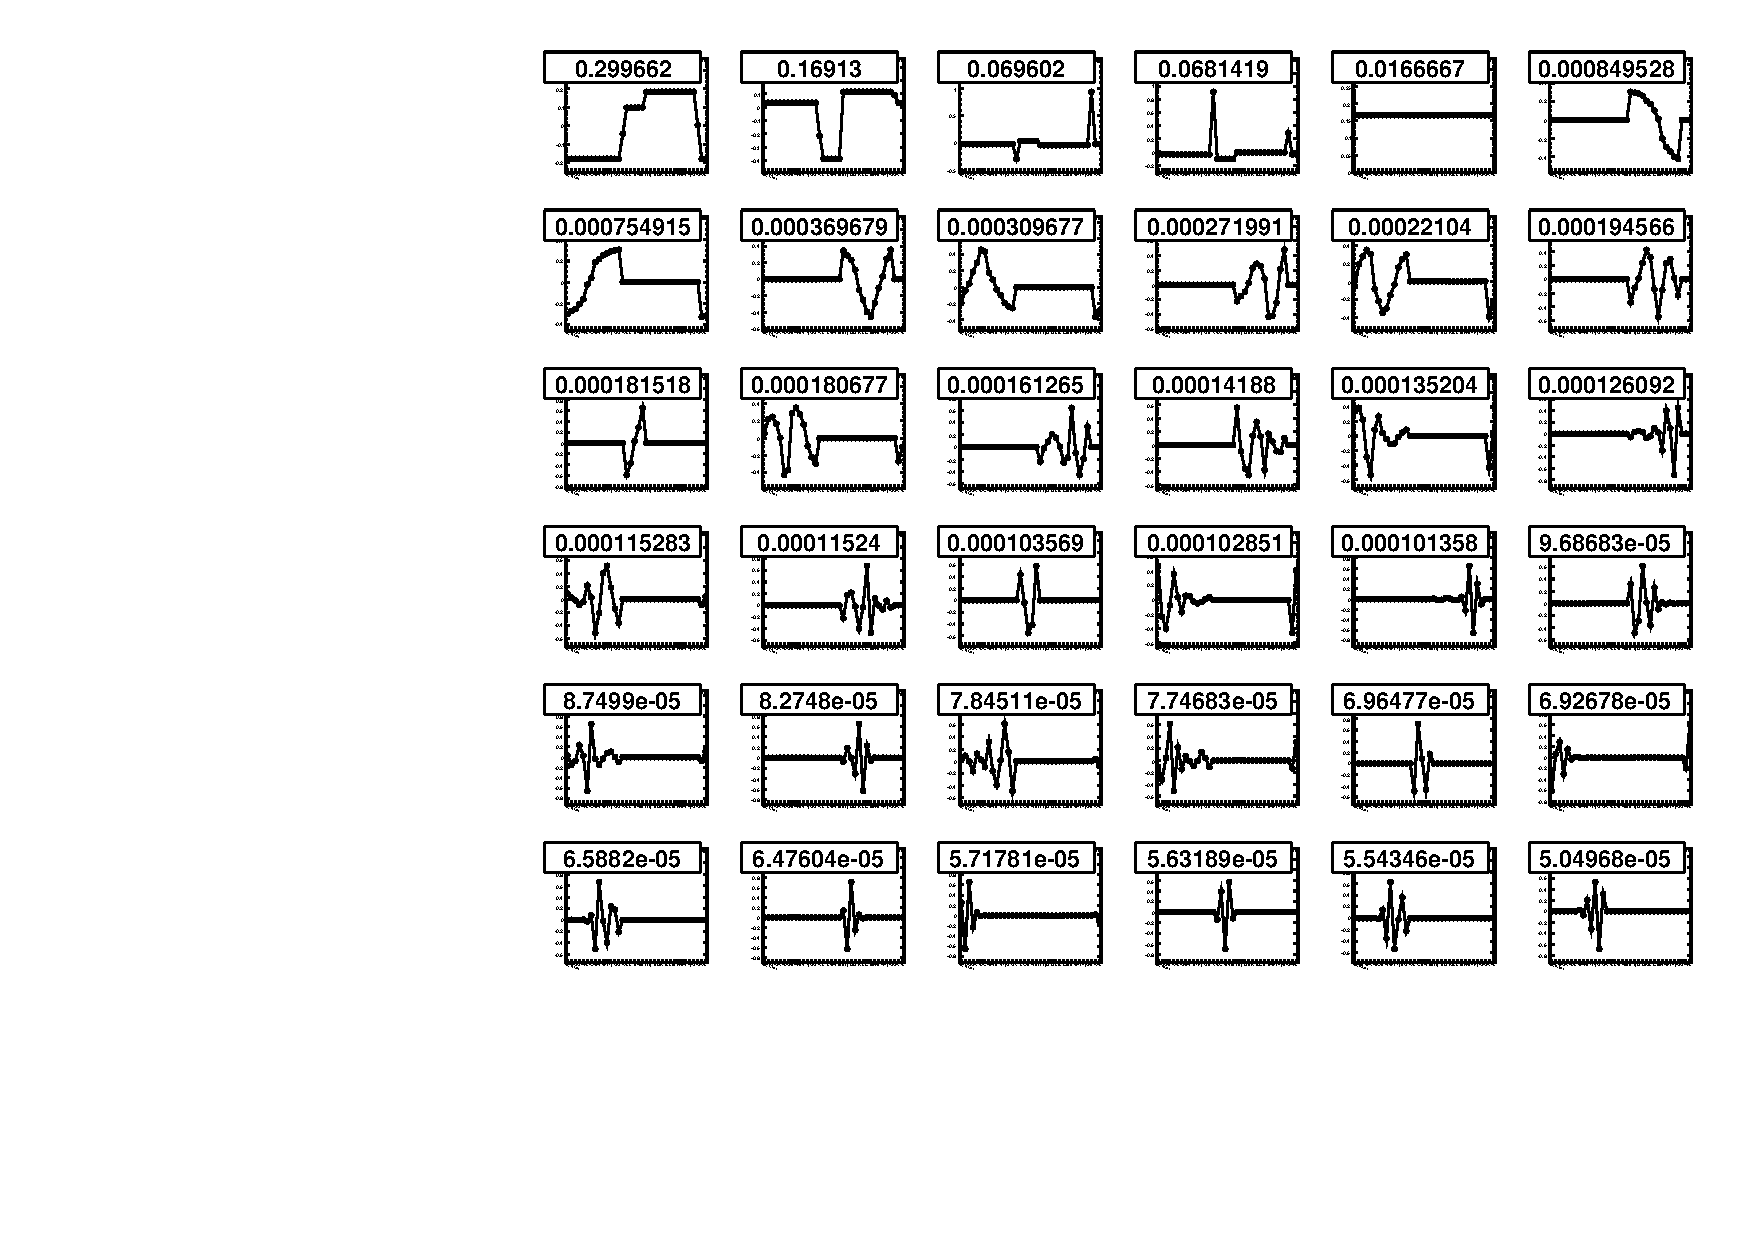
\includegraphics[width=0.9\linewidth]{newplots_errors_MEm1_1_phiz.pdf}}
\end{frame}

\begin{frame}
\frametitle{YE$+$1 $r\phi$}

\only<1>{Convergence in $r\phi$ positions

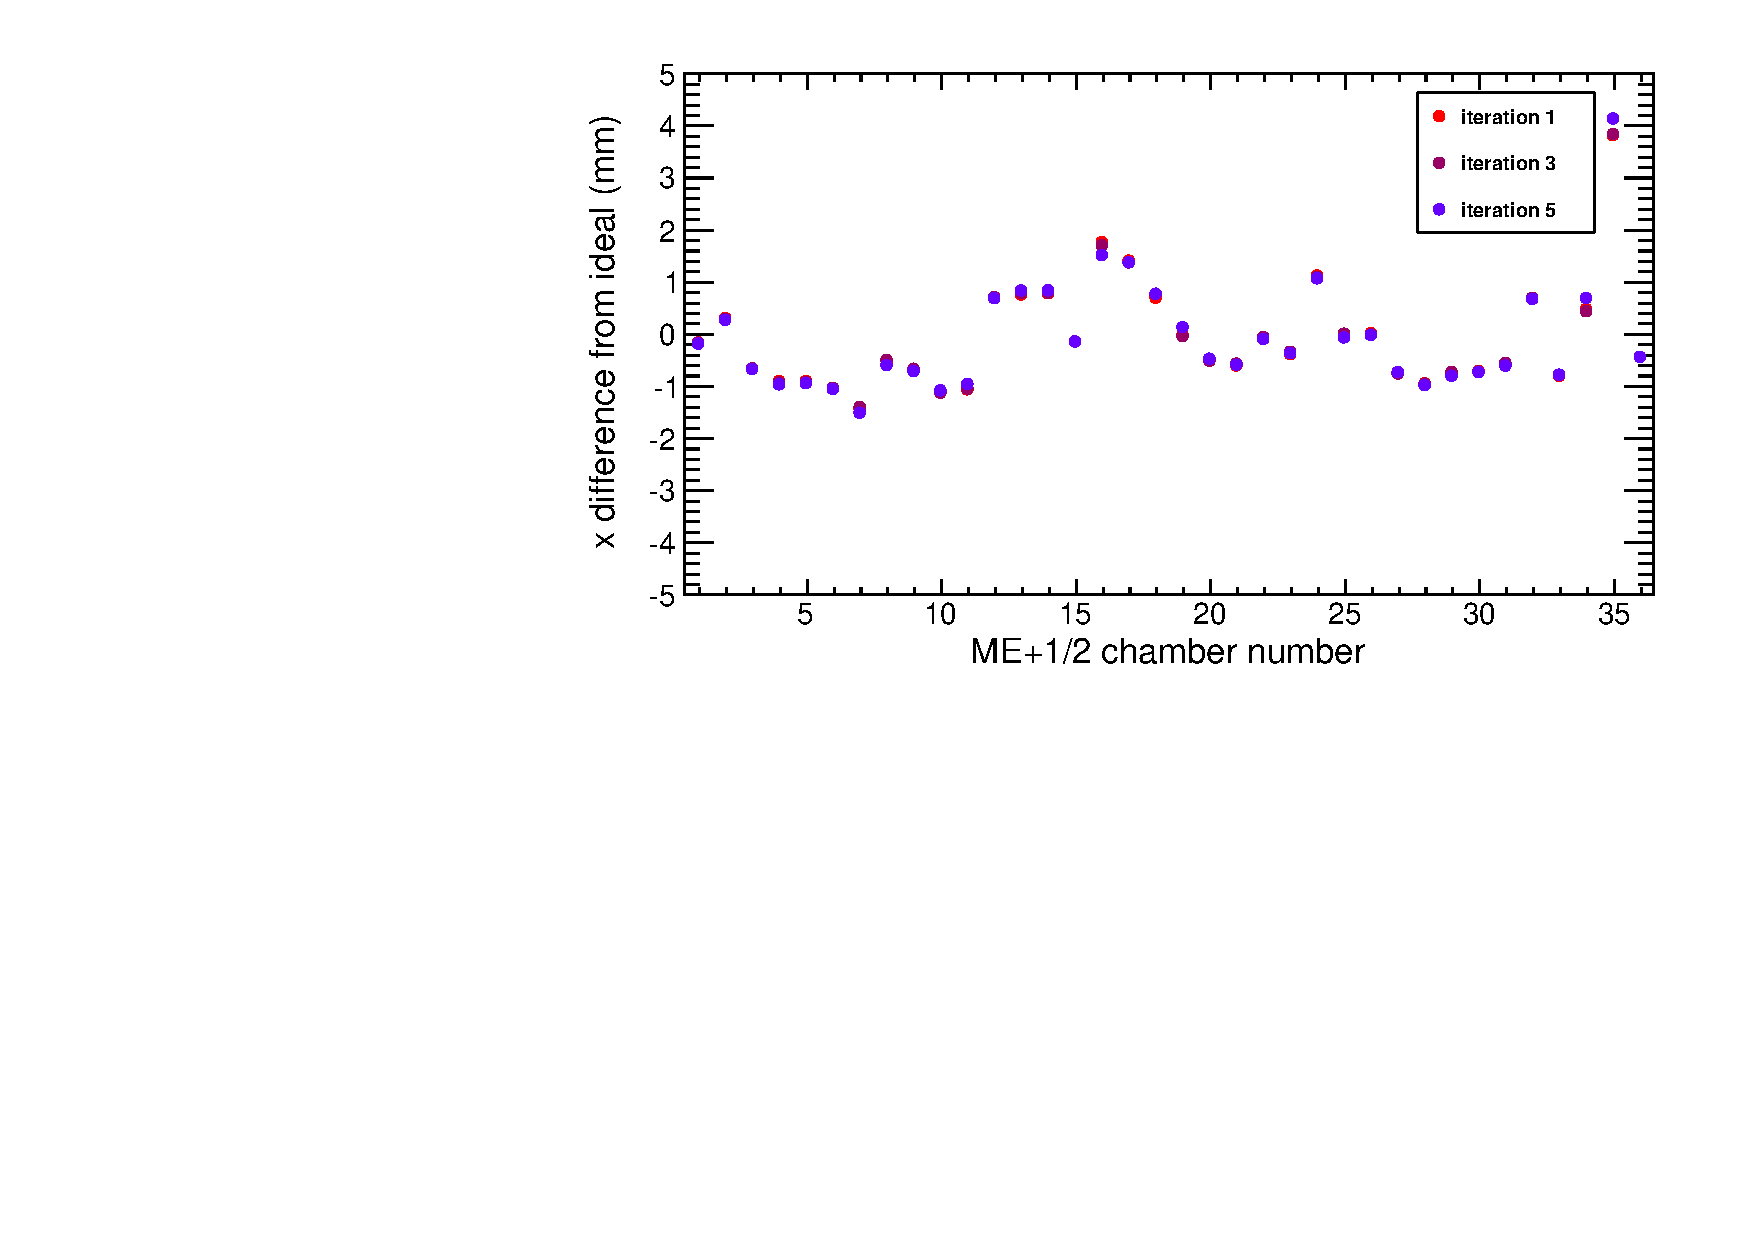
\includegraphics[width=0.6\linewidth]{newplots_convergence_mep12_x.pdf}

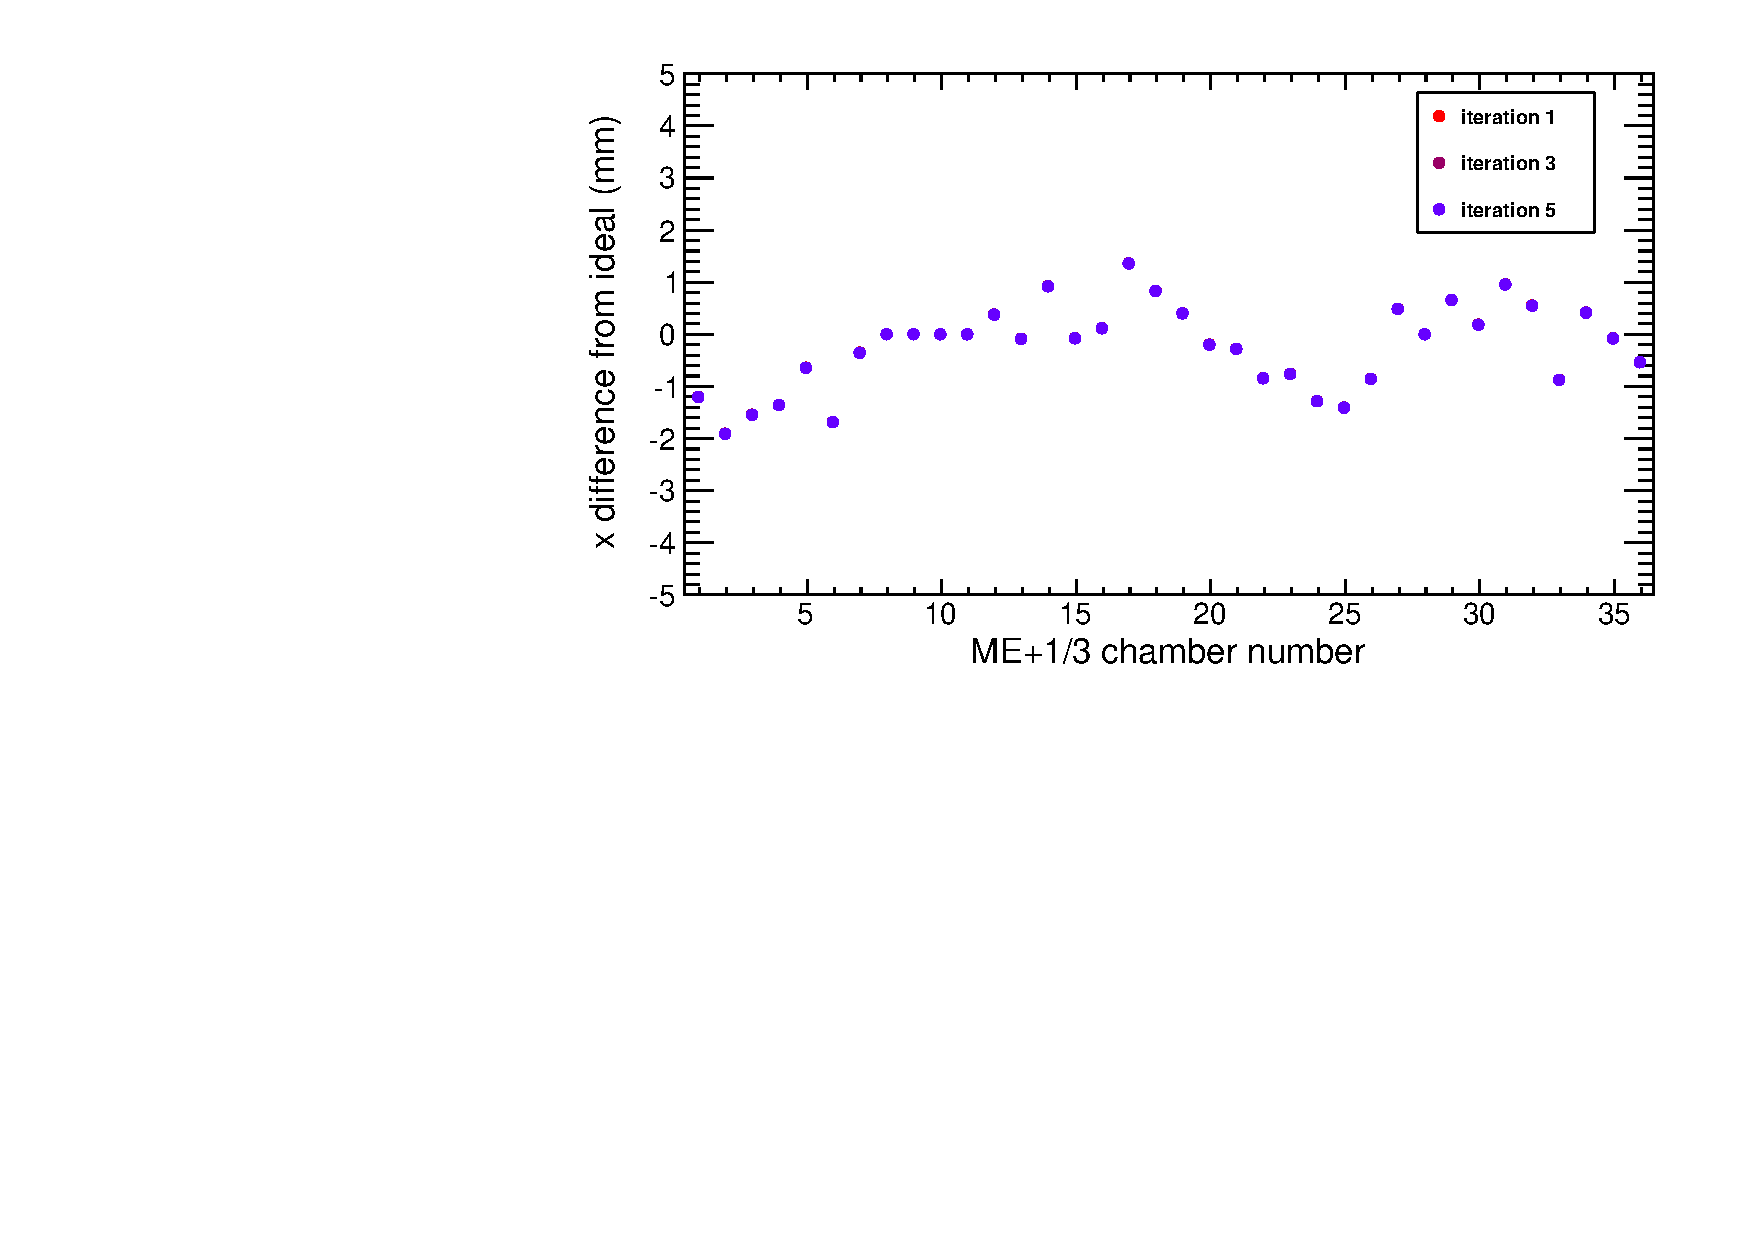
\includegraphics[width=0.6\linewidth]{newplots_convergence_mep13_x.pdf}}
\only<2>{Fit residuals in $r\phi$ (not track residuals): no BH in ME$+$1/3 (green)

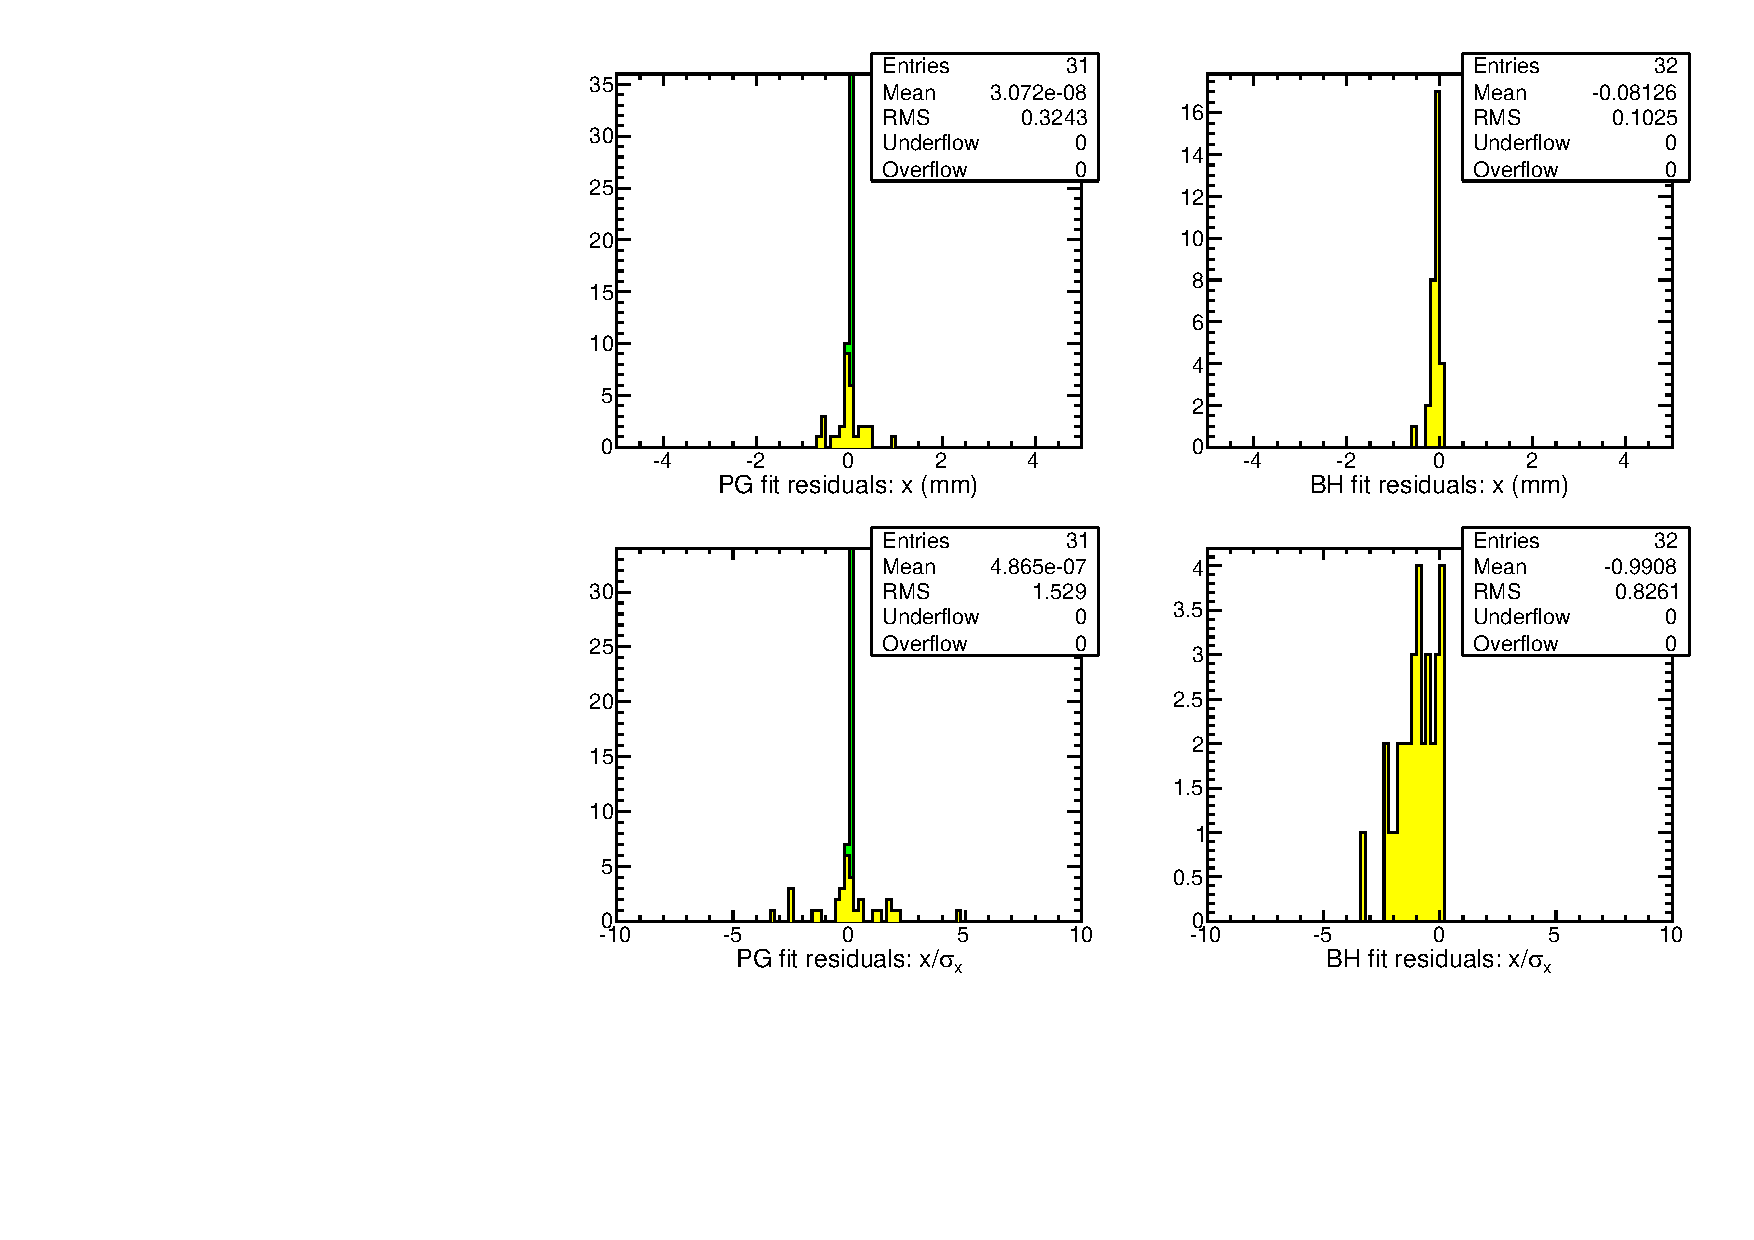
\includegraphics[width=0.9\linewidth]{newplots_fitresiduals_YEp1_x.pdf}}
\only<3>{Numbers in boxes are $\phi$ position uncertainty in each mode in rad

First 1 is completely undetermined (uncertainty is meaningless)

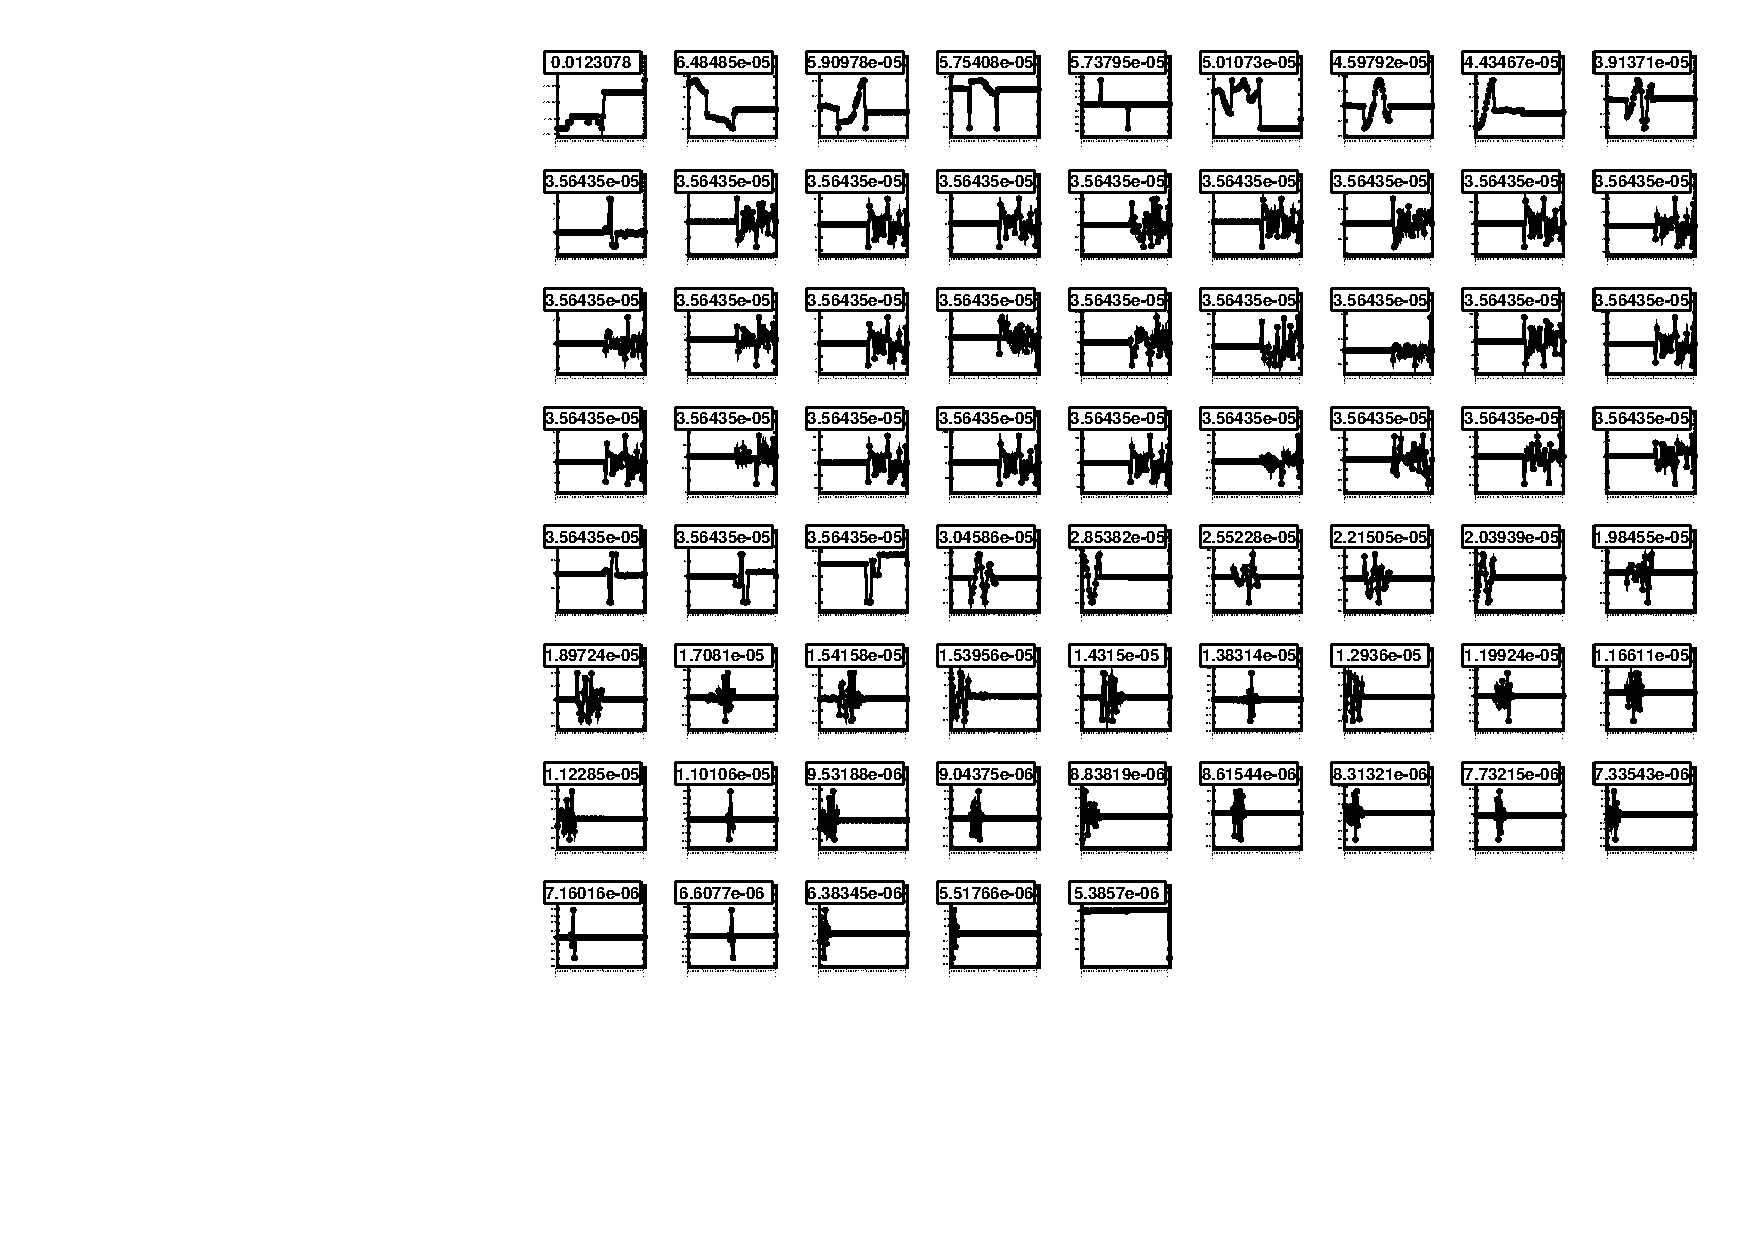
\includegraphics[width=0.9\linewidth]{newplots_errors_YEp1_x.pdf}}
\end{frame}

\begin{frame}
\frametitle{YE$+$1 $\phi_z$}

\only<1>{Convergence in $\phi_z$ positions

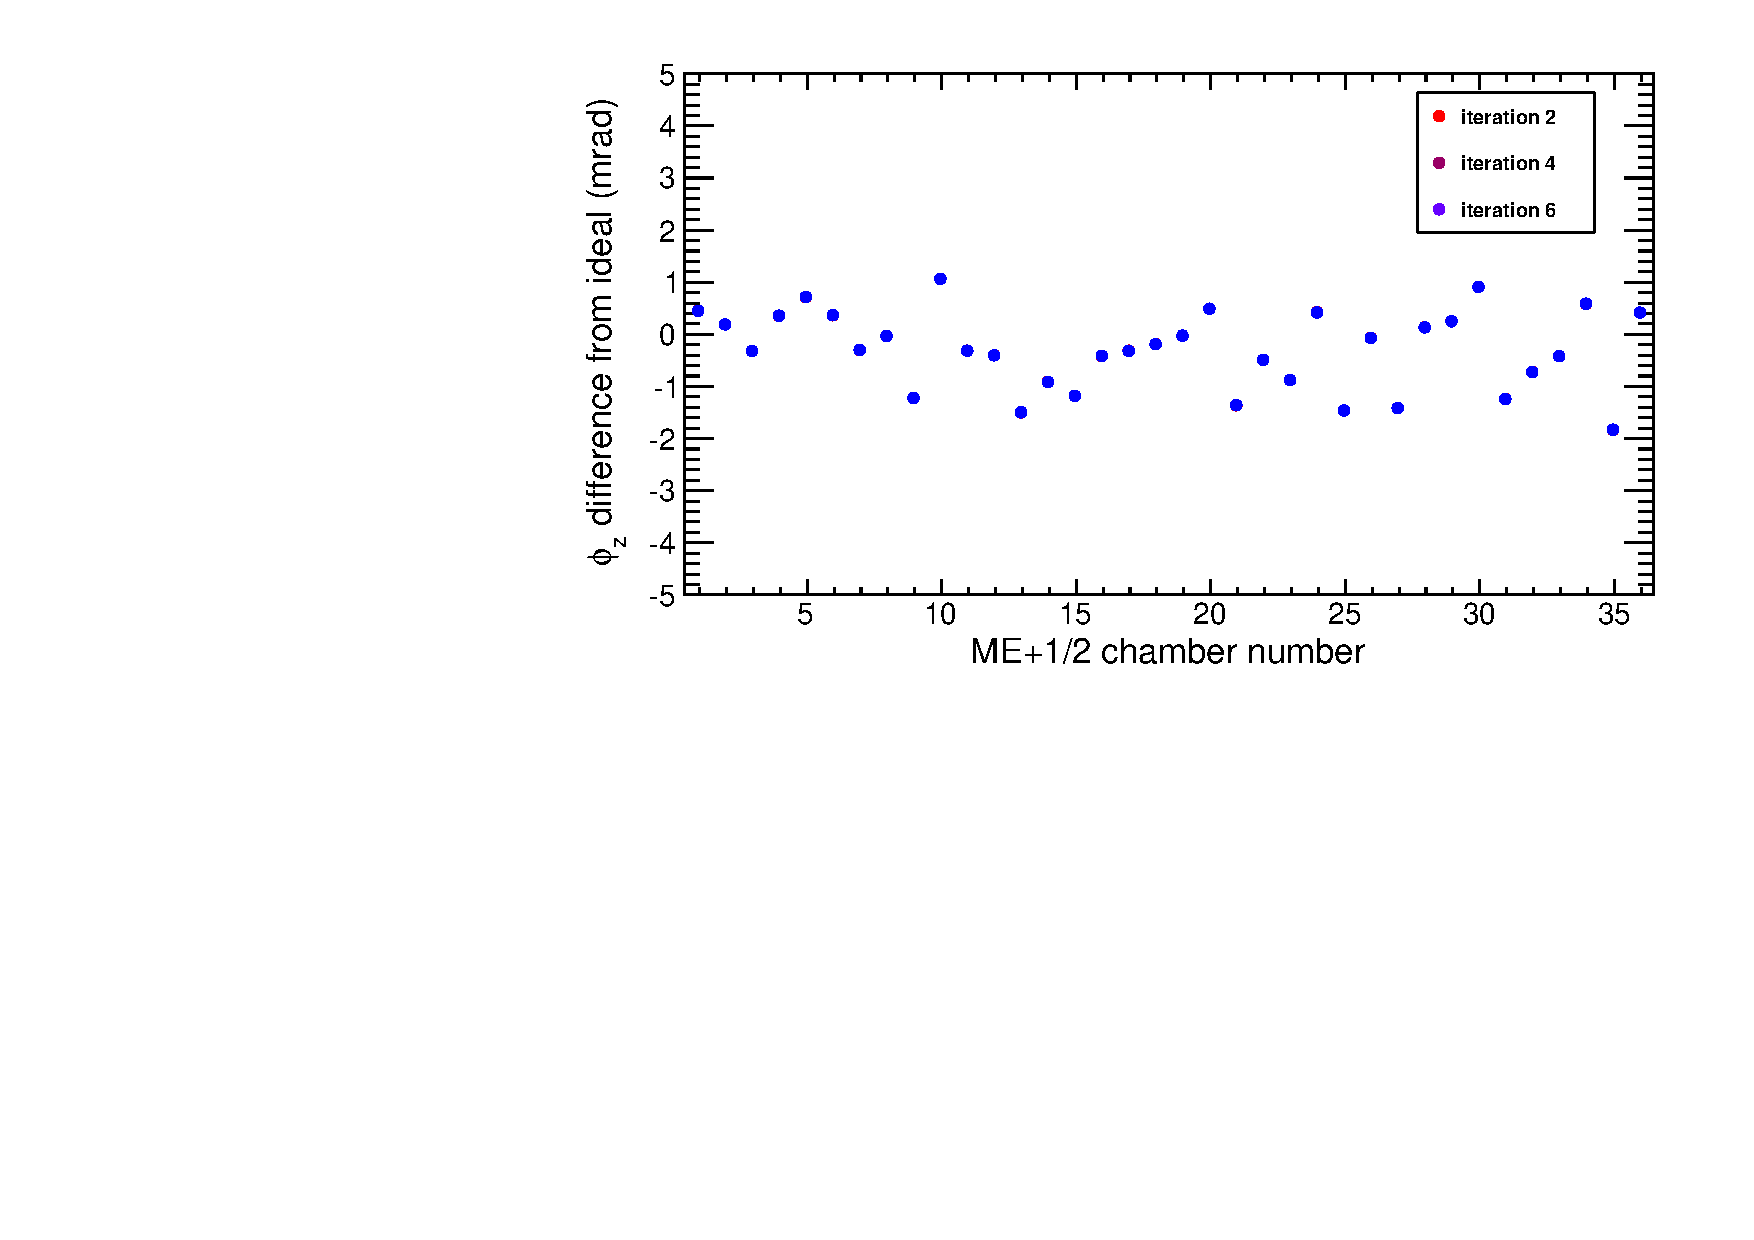
\includegraphics[width=0.6\linewidth]{newplots_convergence_mep12_phiz.pdf}

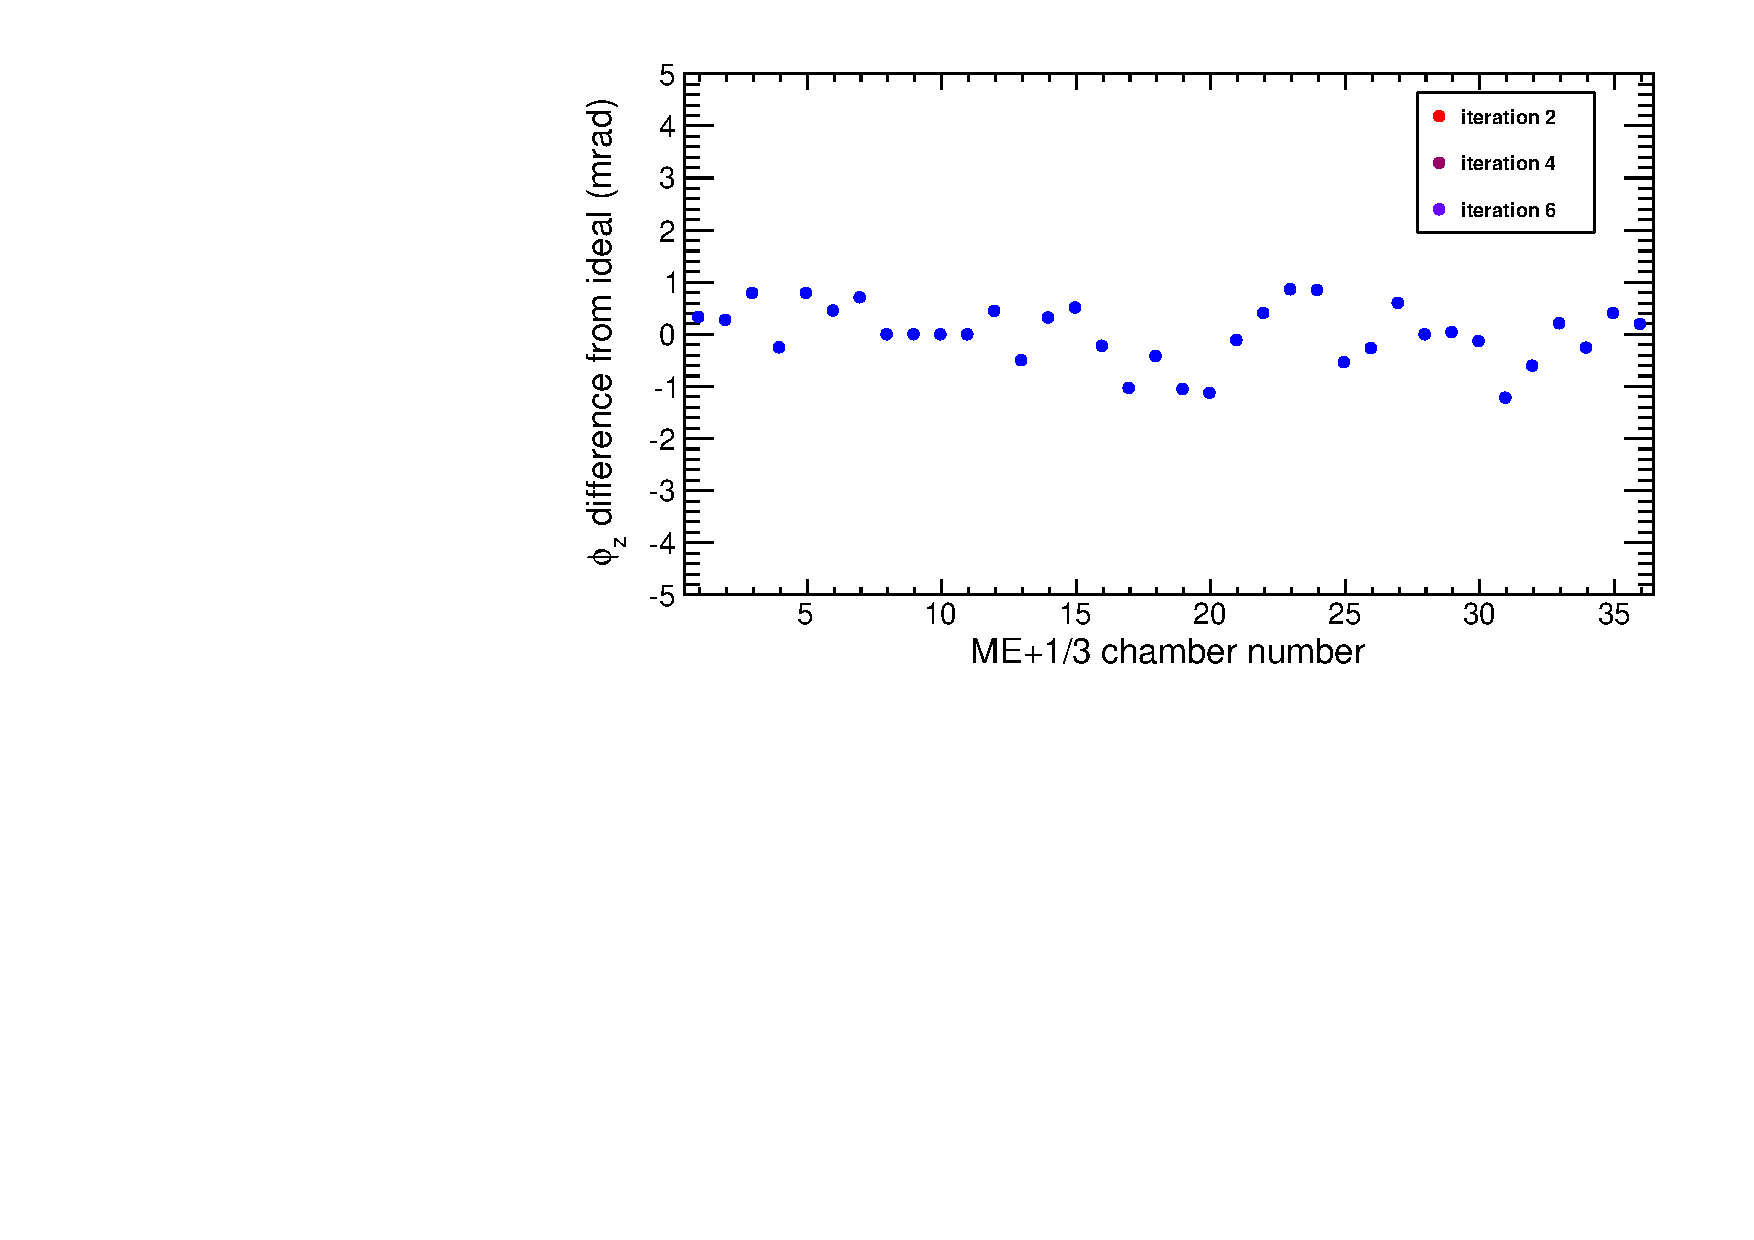
\includegraphics[width=0.6\linewidth]{newplots_convergence_mep13_phiz.pdf}}
\only<2>{Fit residuals in $\phi_z$ (not track residuals): no BH in ME$+$1/3 (green)

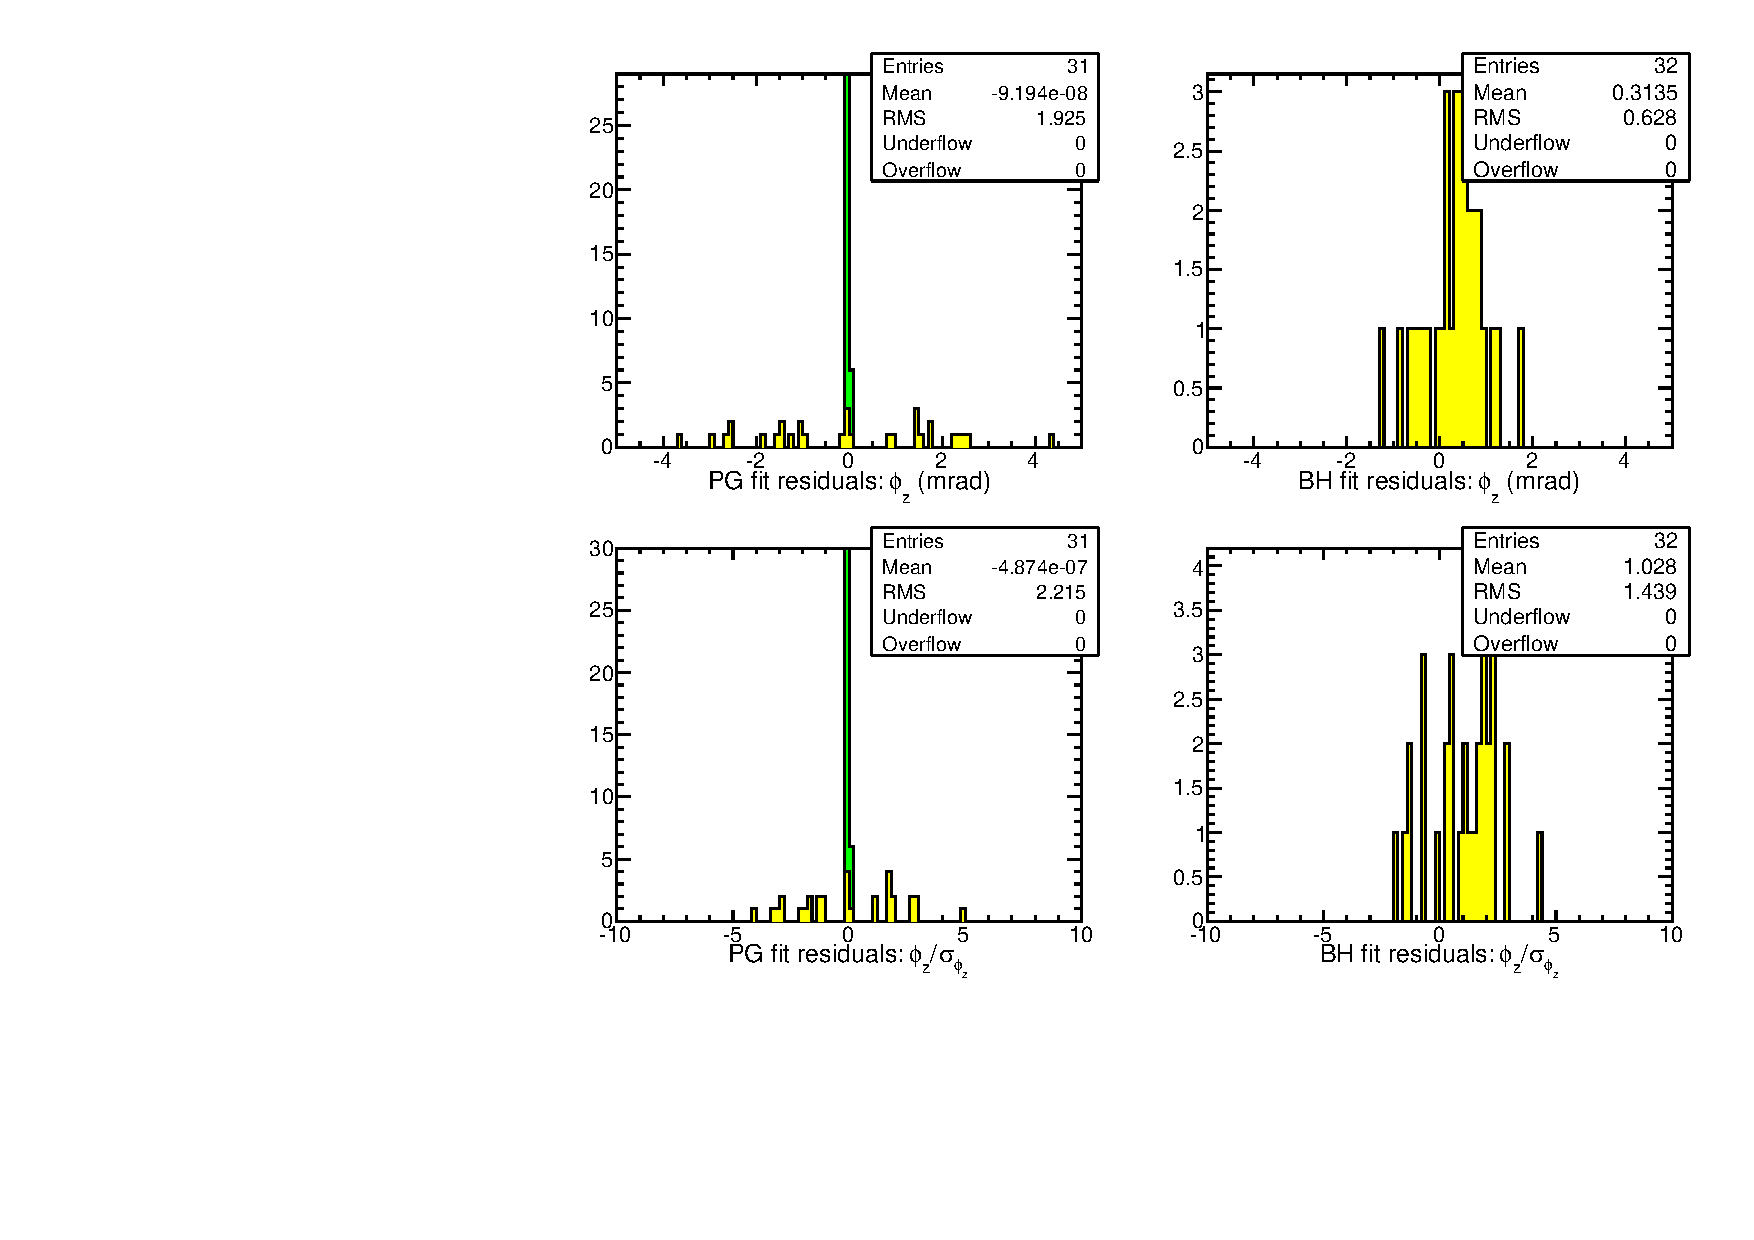
\includegraphics[width=0.9\linewidth]{newplots_fitresiduals_YEp1_phiz.pdf}}
\only<3>{Numbers in boxes are $\phi_z$ angle uncertainty in each mode in rad

First 1 is completely undetermined (uncertainty is meaningless)

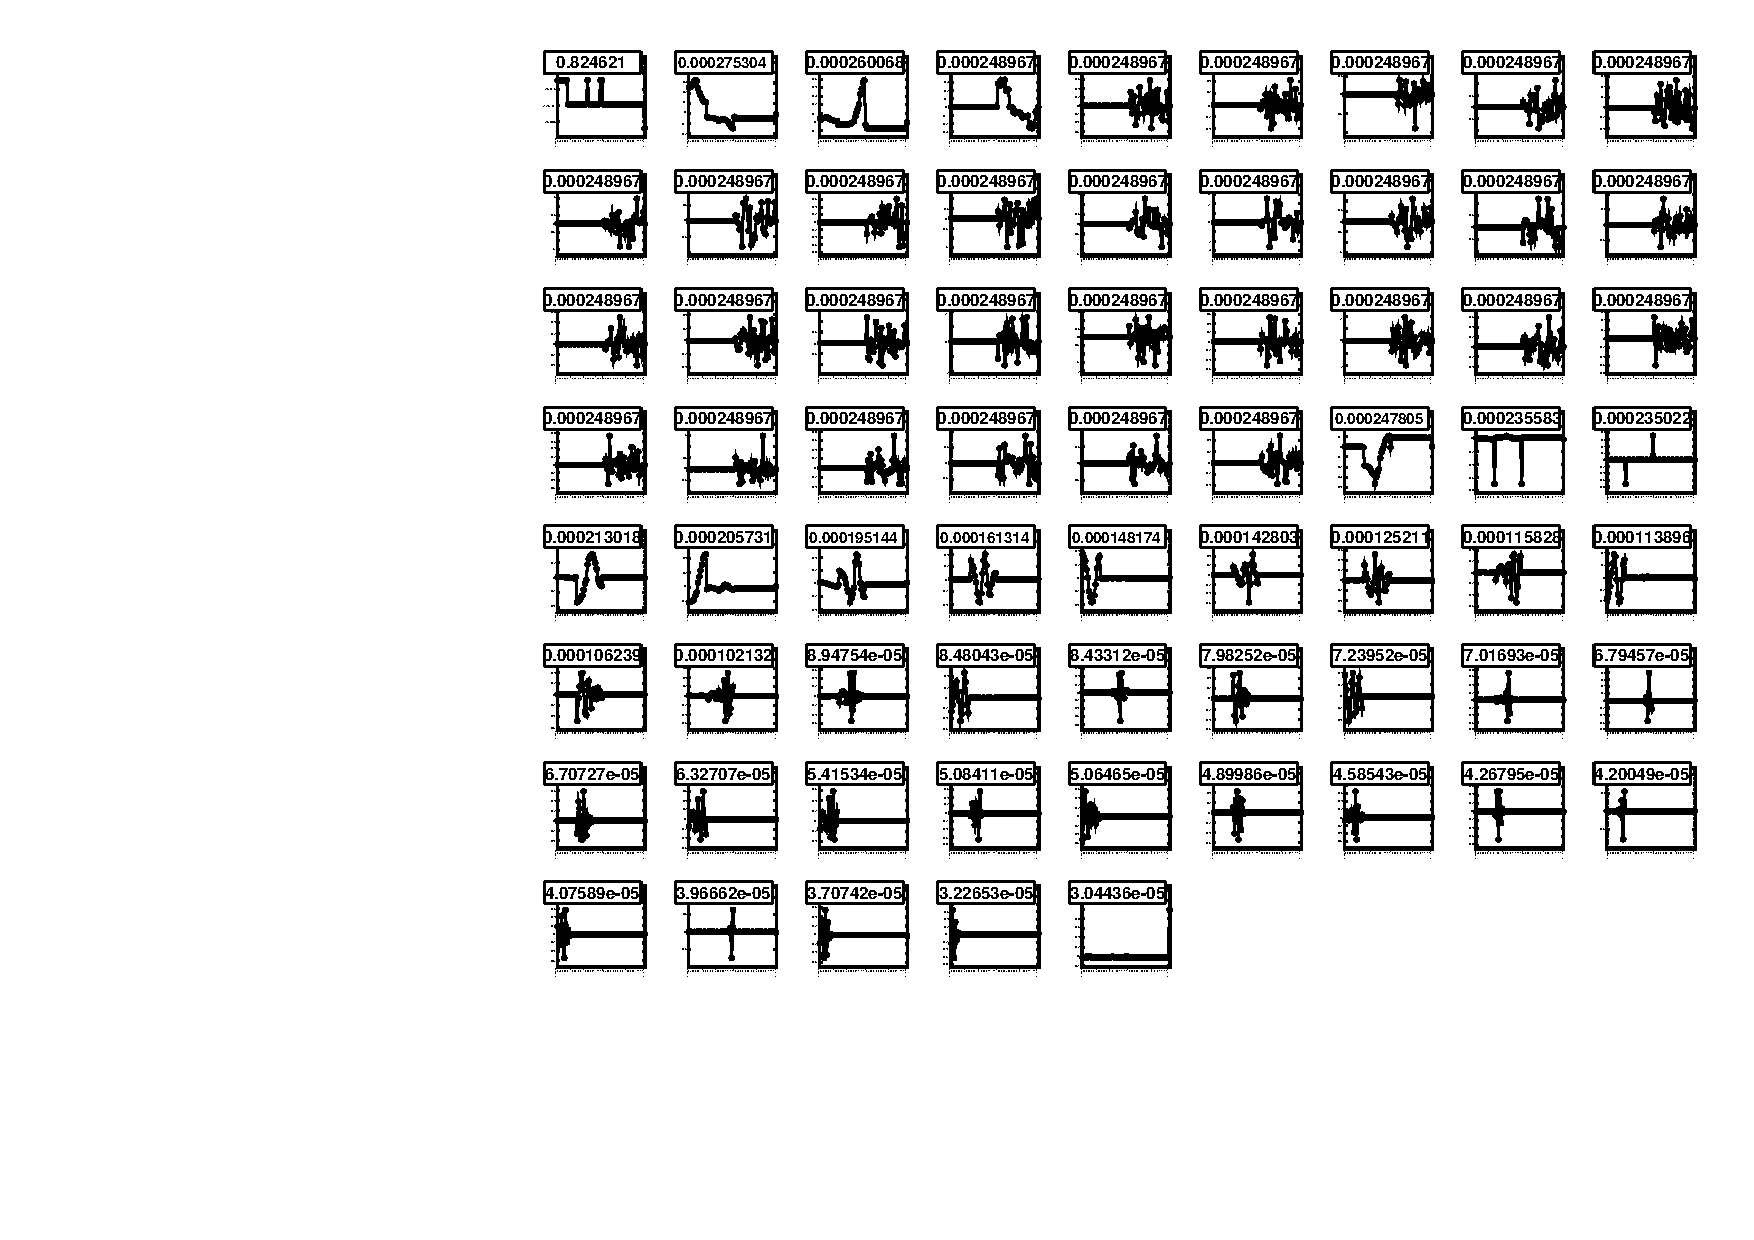
\includegraphics[width=0.9\linewidth]{newplots_errors_YEp1_phiz.pdf}}
\end{frame}

\begin{frame}
\frametitle{YE$-$1 $r\phi$}

\only<1>{Convergence in $r\phi$ positions

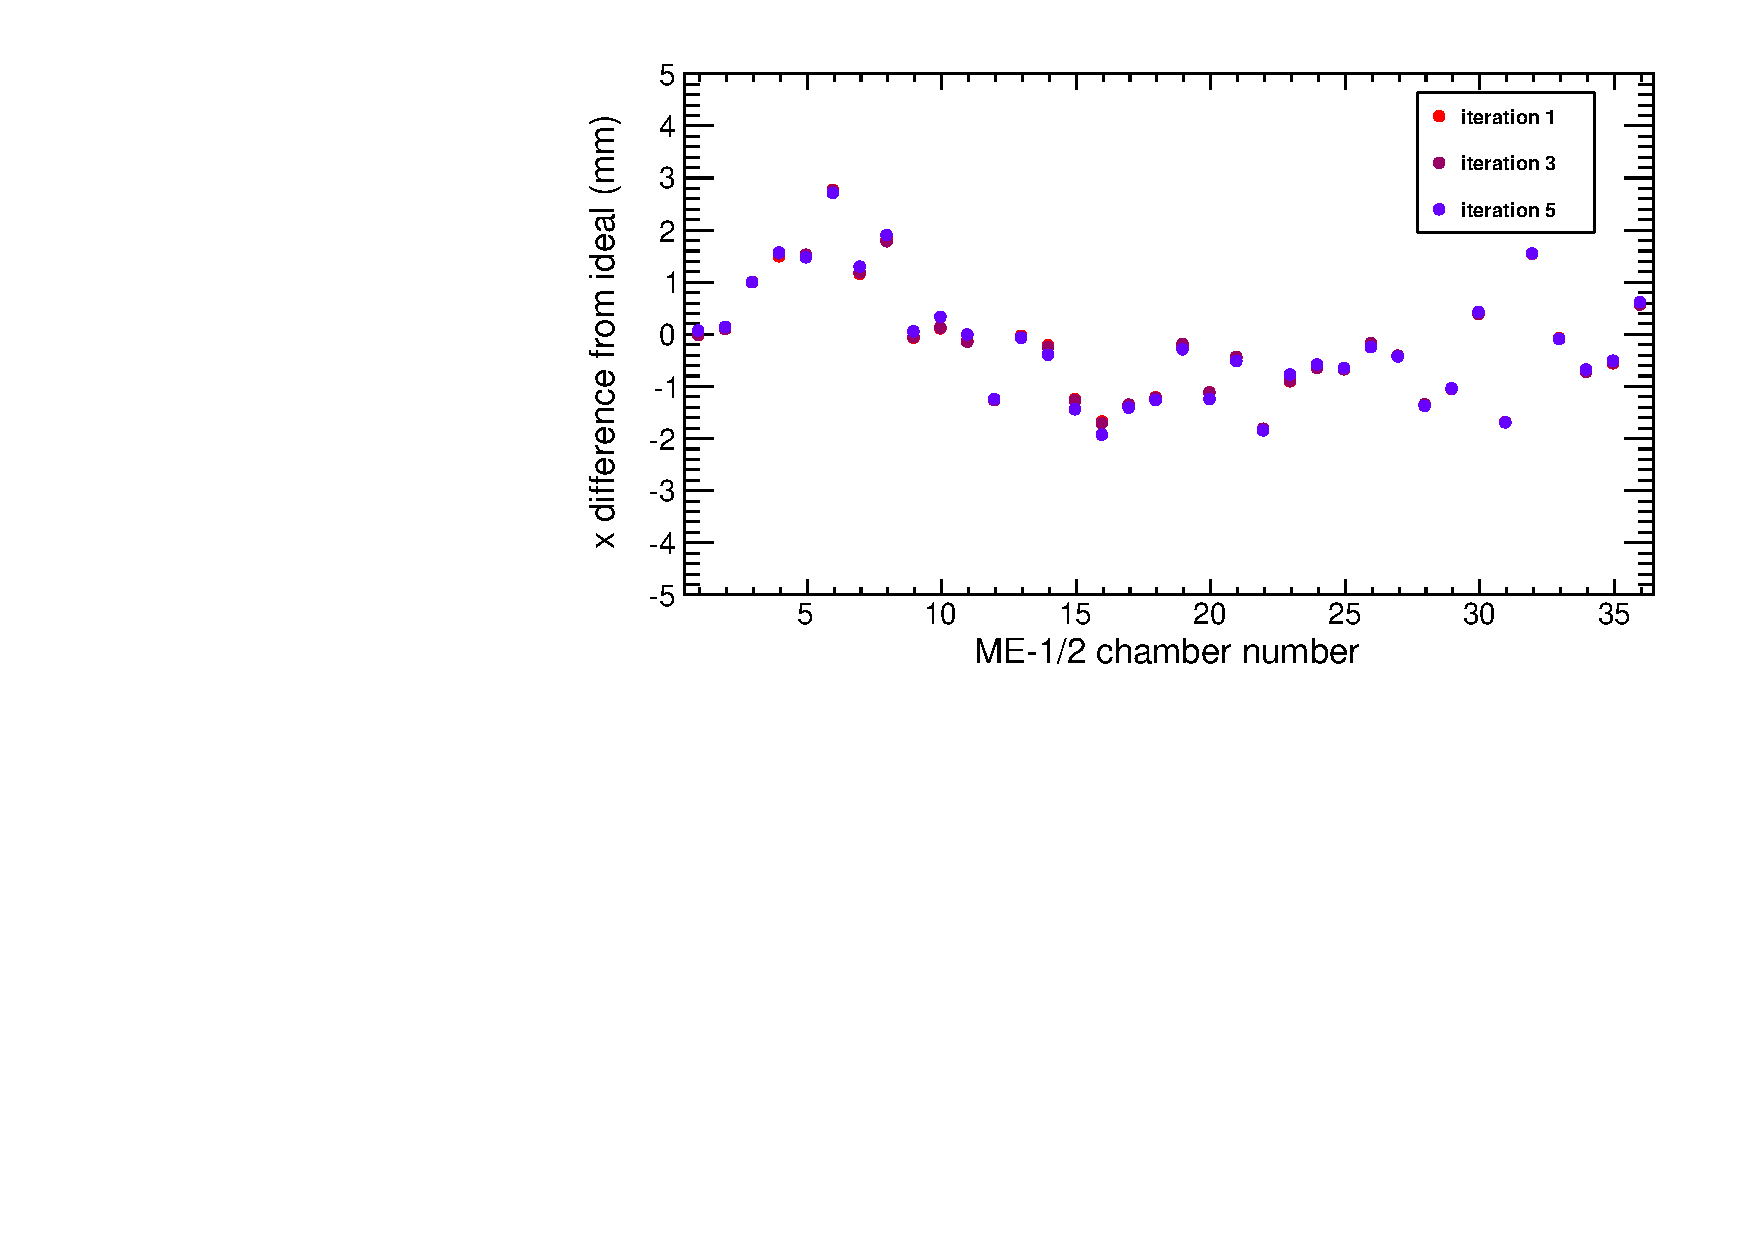
\includegraphics[width=0.6\linewidth]{newplots_convergence_mem12_x.pdf}

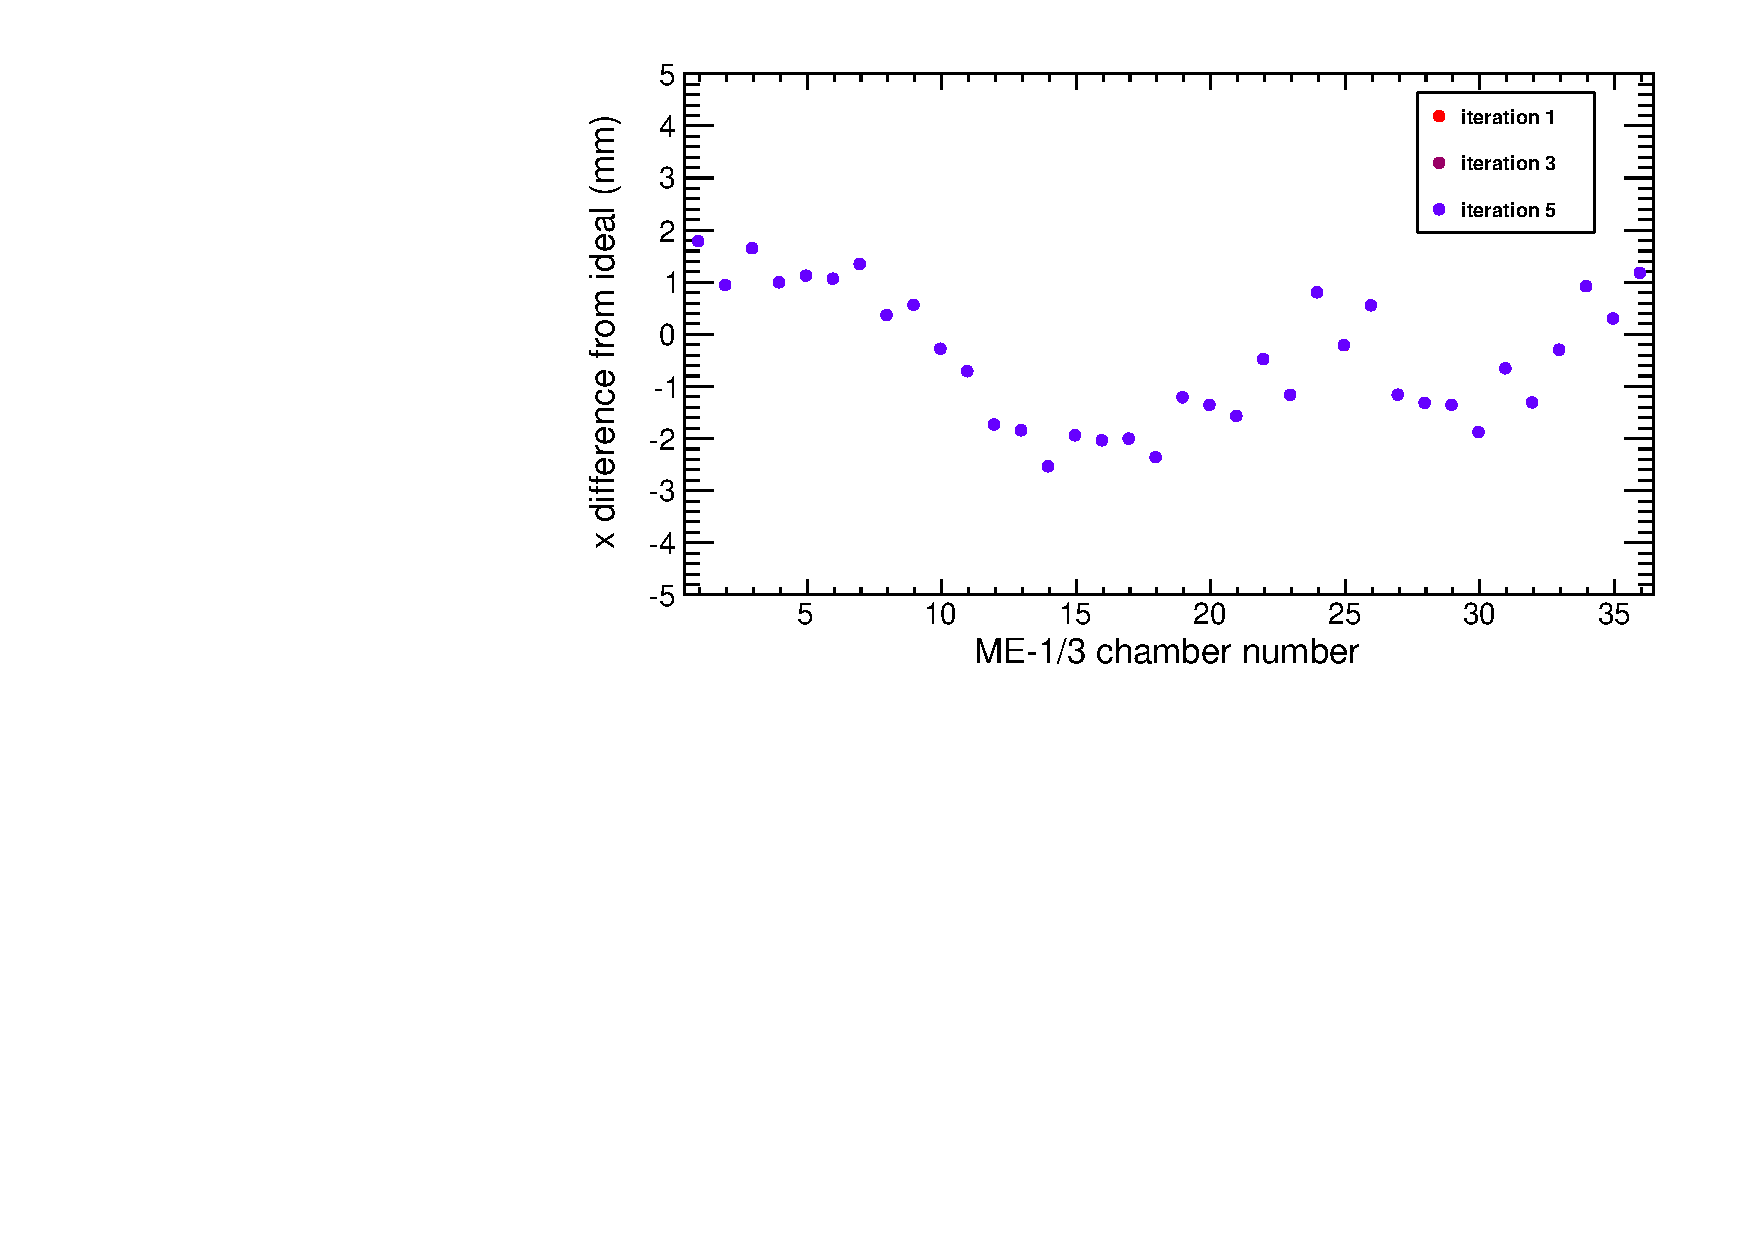
\includegraphics[width=0.6\linewidth]{newplots_convergence_mem13_x.pdf}}
\only<2>{Fit residuals in $r\phi$ (not track residuals): no BH in ME$-$1/3 (green)

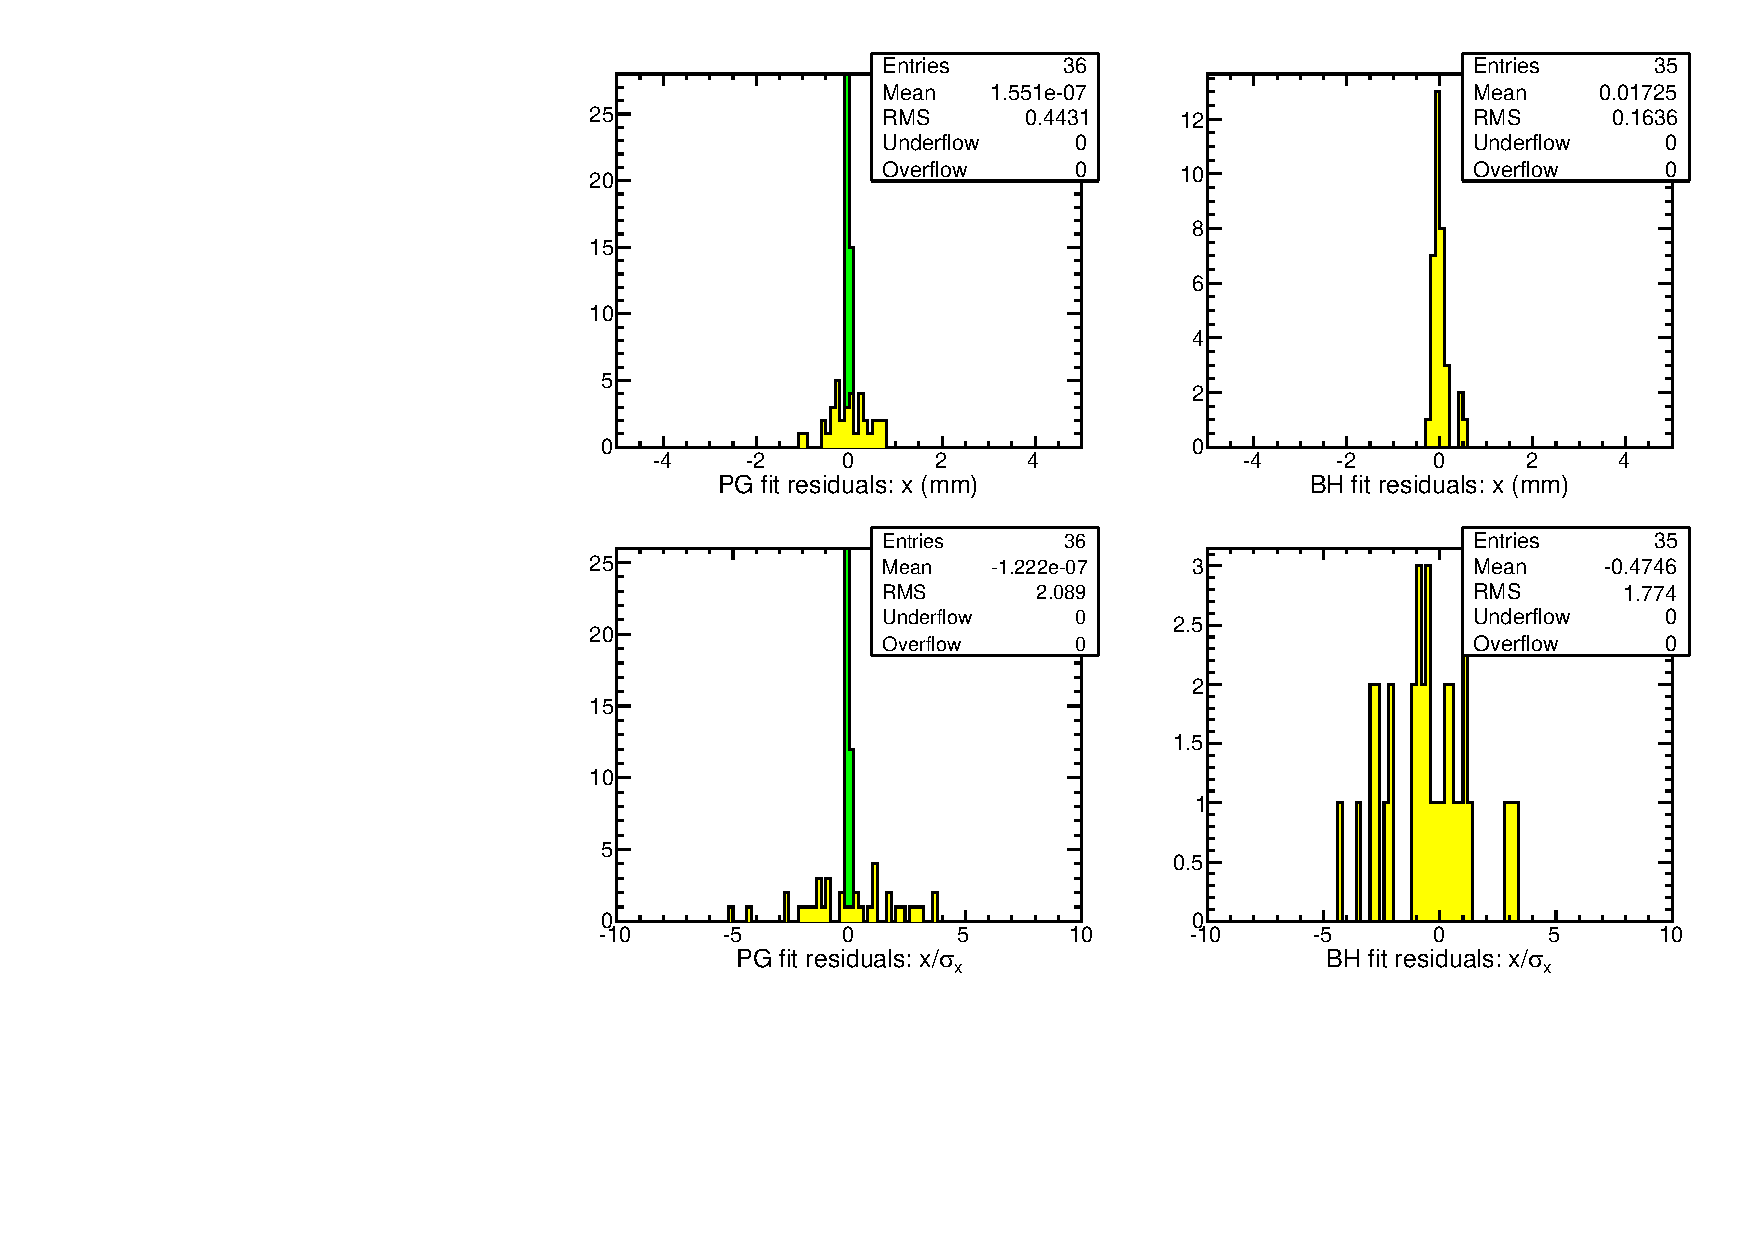
\includegraphics[width=0.9\linewidth]{newplots_fitresiduals_YEm1_x.pdf}}
\only<3>{Numbers in boxes are $\phi$ position uncertainty in each mode in rad

First 1 is completely undetermined (uncertainty is meaningless)

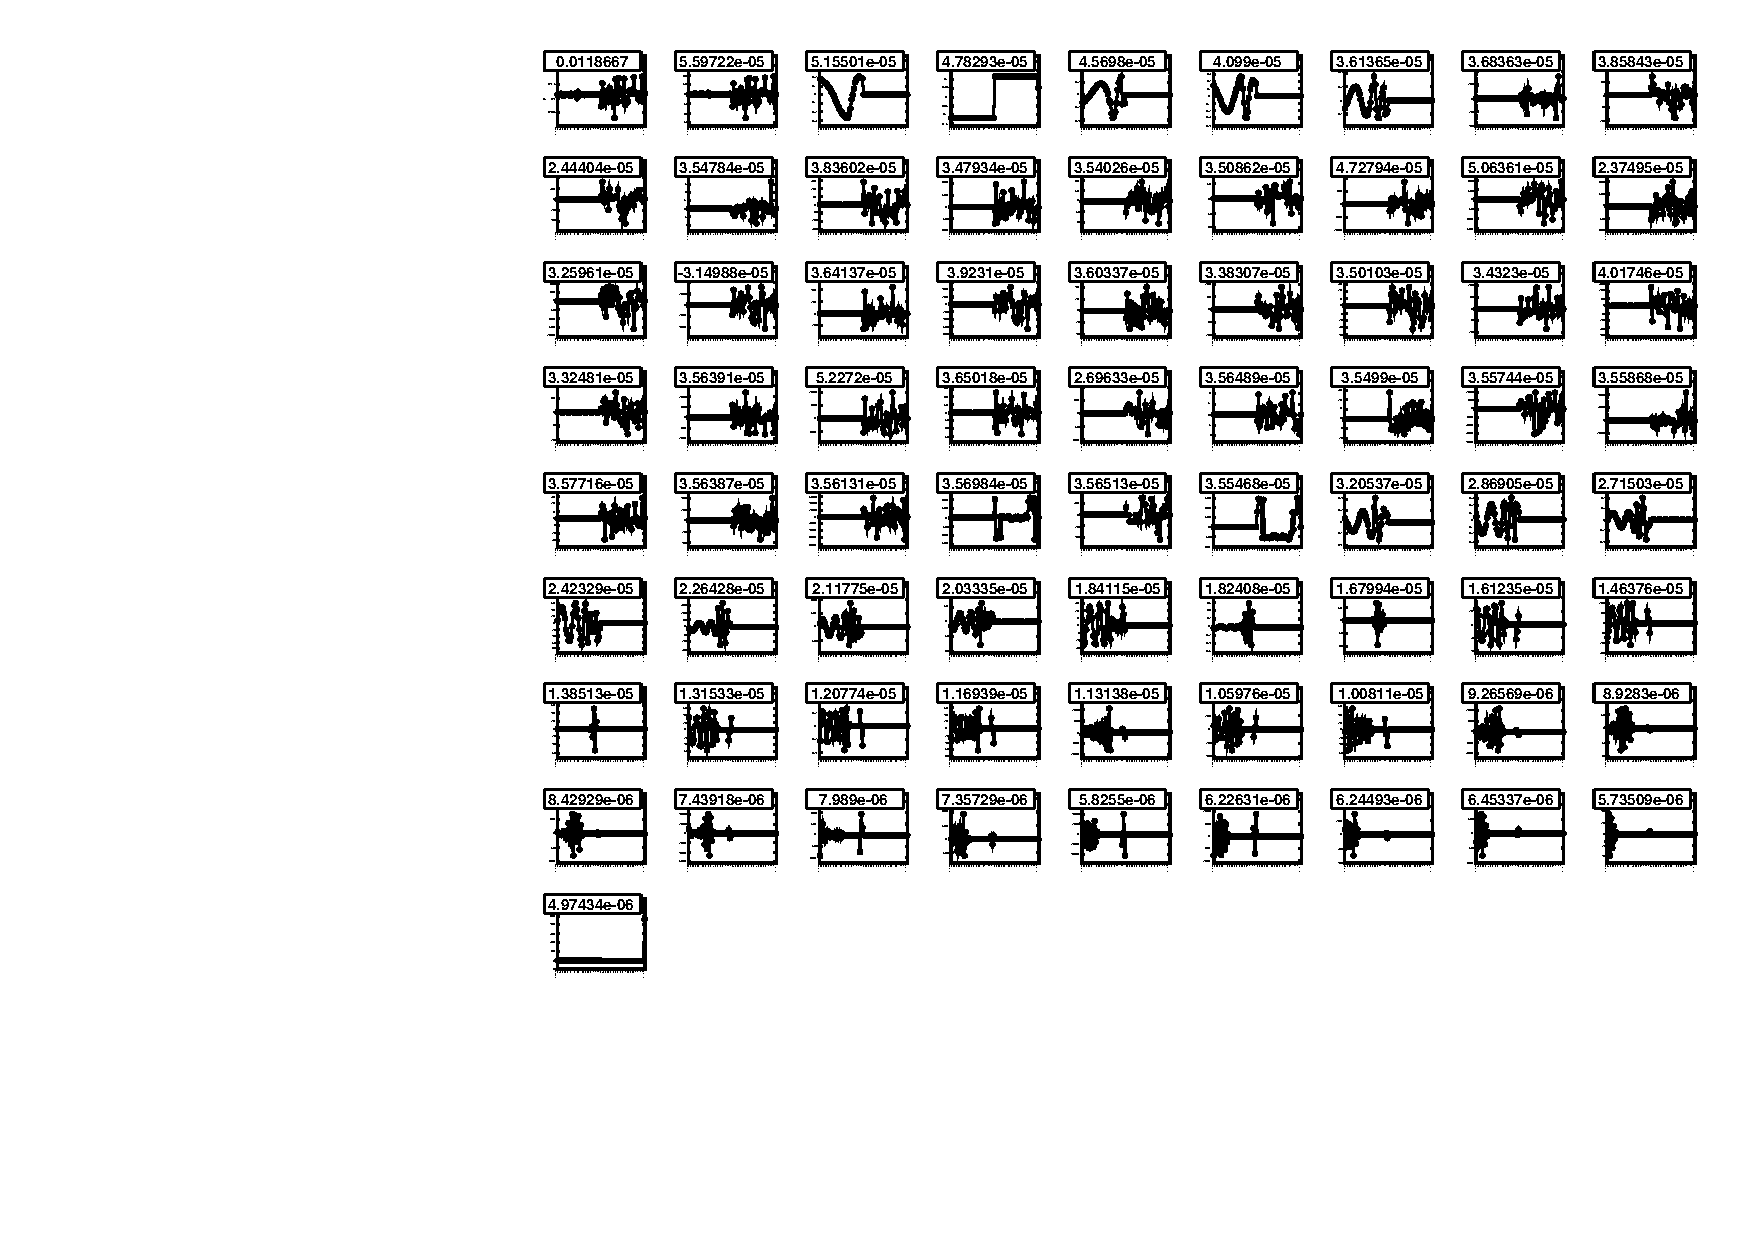
\includegraphics[width=0.9\linewidth]{newplots_errors_YEm1_x.pdf}}
\end{frame}

\begin{frame}
\frametitle{YE$-$1 $\phi_z$}

\only<1>{Convergence in $\phi_z$ positions

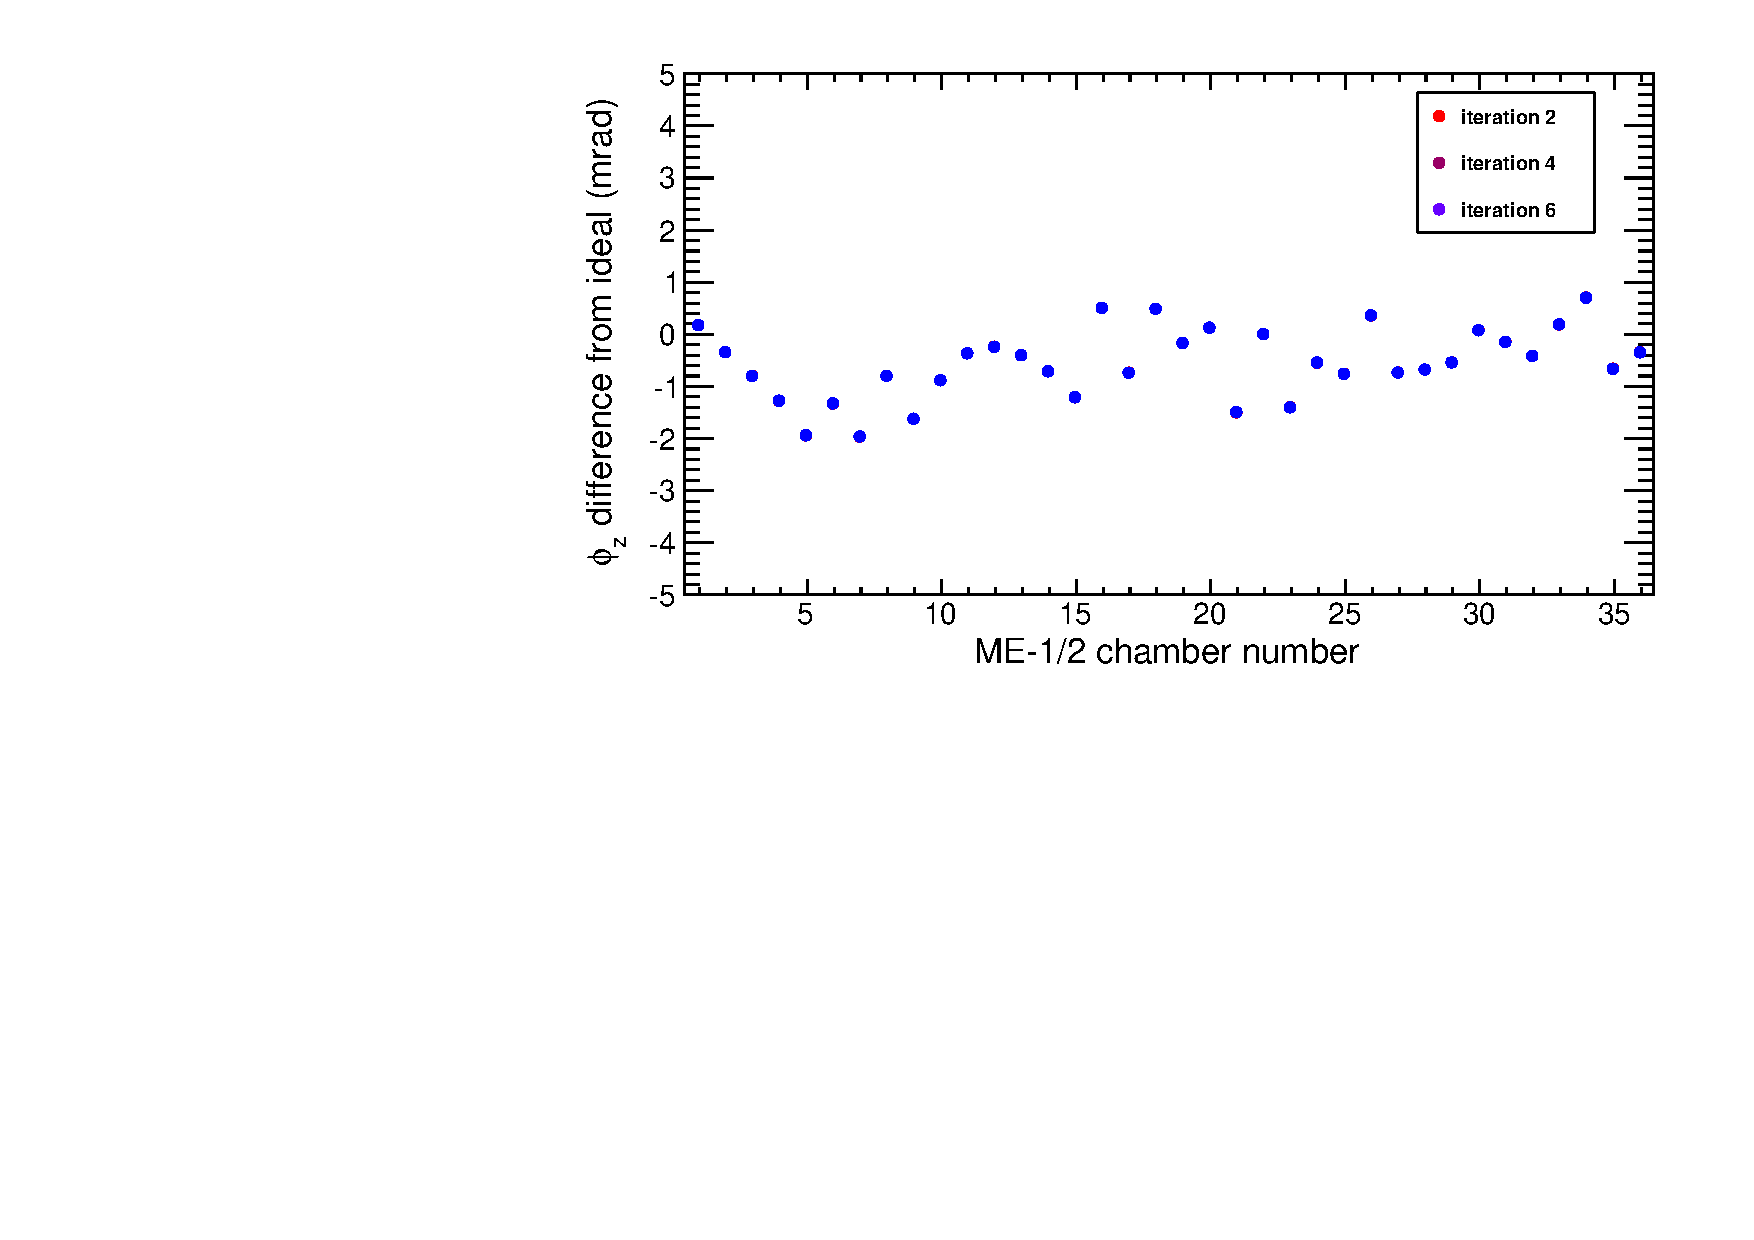
\includegraphics[width=0.6\linewidth]{newplots_convergence_mem12_phiz.pdf}

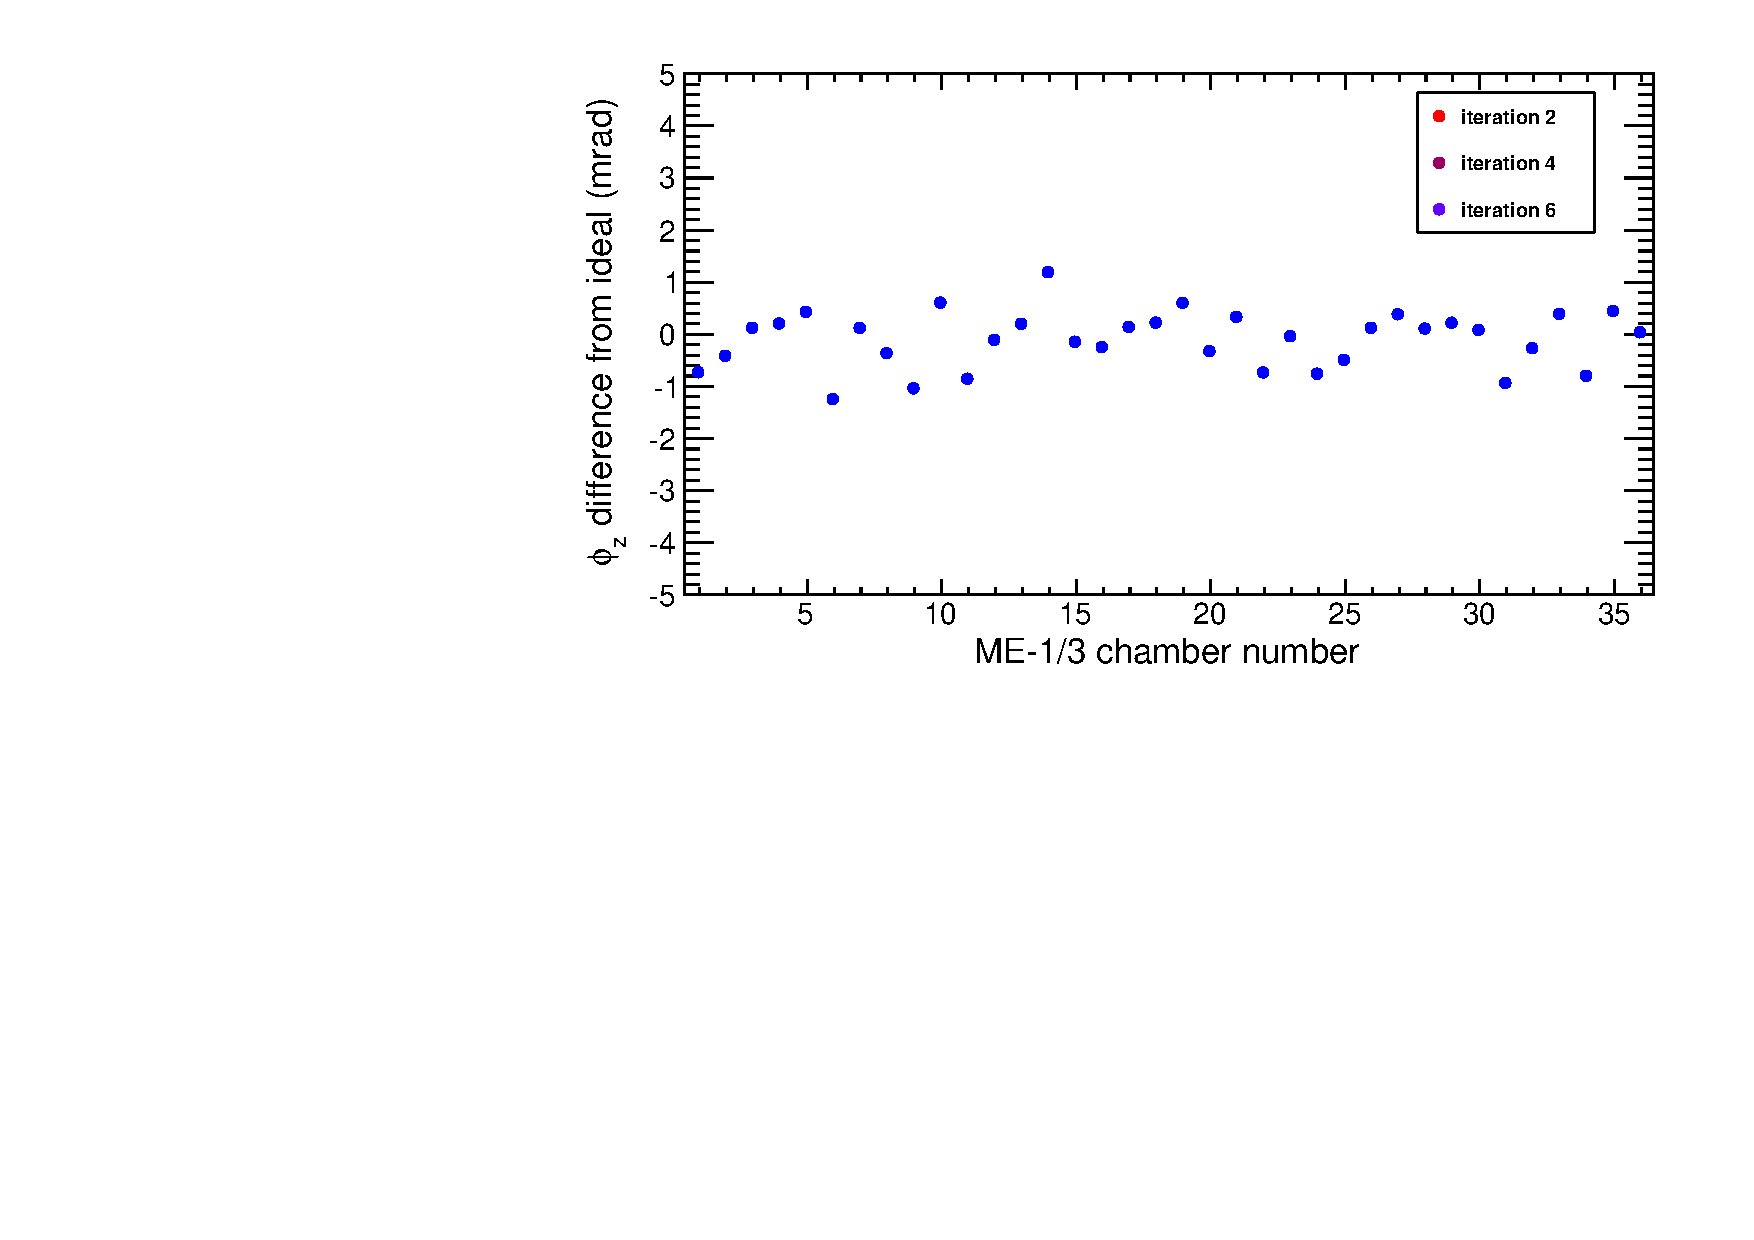
\includegraphics[width=0.6\linewidth]{newplots_convergence_mem13_phiz.pdf}}
\only<2>{Fit residuals in $\phi_z$ (not track residuals): no BH in ME$-$1/3 (green)

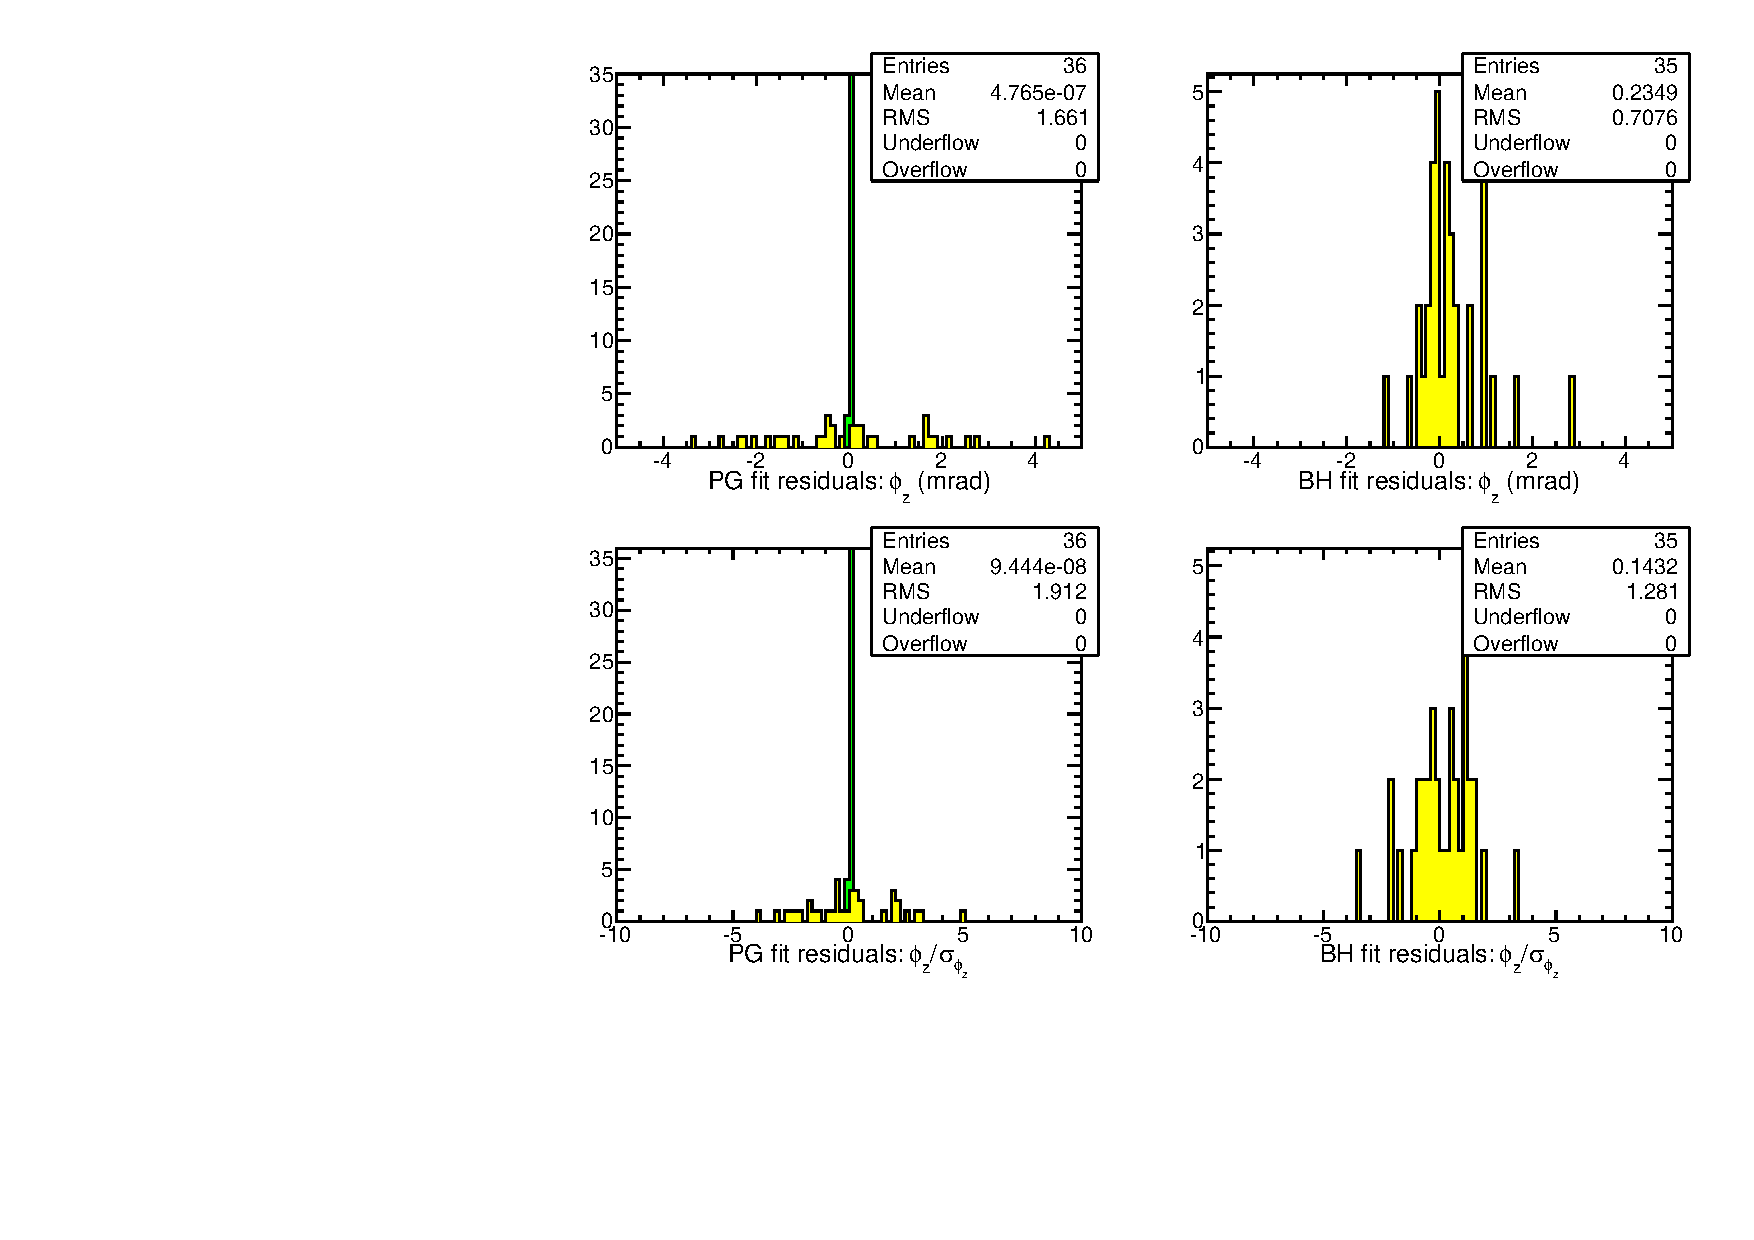
\includegraphics[width=0.9\linewidth]{newplots_fitresiduals_YEm1_phiz.pdf}}
\only<3>{Numbers in boxes are $\phi_z$ angle uncertainty in each mode in rad

First 1 is completely undetermined (uncertainty is meaningless)

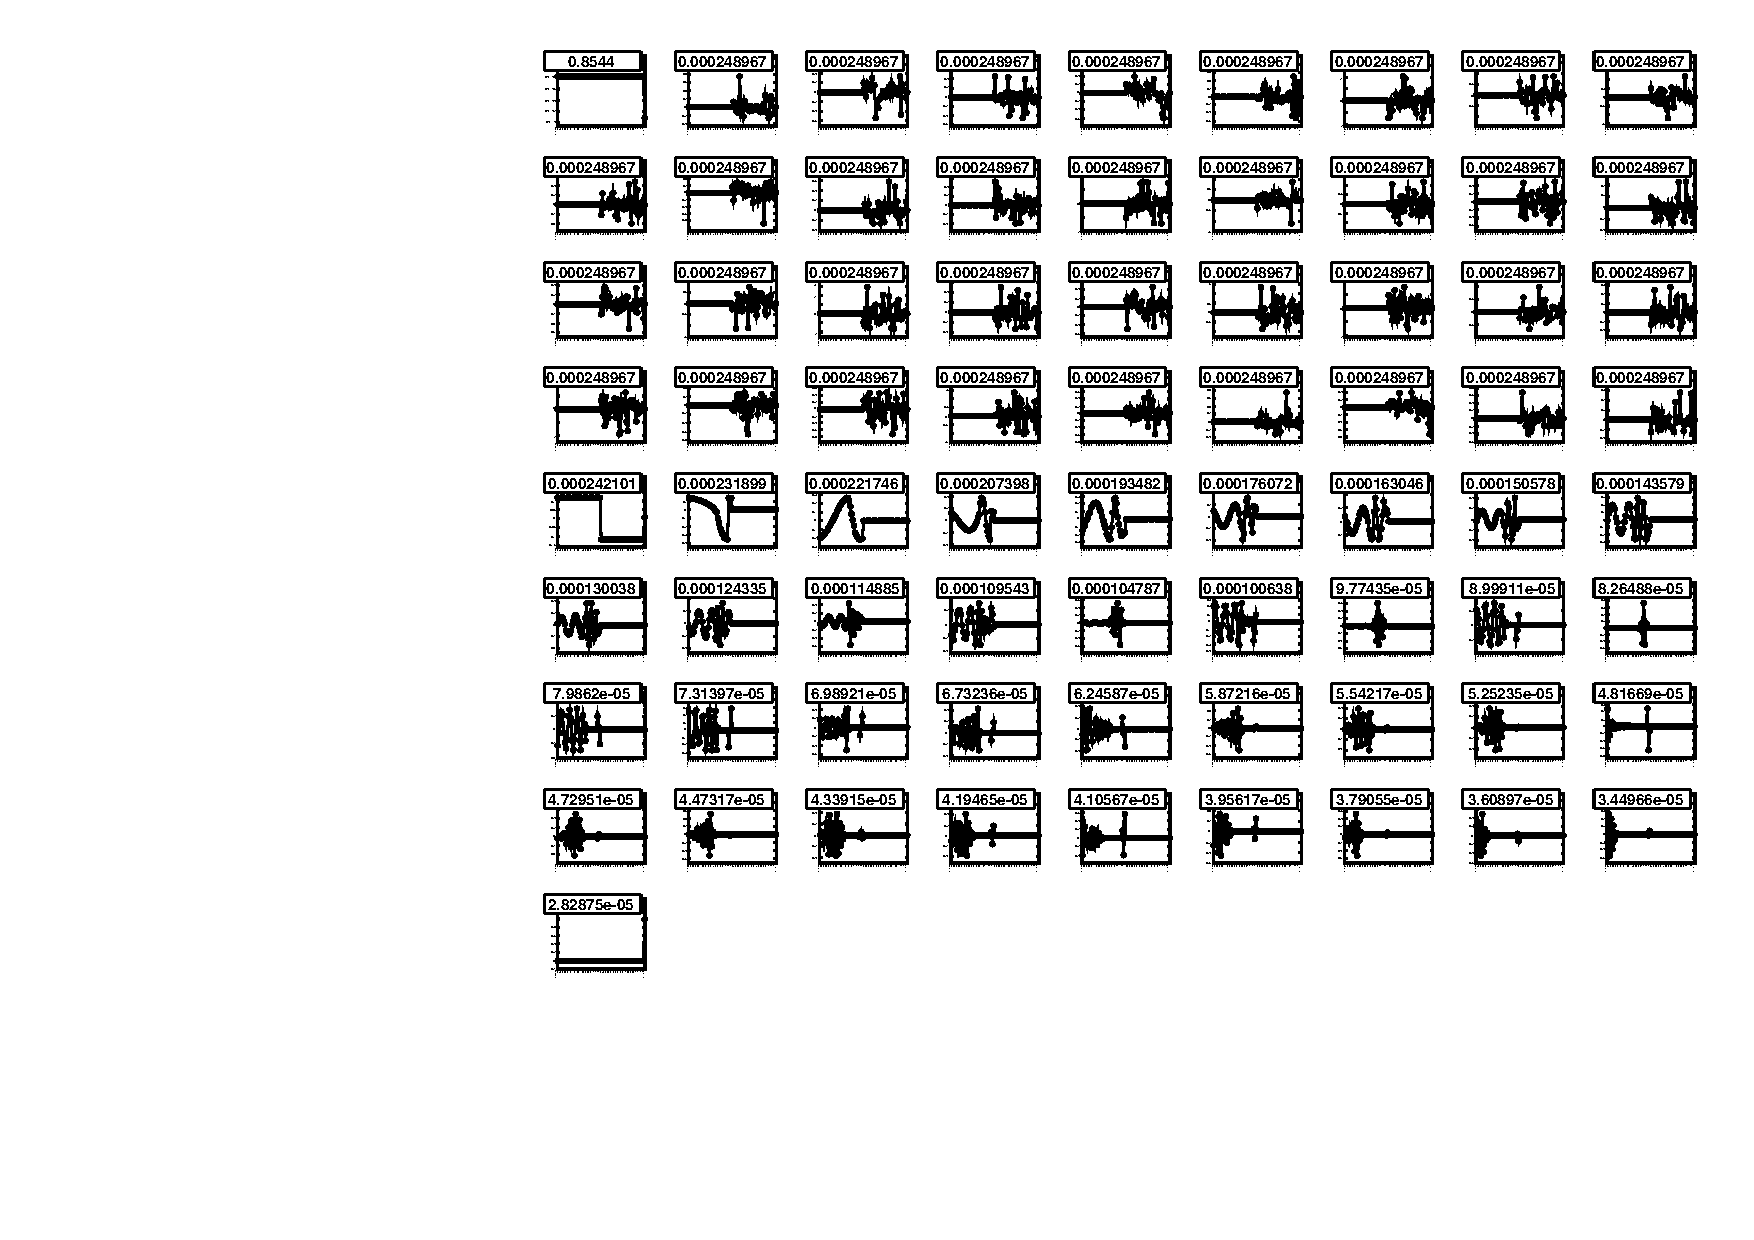
\includegraphics[width=0.9\linewidth]{newplots_errors_YEm1_phiz.pdf}}
\end{frame}

\begin{frame}
\frametitle{YE$+$2 $r\phi$}

\only<1>{Convergence in $r\phi$ positions

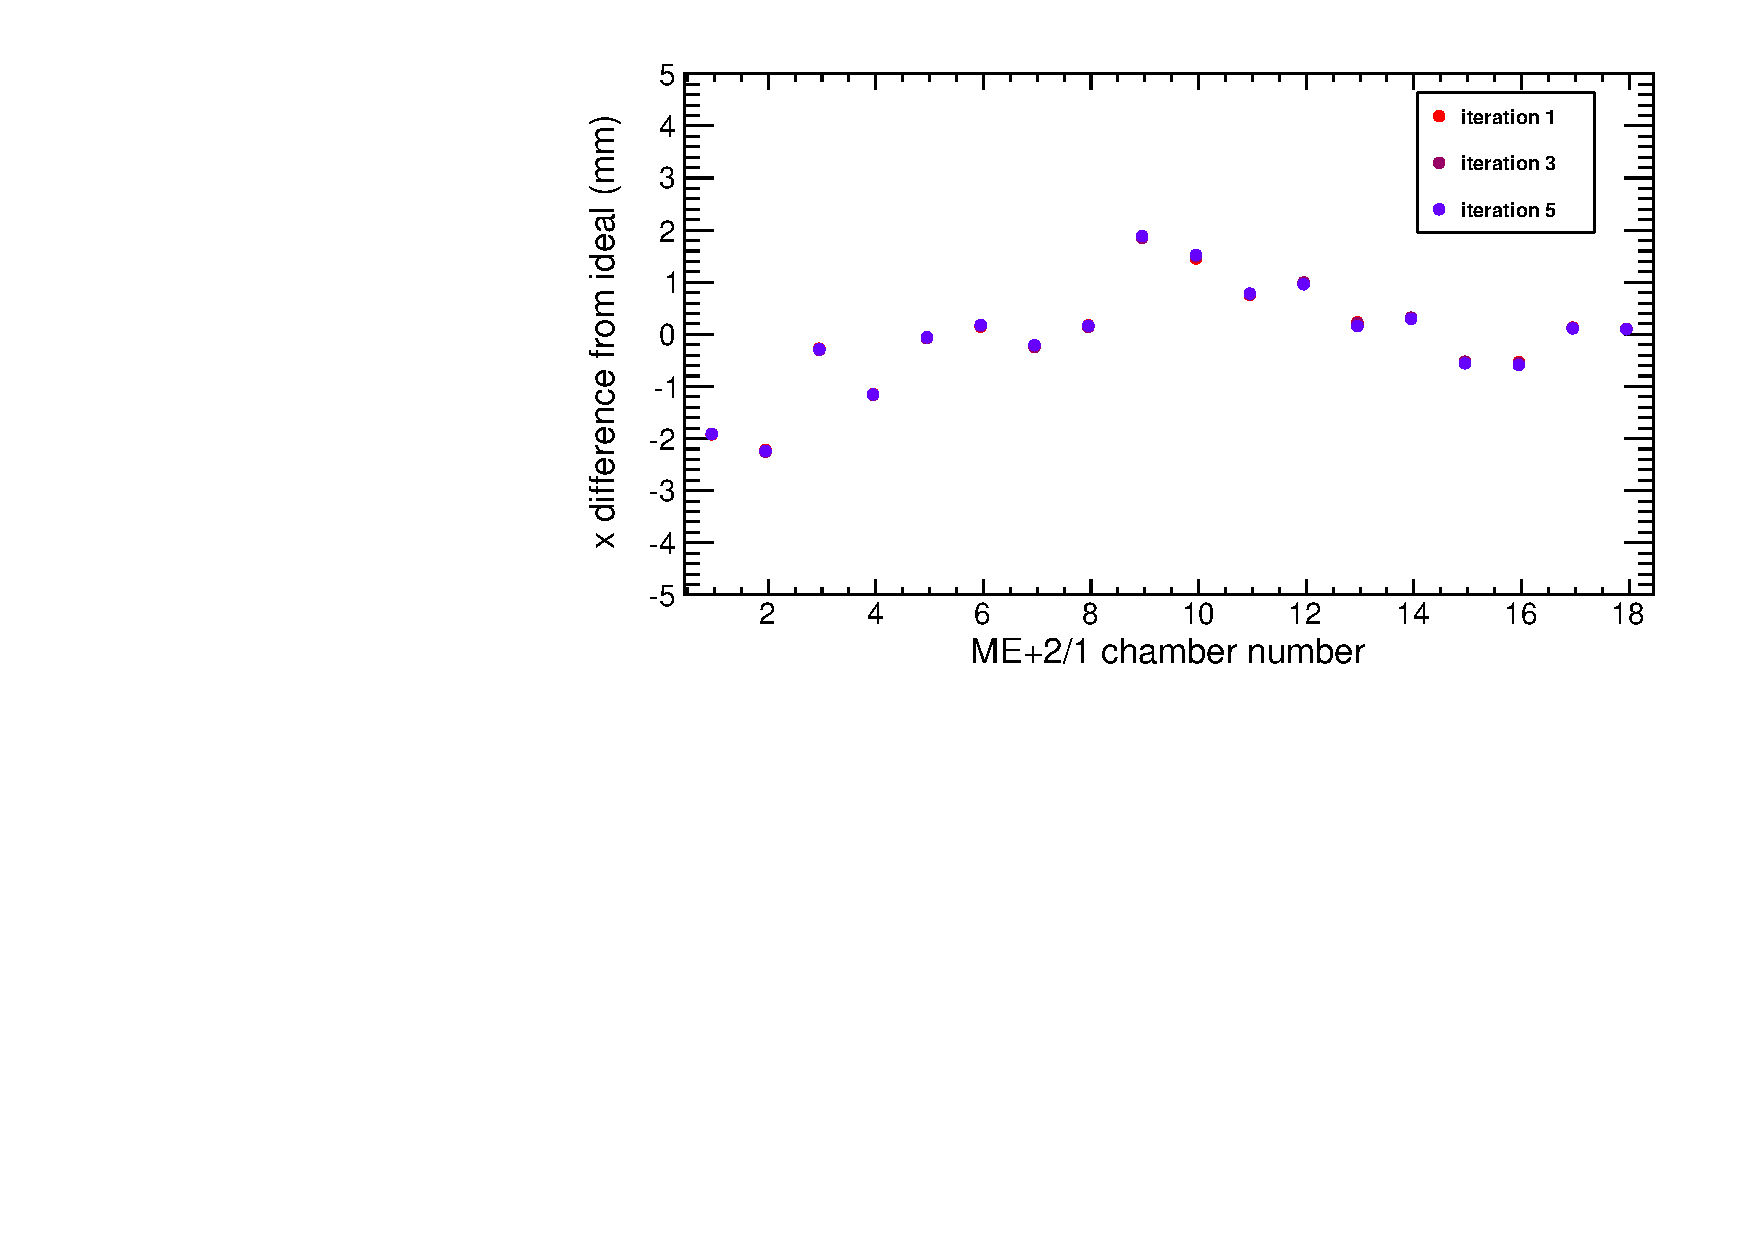
\includegraphics[width=0.6\linewidth]{newplots_convergence_mep21_x.pdf}

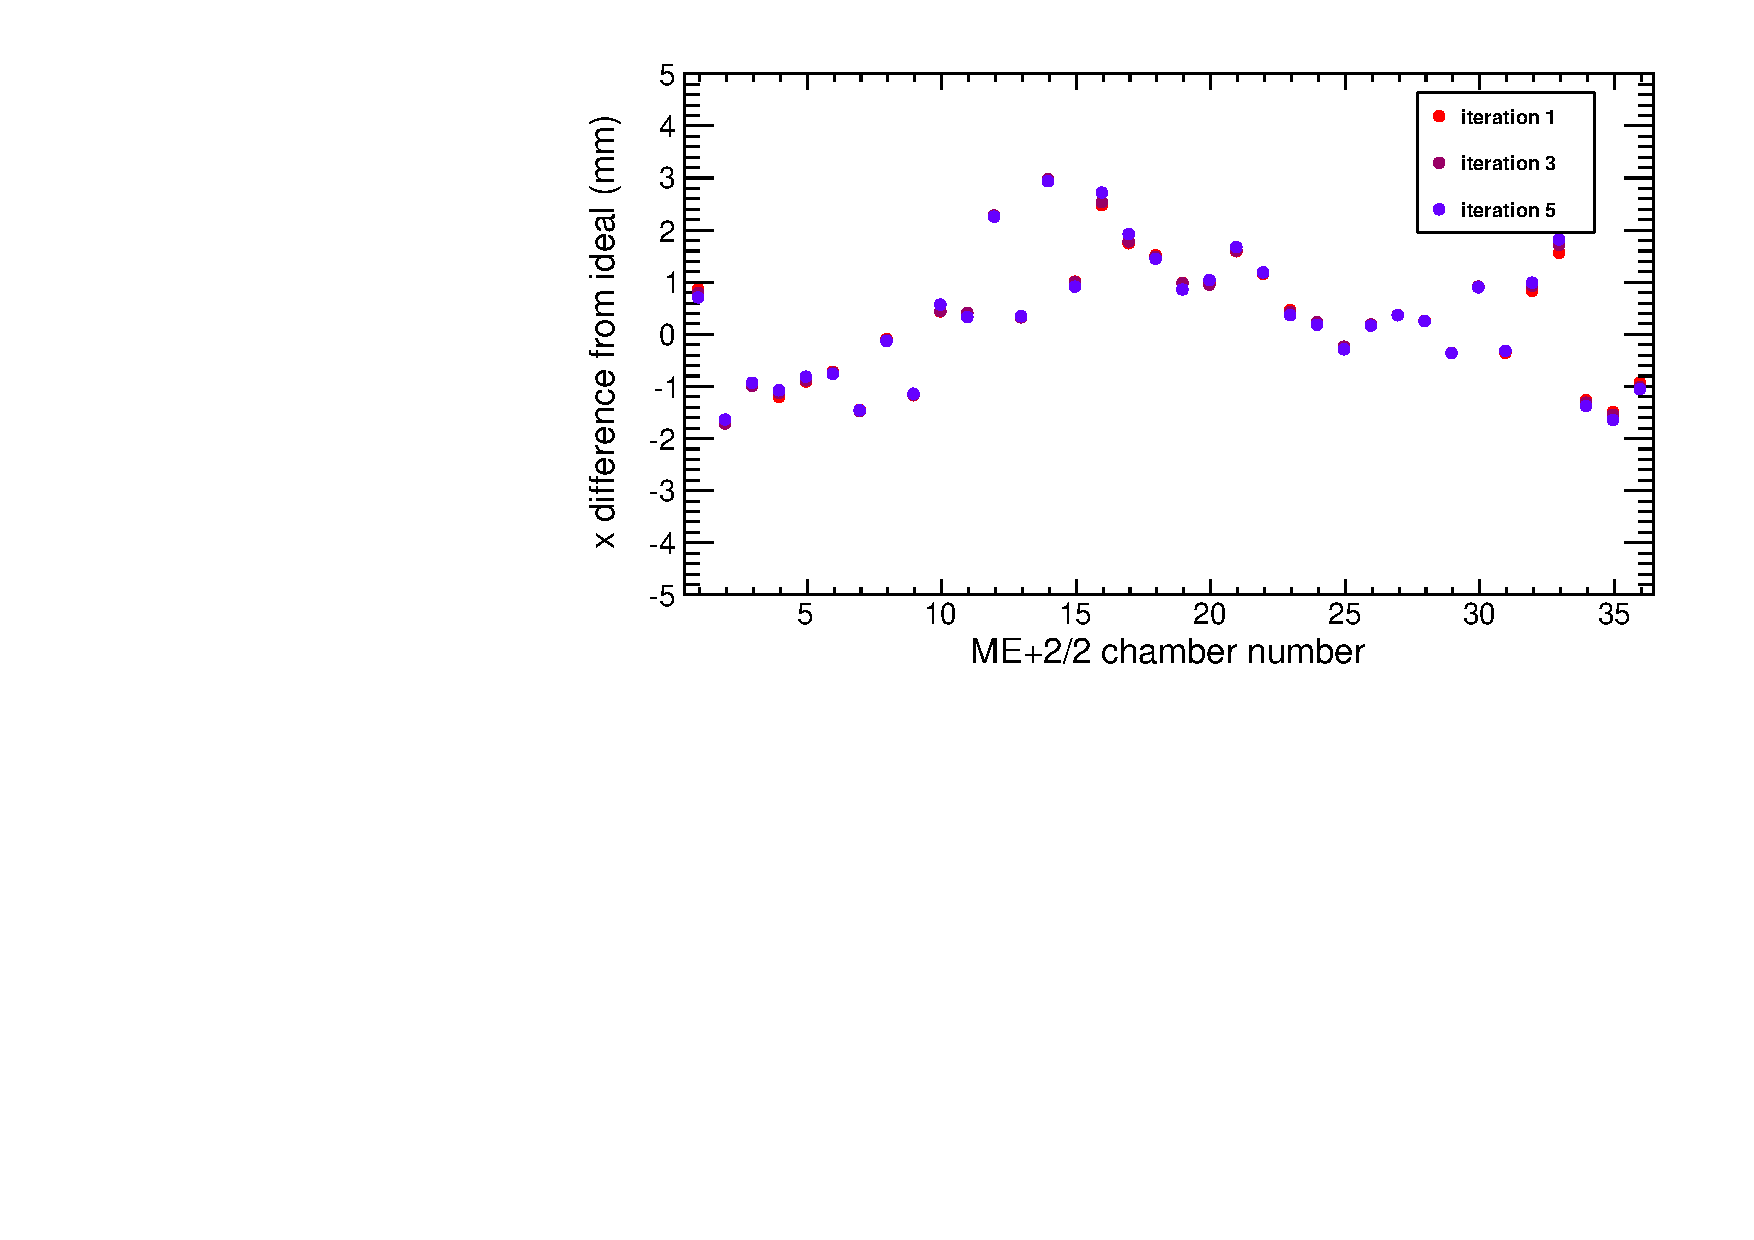
\includegraphics[width=0.6\linewidth]{newplots_convergence_mep22_x.pdf}}
\only<2>{Convergence in $r\phi$ positions

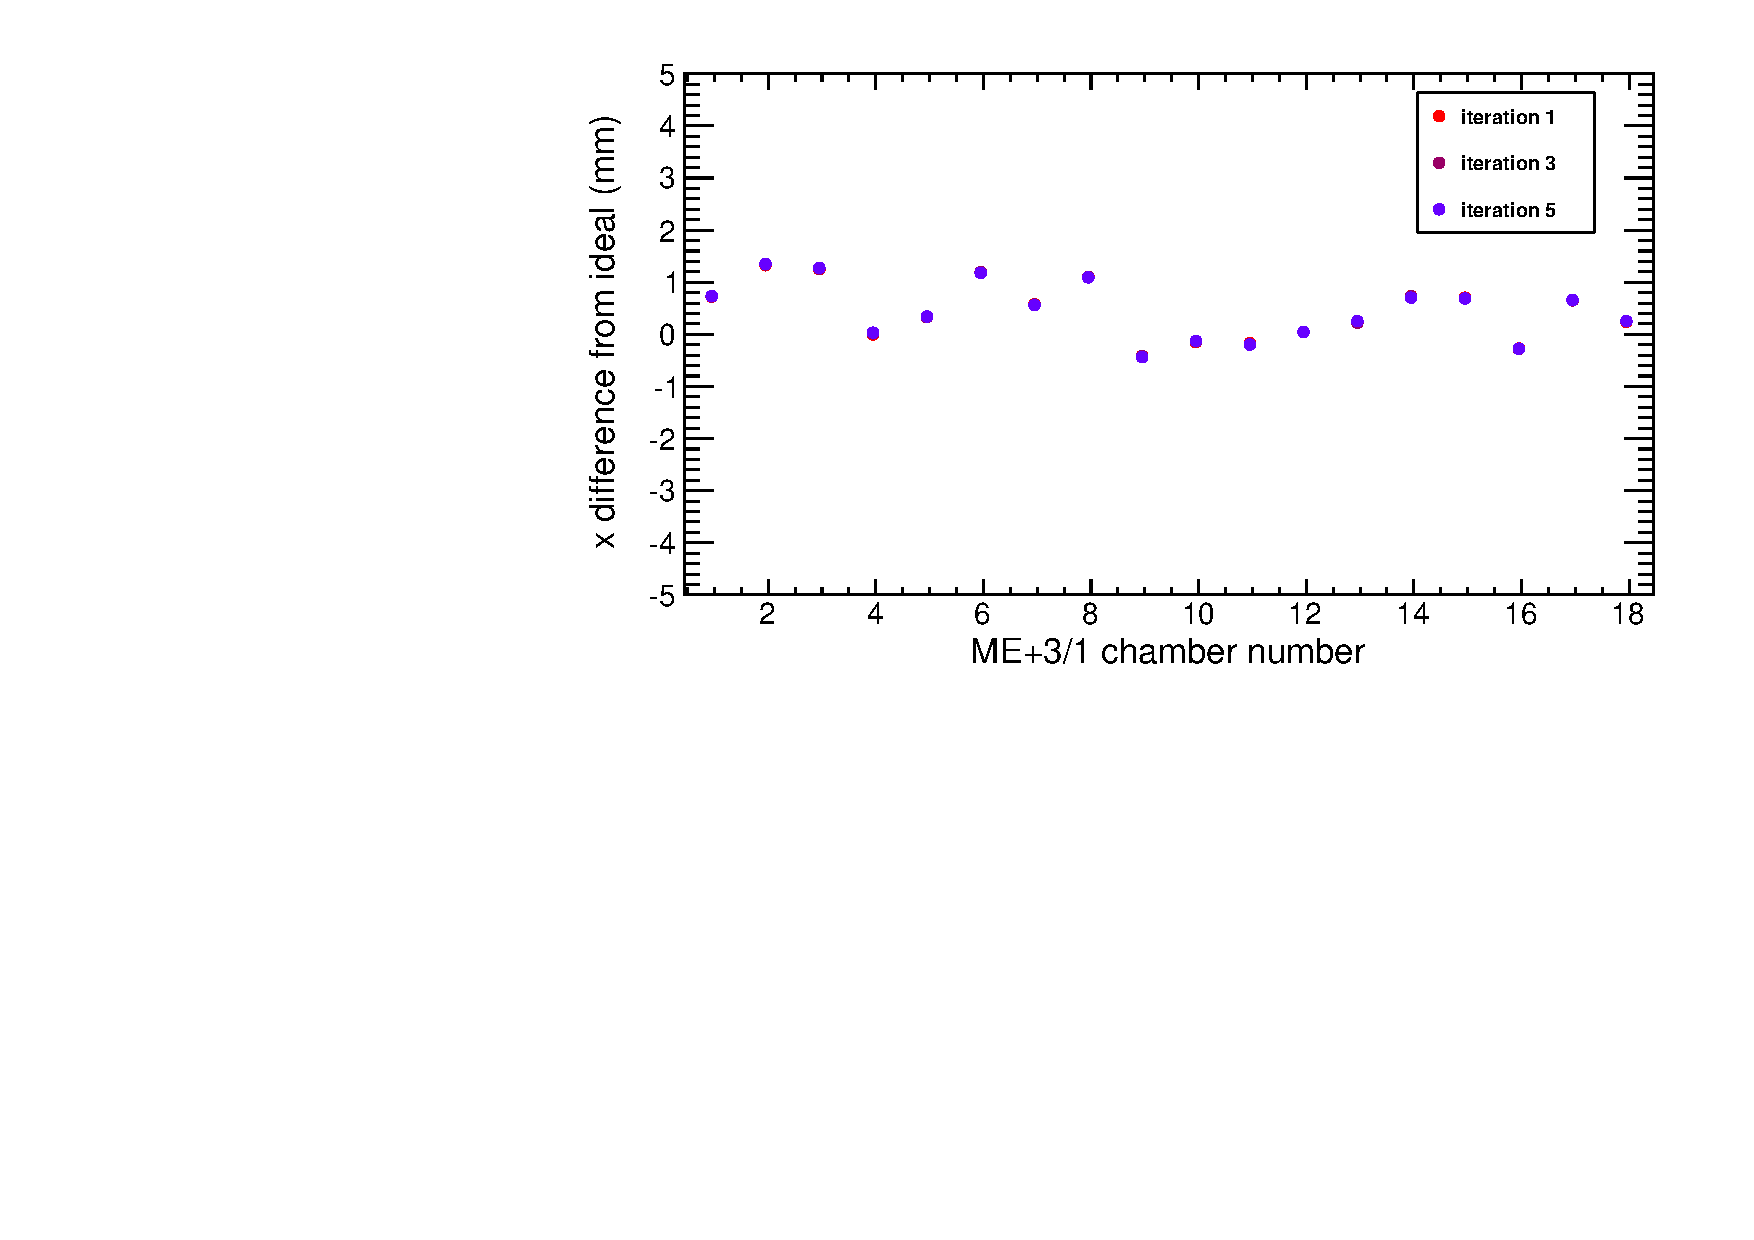
\includegraphics[width=0.6\linewidth]{newplots_convergence_mep31_x.pdf}

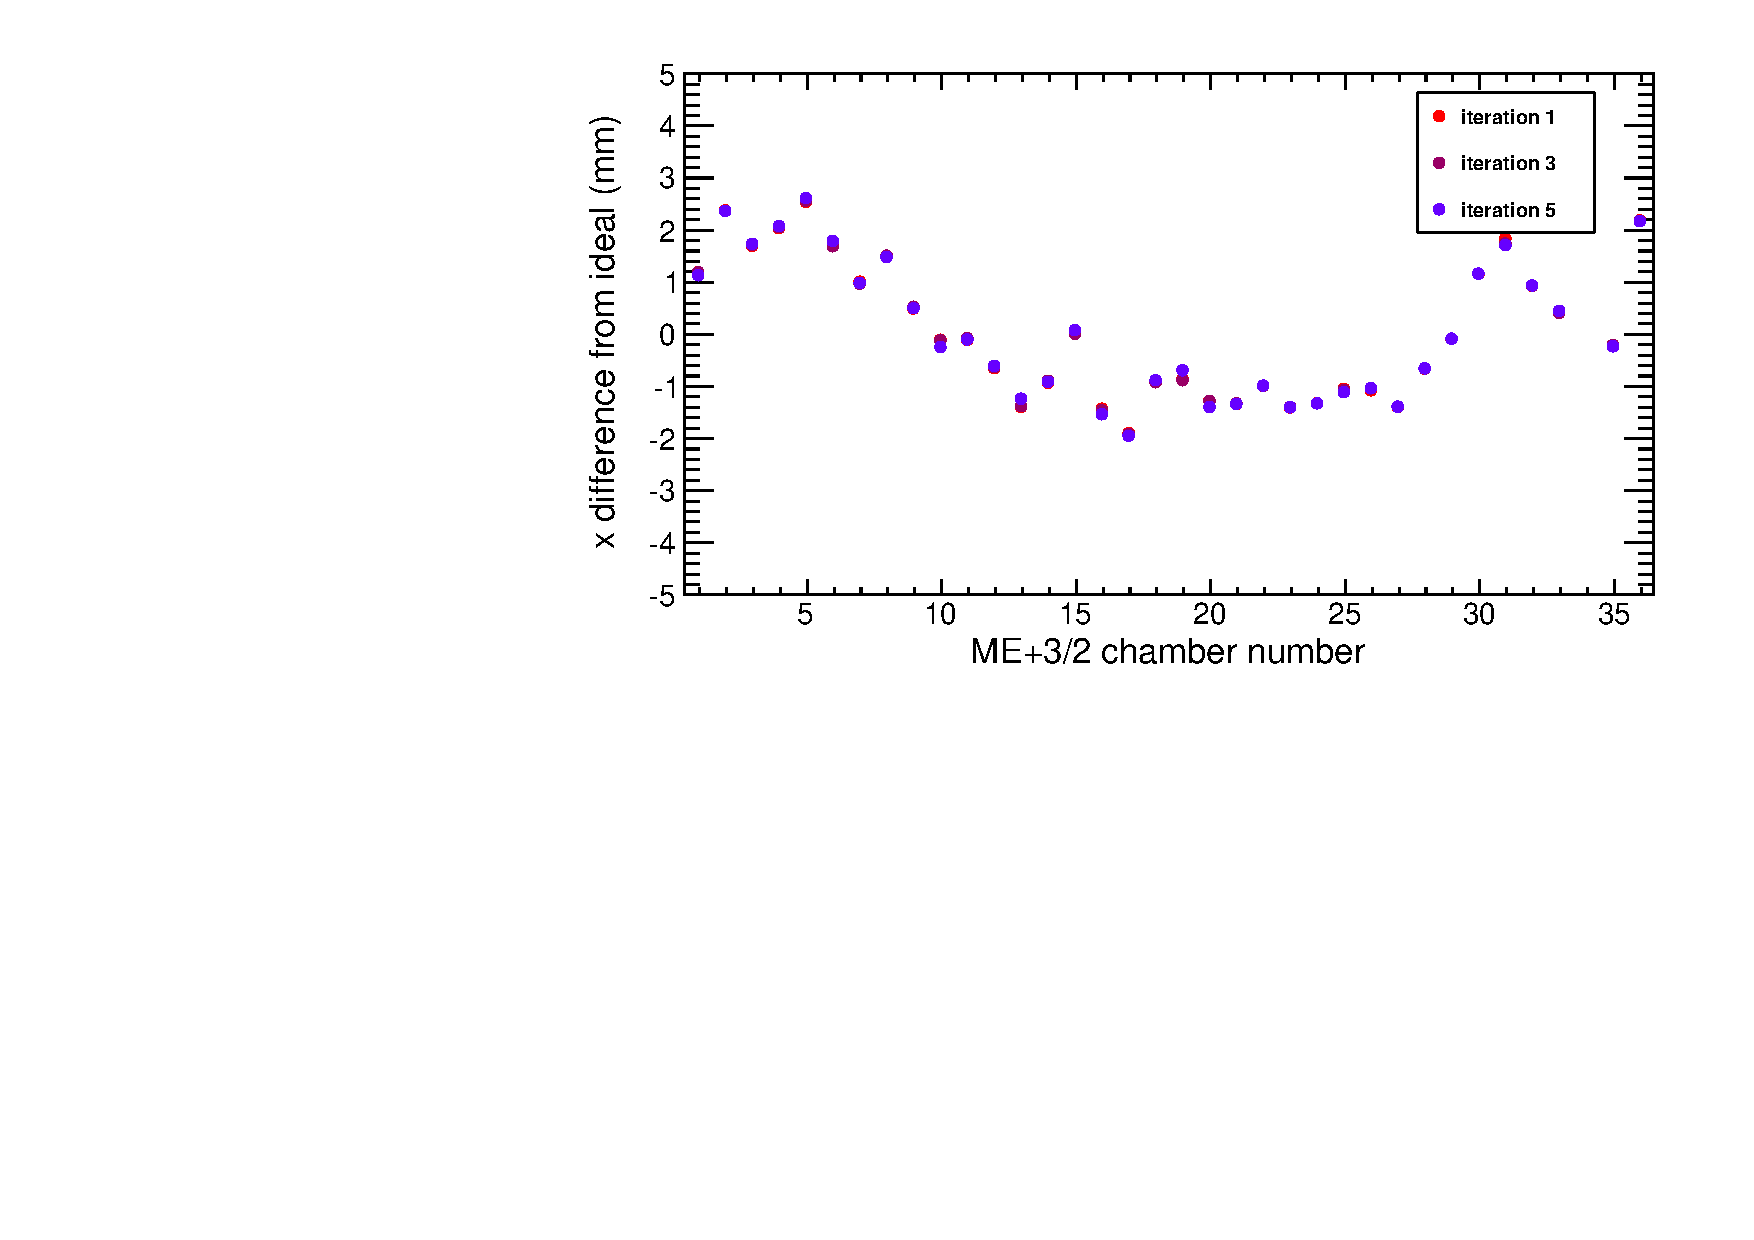
\includegraphics[width=0.6\linewidth]{newplots_convergence_mep32_x.pdf}}
\only<3>{Fit residuals in $r\phi$ (not track residuals)

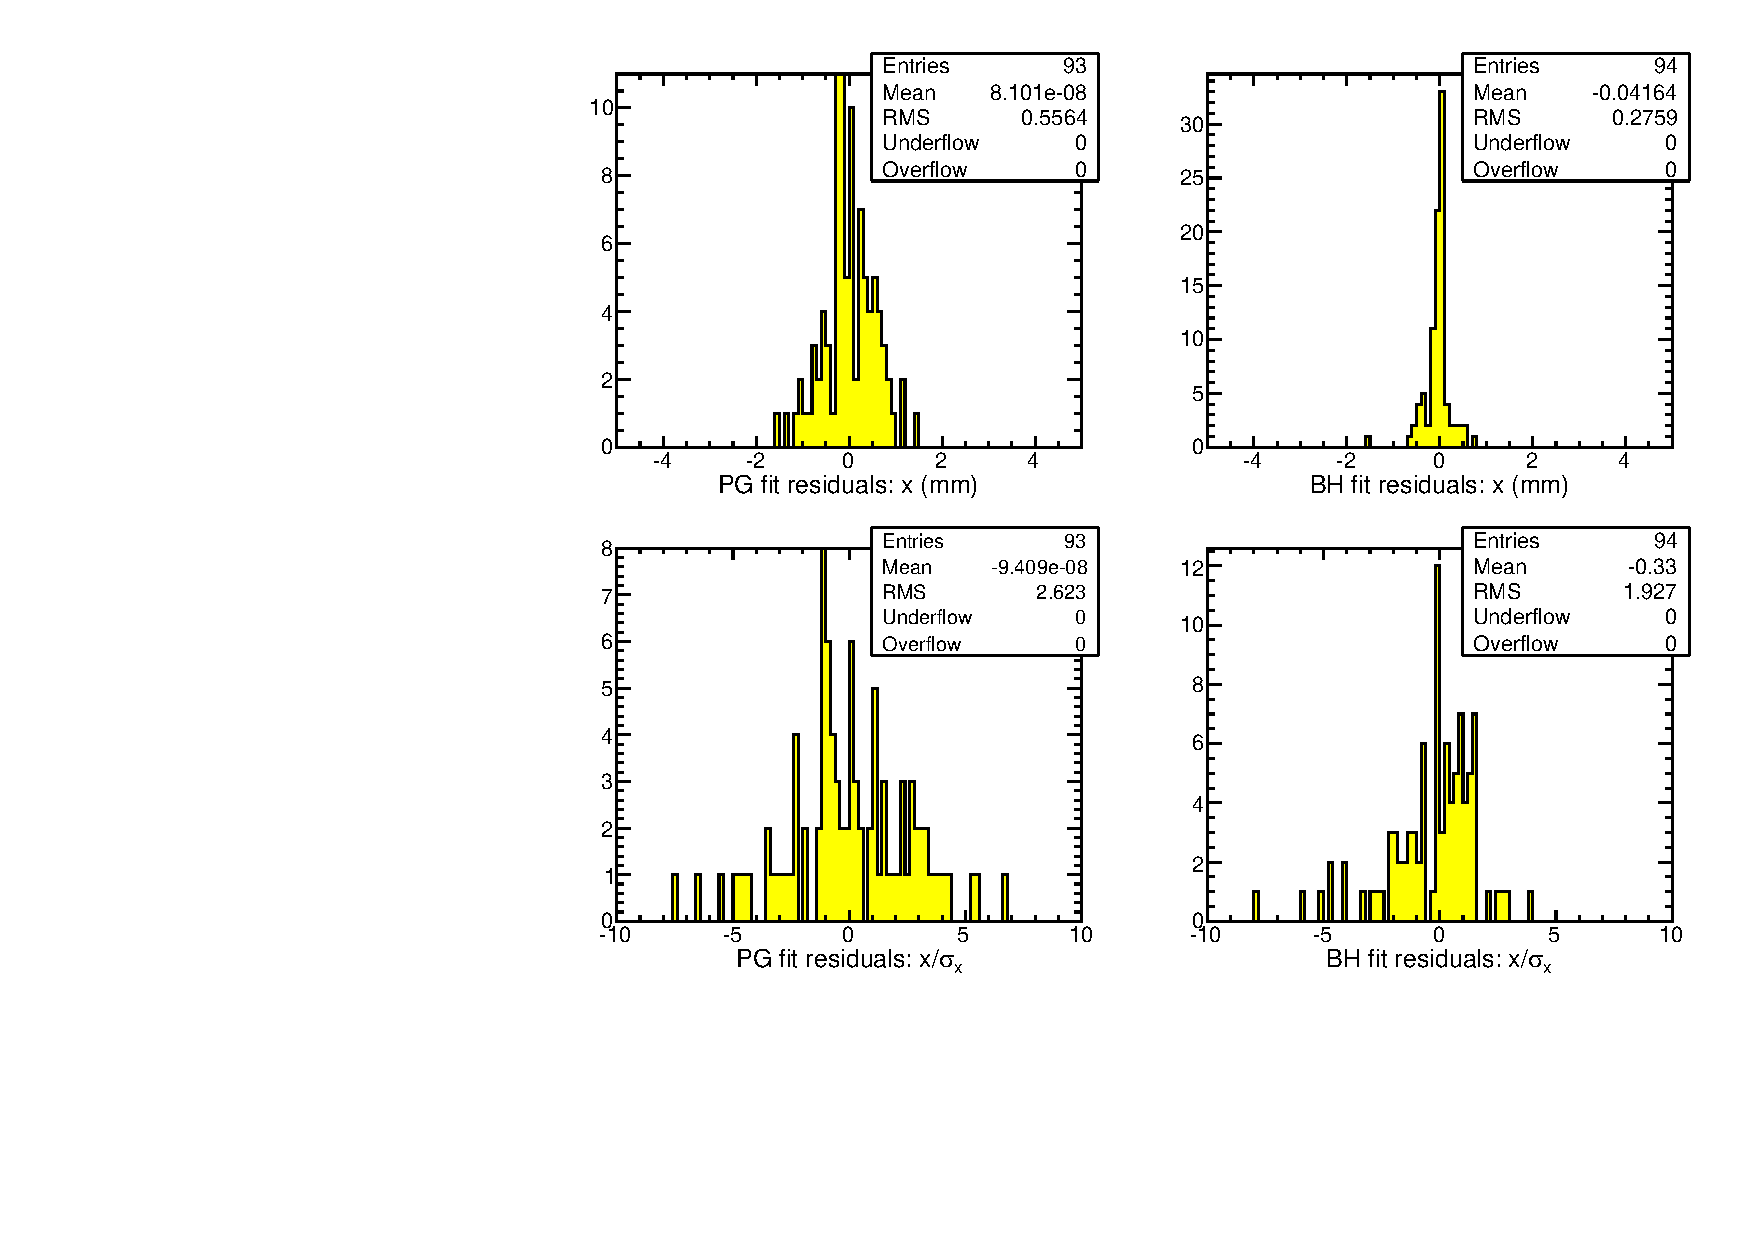
\includegraphics[width=0.9\linewidth]{newplots_fitresiduals_YEp2_x.pdf}}
\only<4>{Numbers in boxes are $\phi$ position uncertainty in each mode in rad

First 2 are completely undetermined (uncertainty is meaningless)

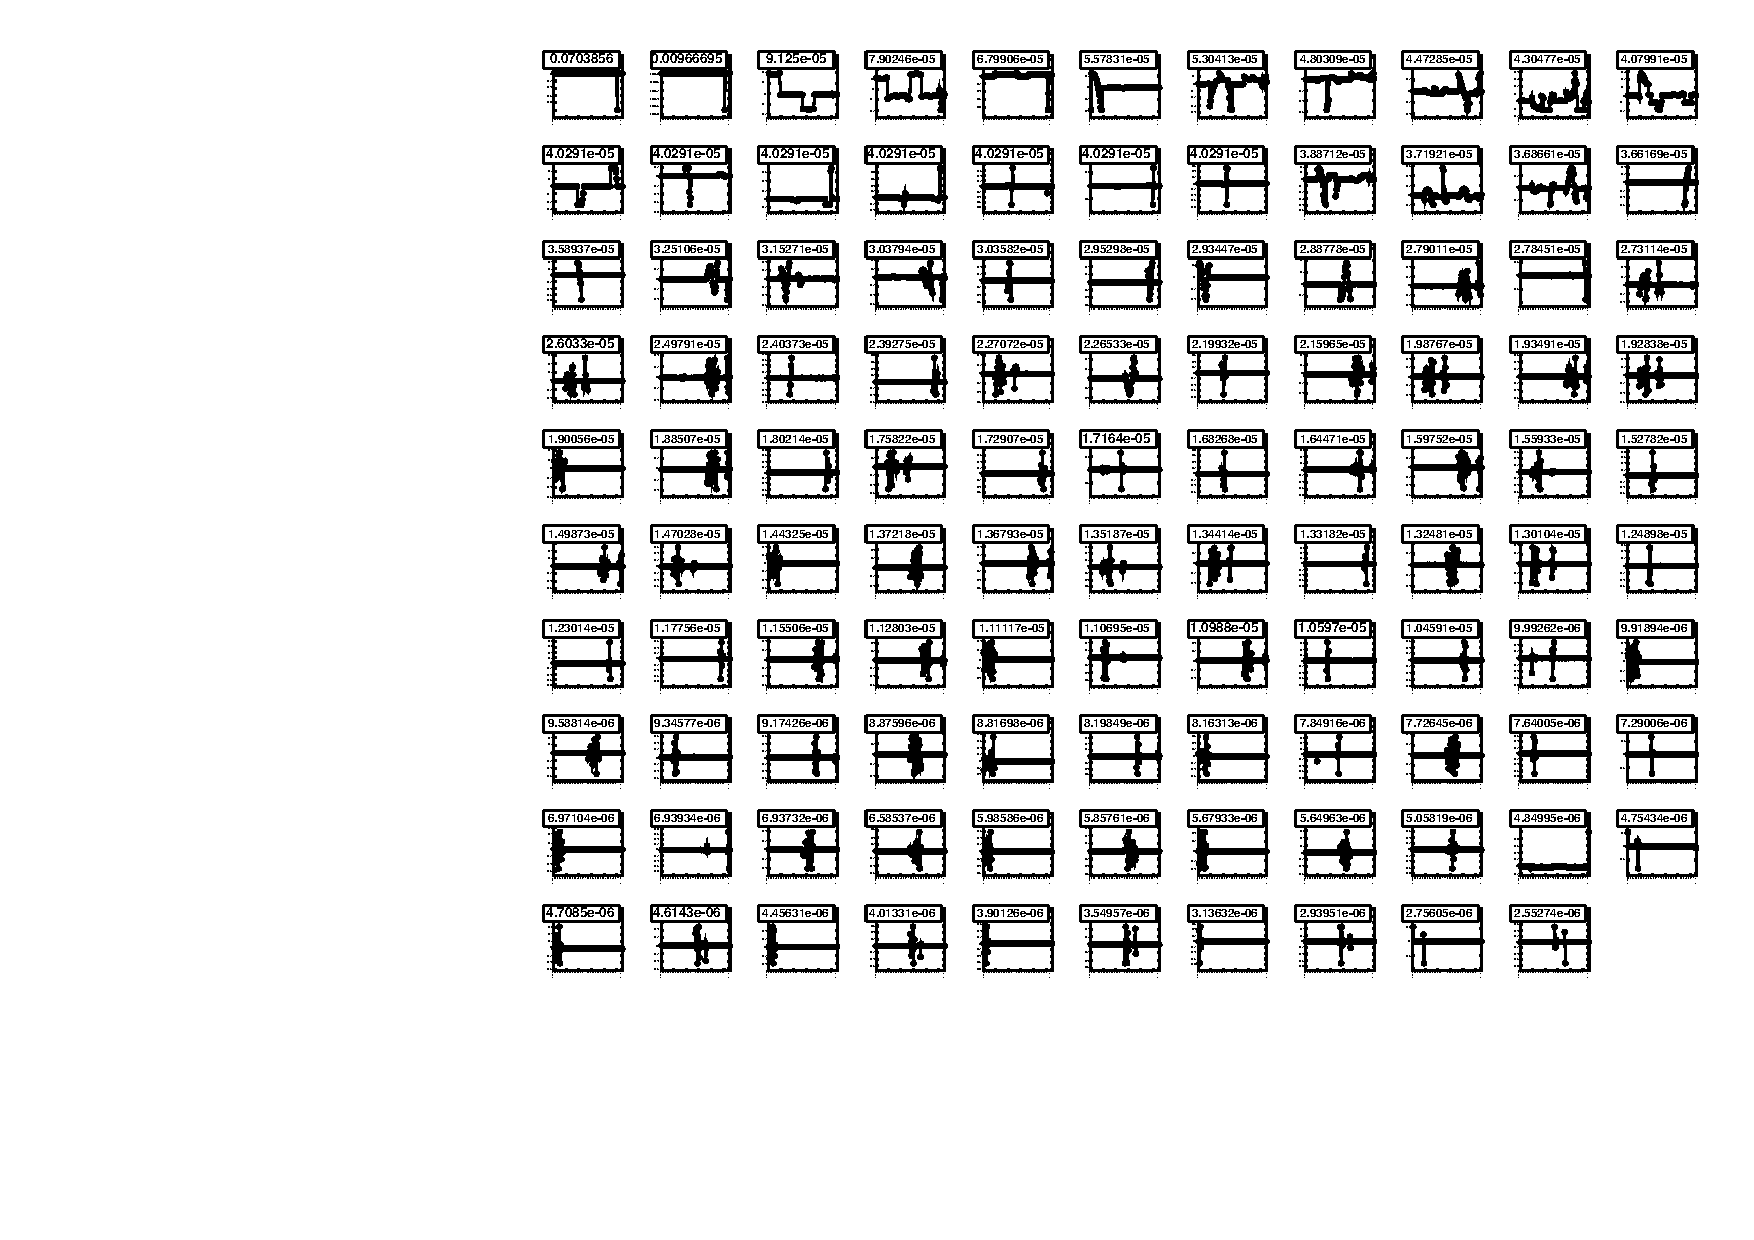
\includegraphics[width=0.9\linewidth]{newplots_errors_YEp2_x.pdf}}
\end{frame}

\begin{frame}
\frametitle{YE$+$2 $\phi_z$}

\only<1>{Convergence in $\phi_z$ positions

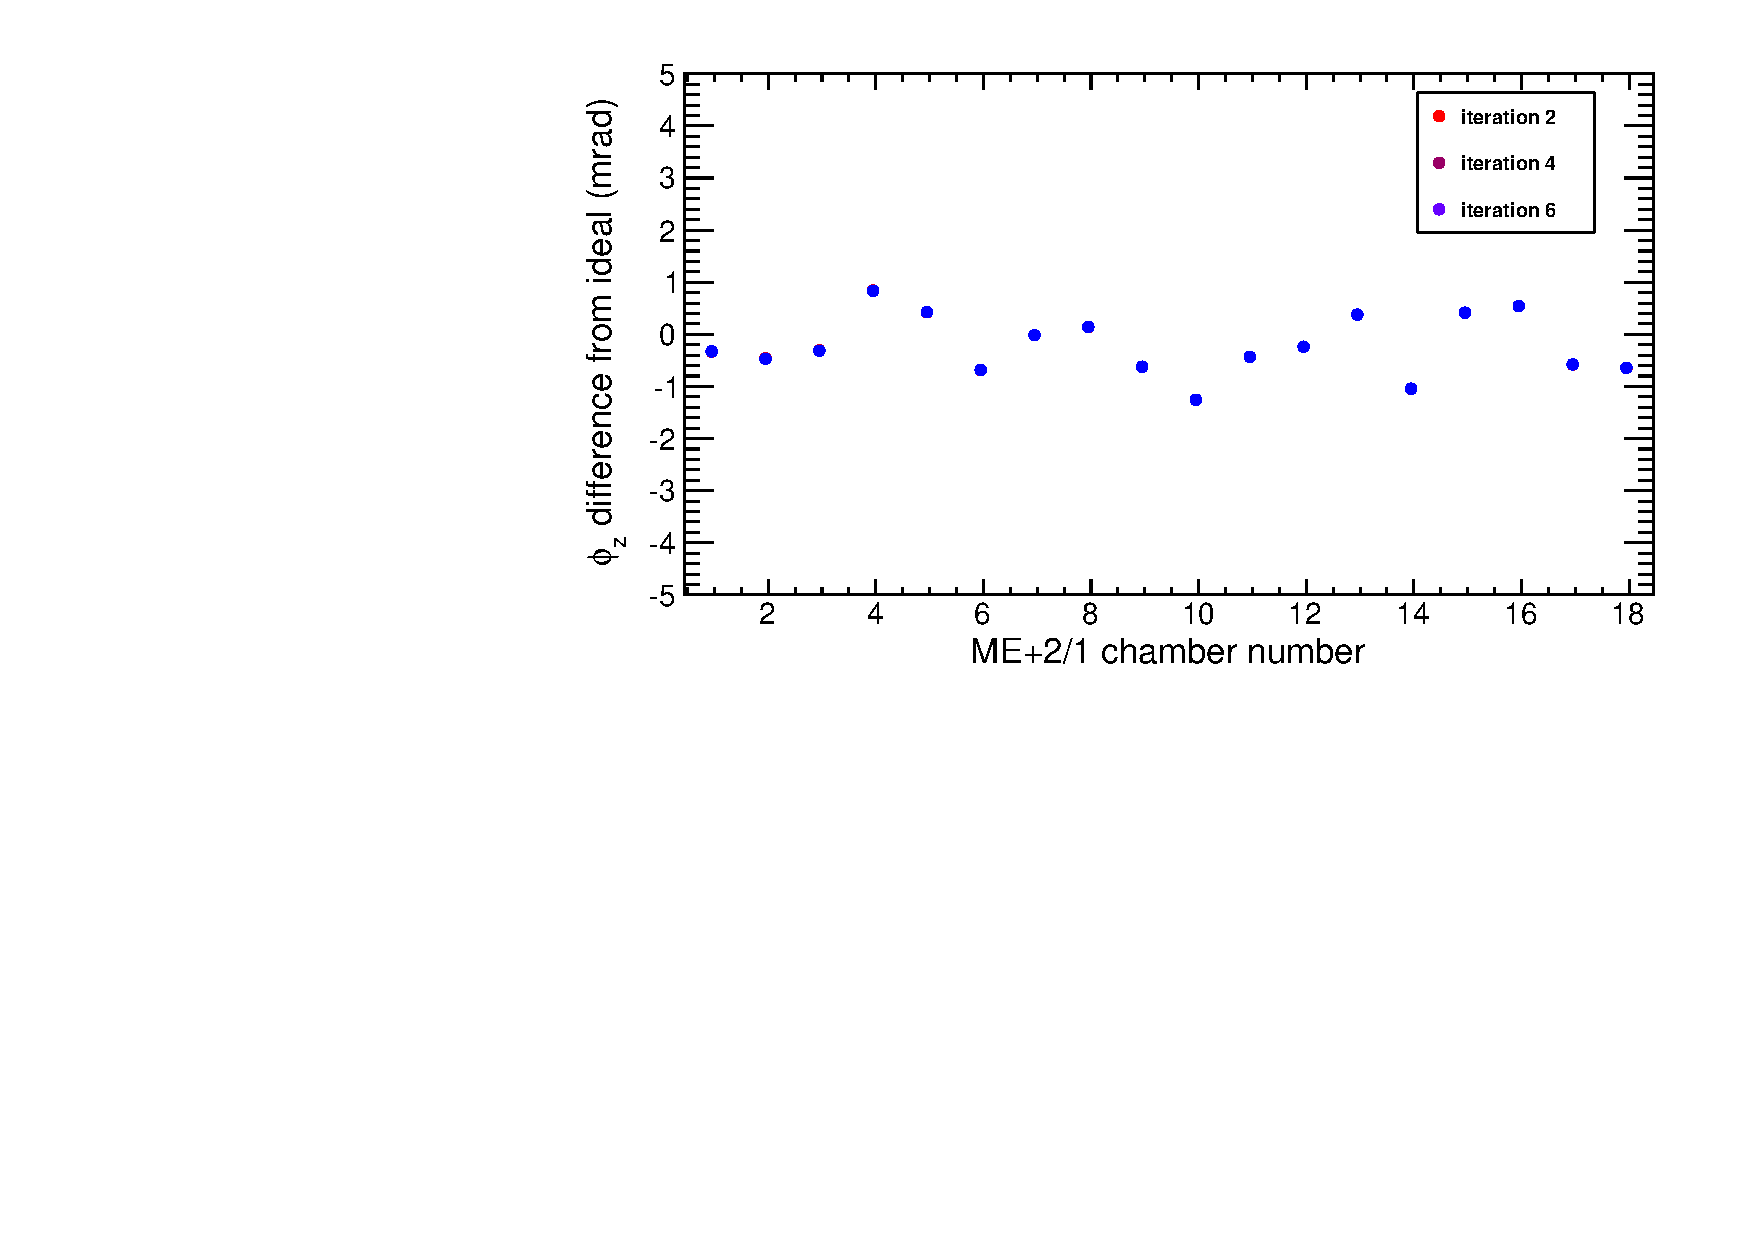
\includegraphics[width=0.6\linewidth]{newplots_convergence_mep21_phiz.pdf}

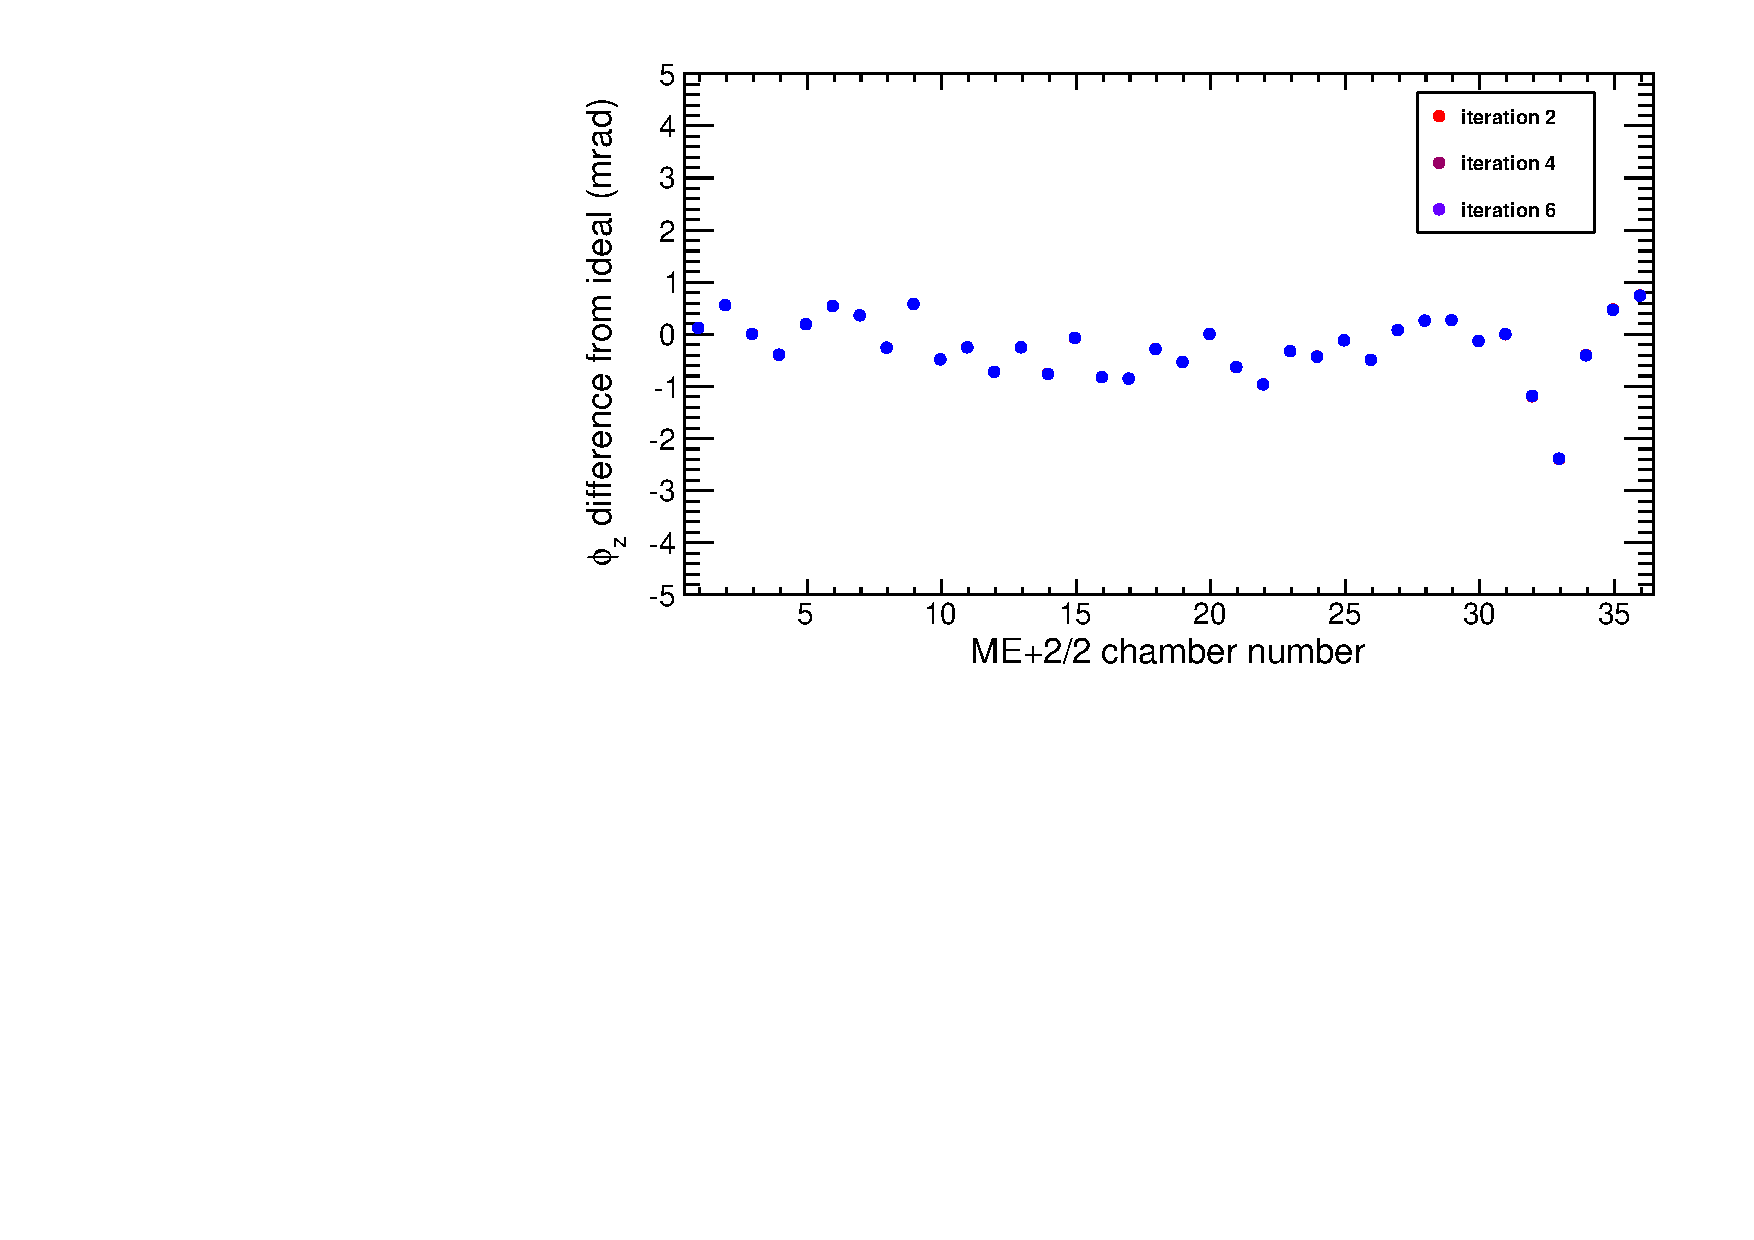
\includegraphics[width=0.6\linewidth]{newplots_convergence_mep22_phiz.pdf}}
\only<2>{Convergence in $\phi_z$ positions

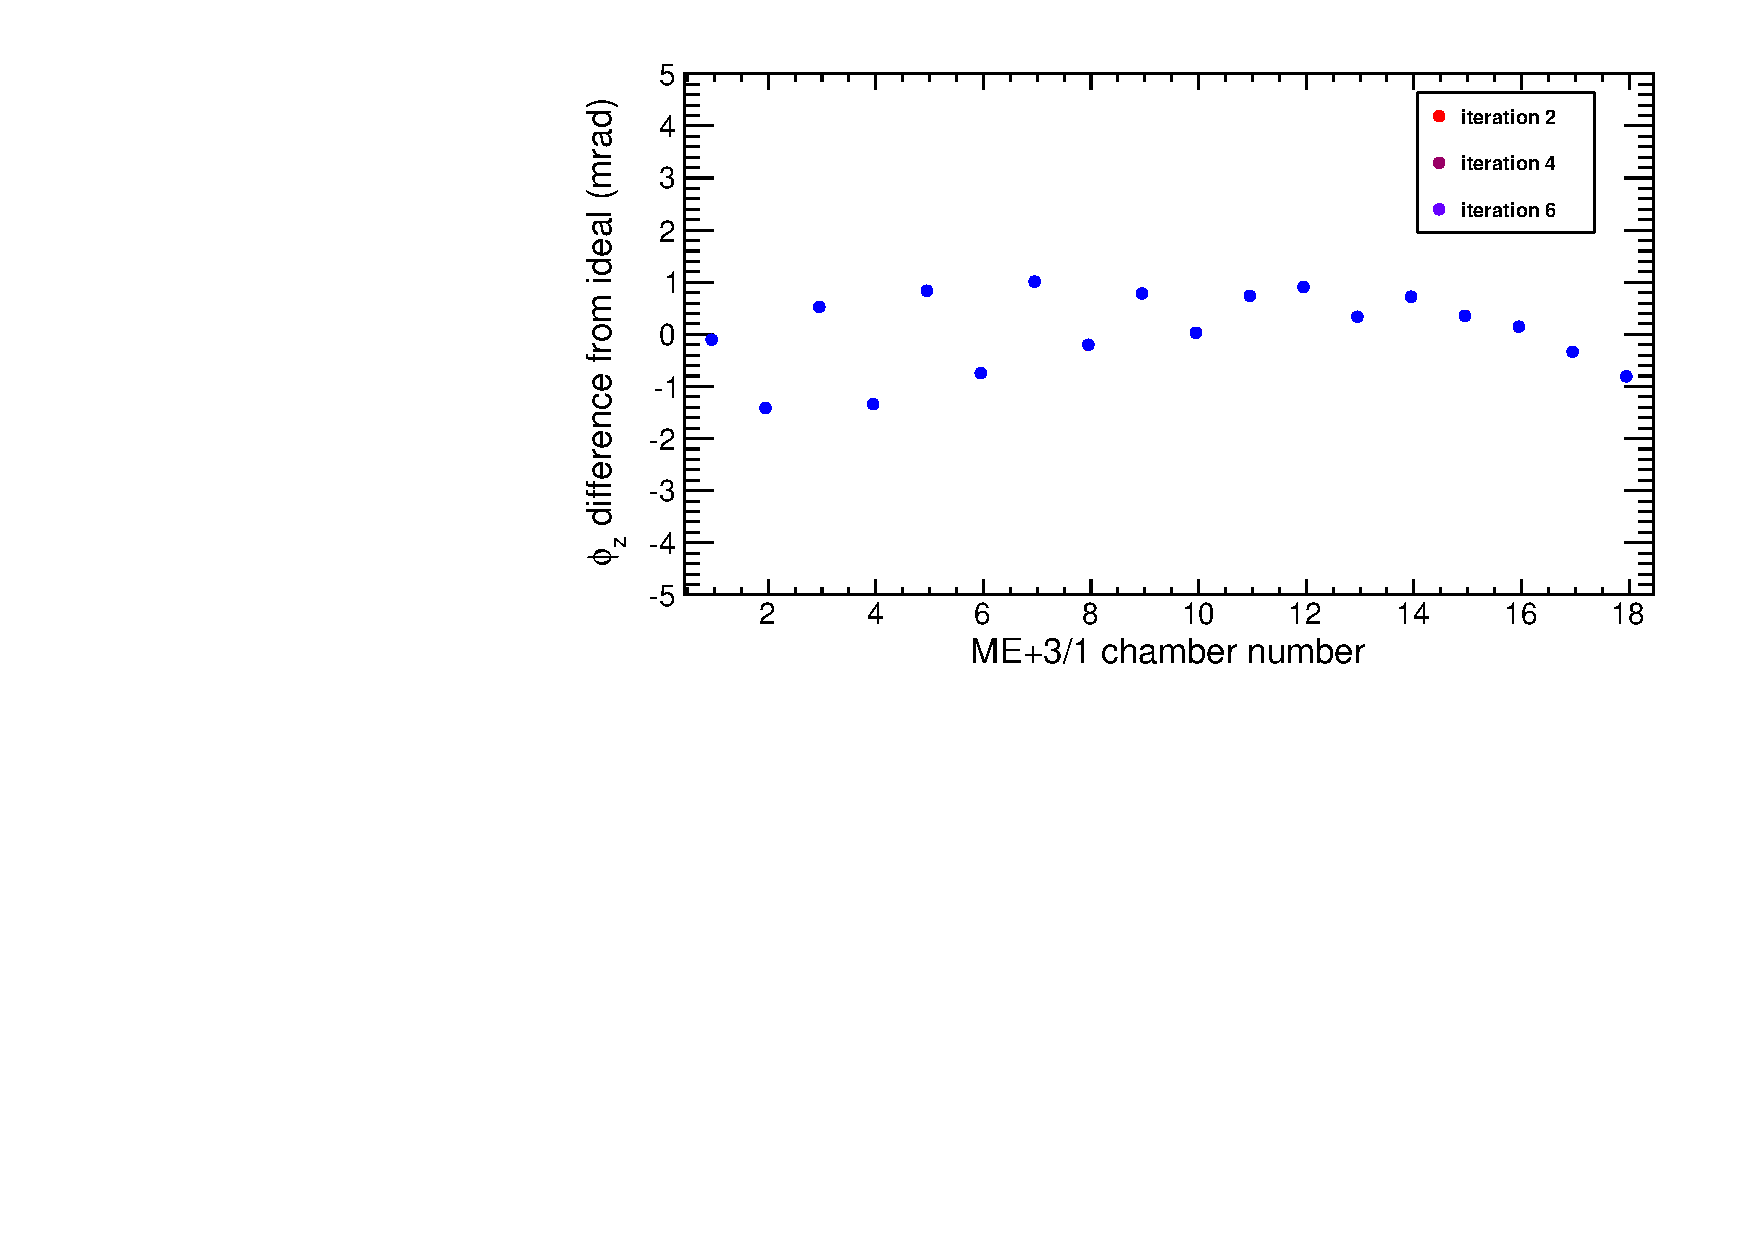
\includegraphics[width=0.6\linewidth]{newplots_convergence_mep31_phiz.pdf}

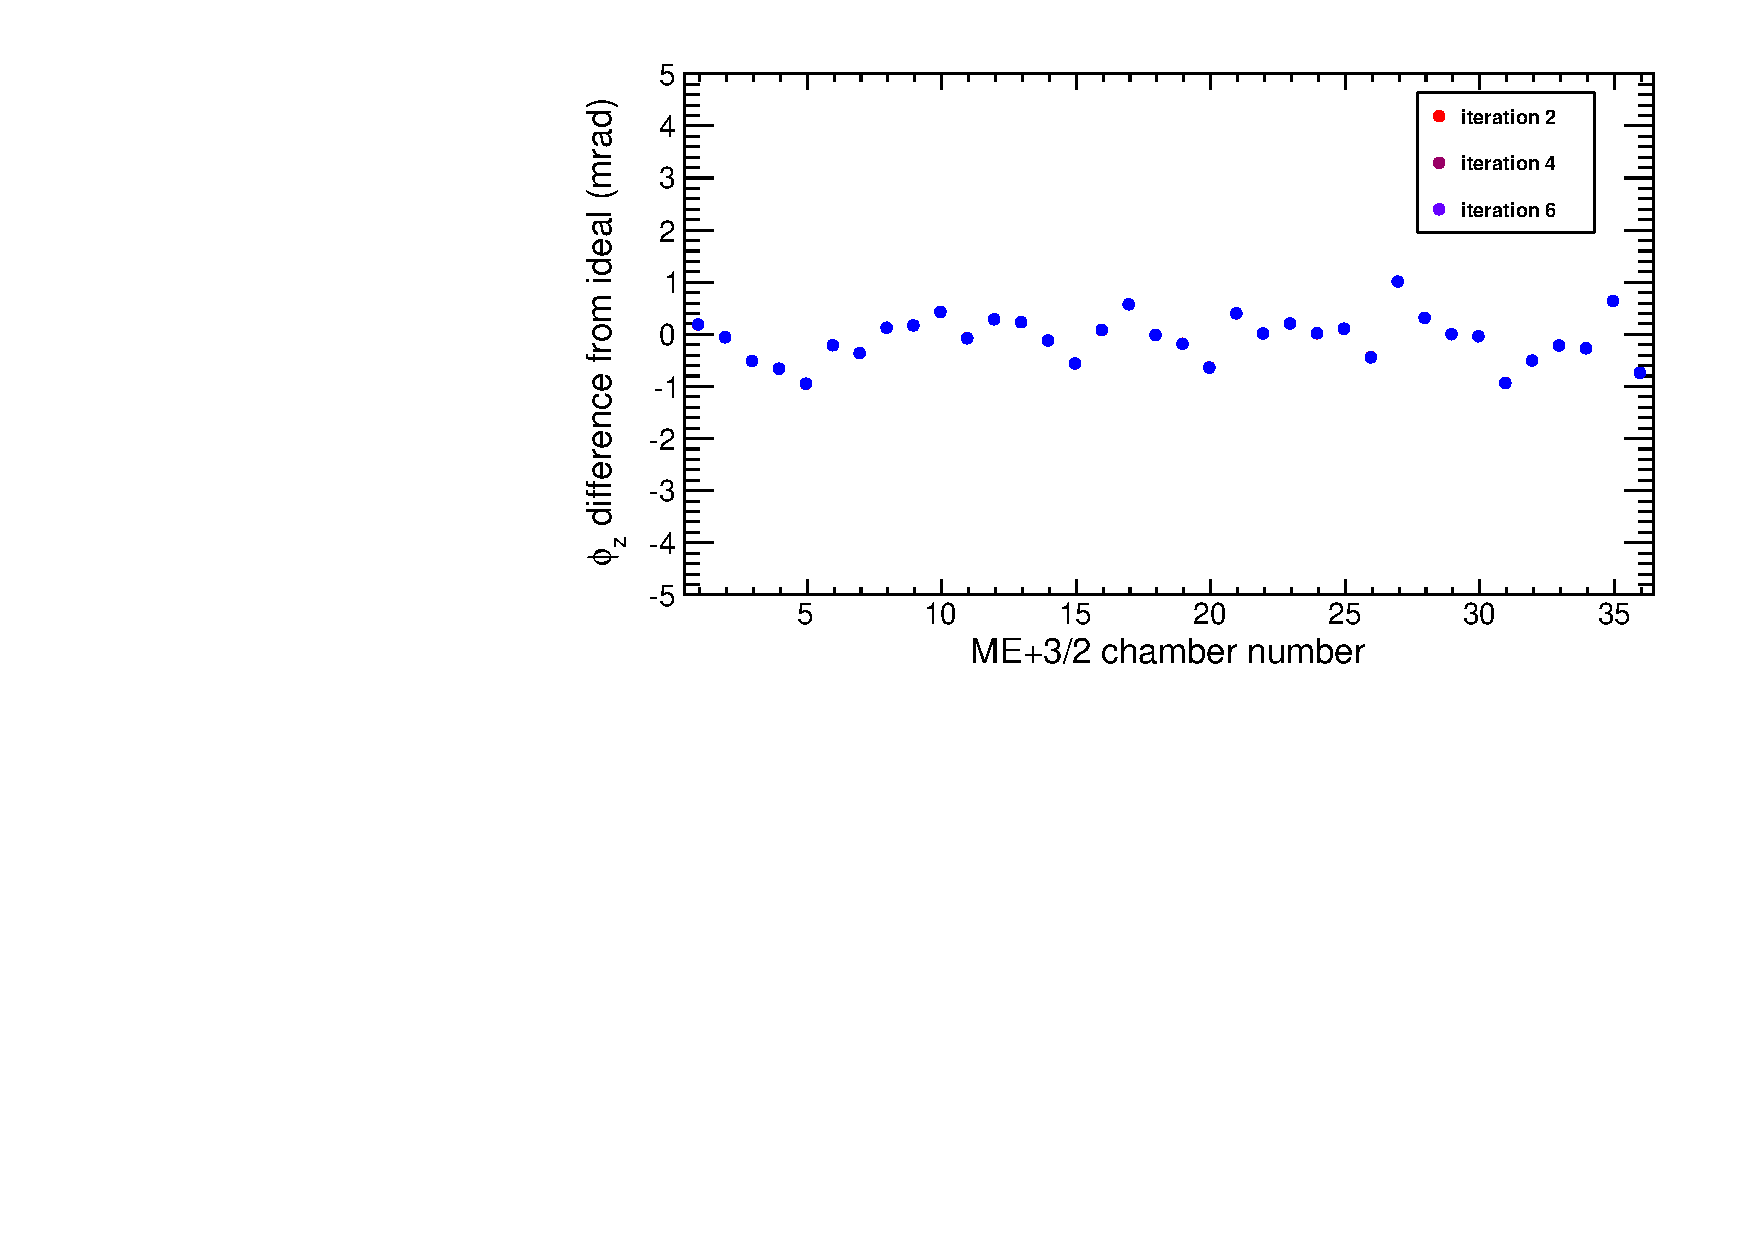
\includegraphics[width=0.6\linewidth]{newplots_convergence_mep32_phiz.pdf}}
\only<3>{Fit residuals in $\phi_z$ (not track residuals)

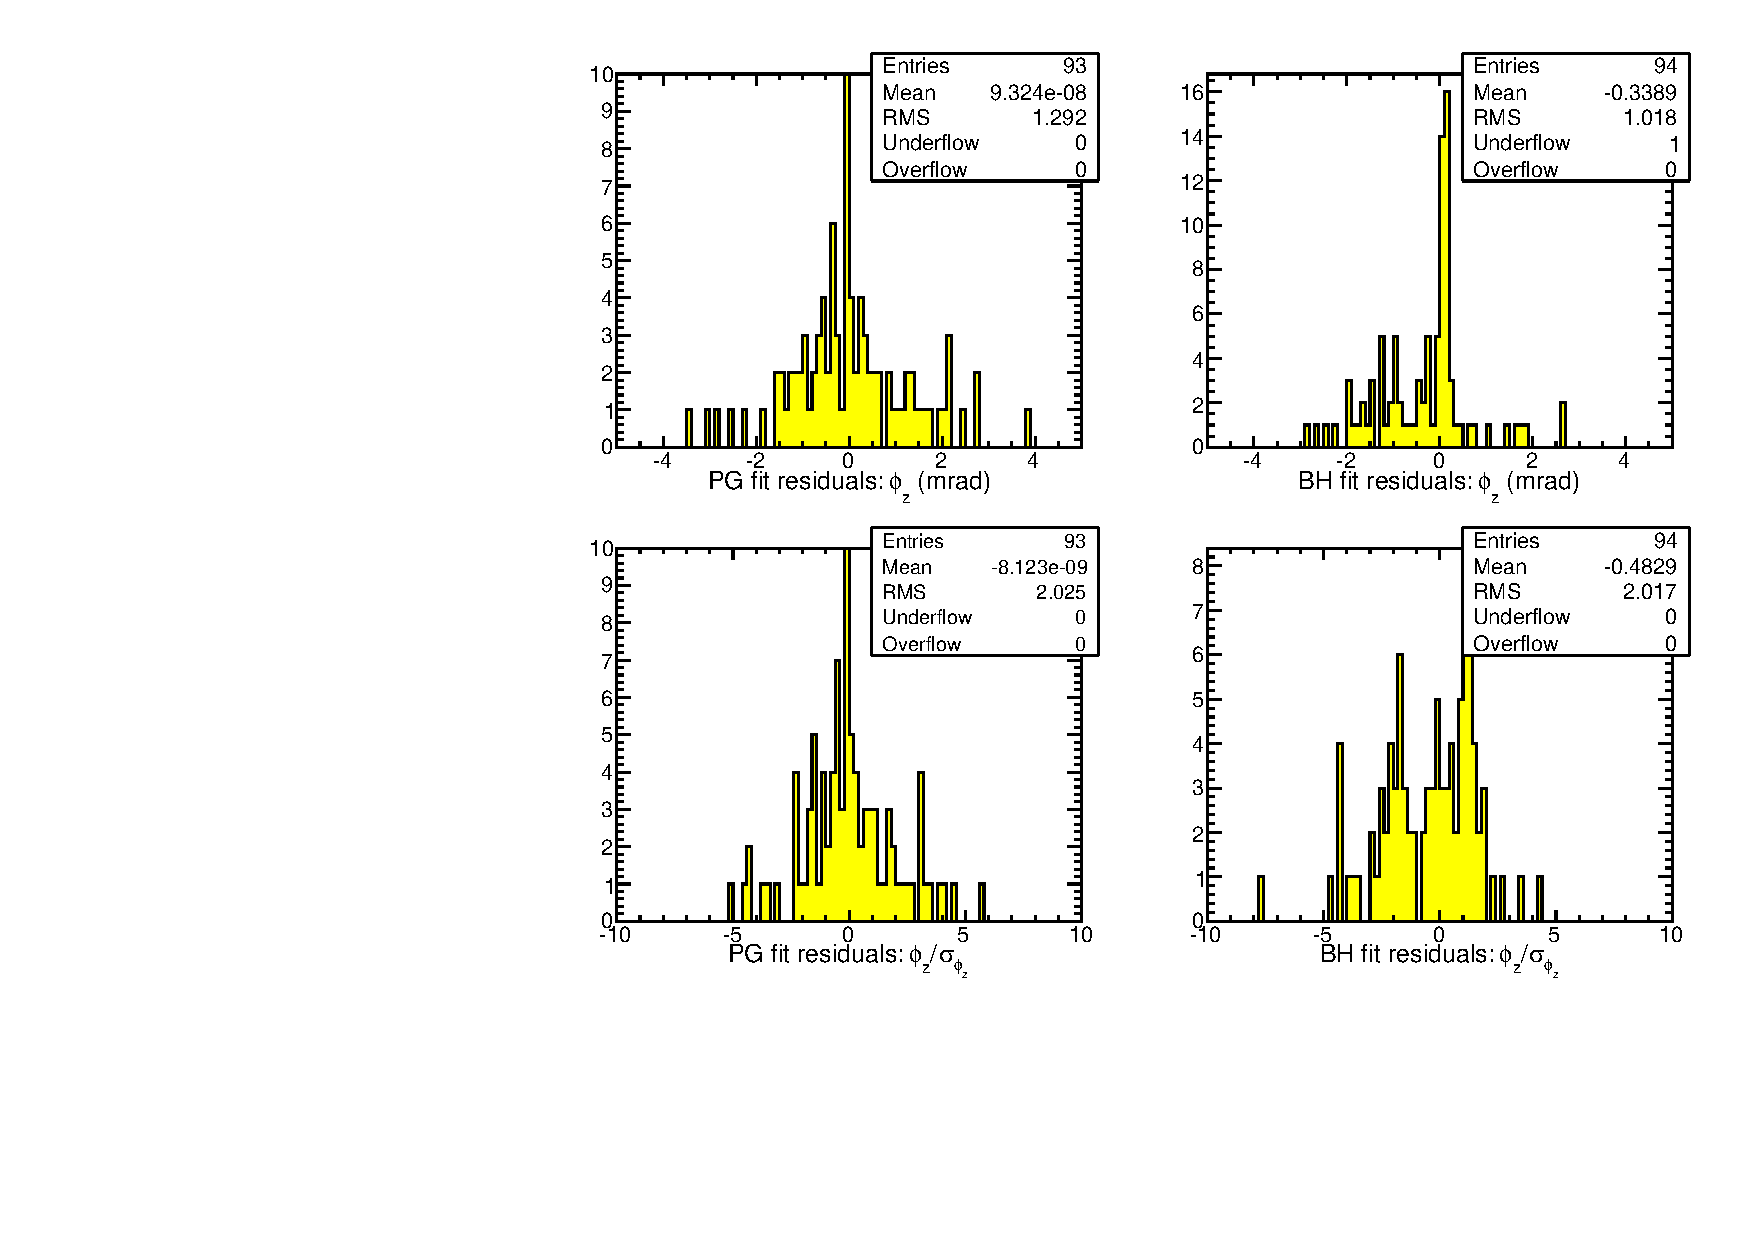
\includegraphics[width=0.9\linewidth]{newplots_fitresiduals_YEp2_phiz.pdf}}
\only<4>{Numbers in boxes are $\phi_z$ angle uncertainty in each mode in rad

First 2 are completely undetermined (uncertainty is meaningless)

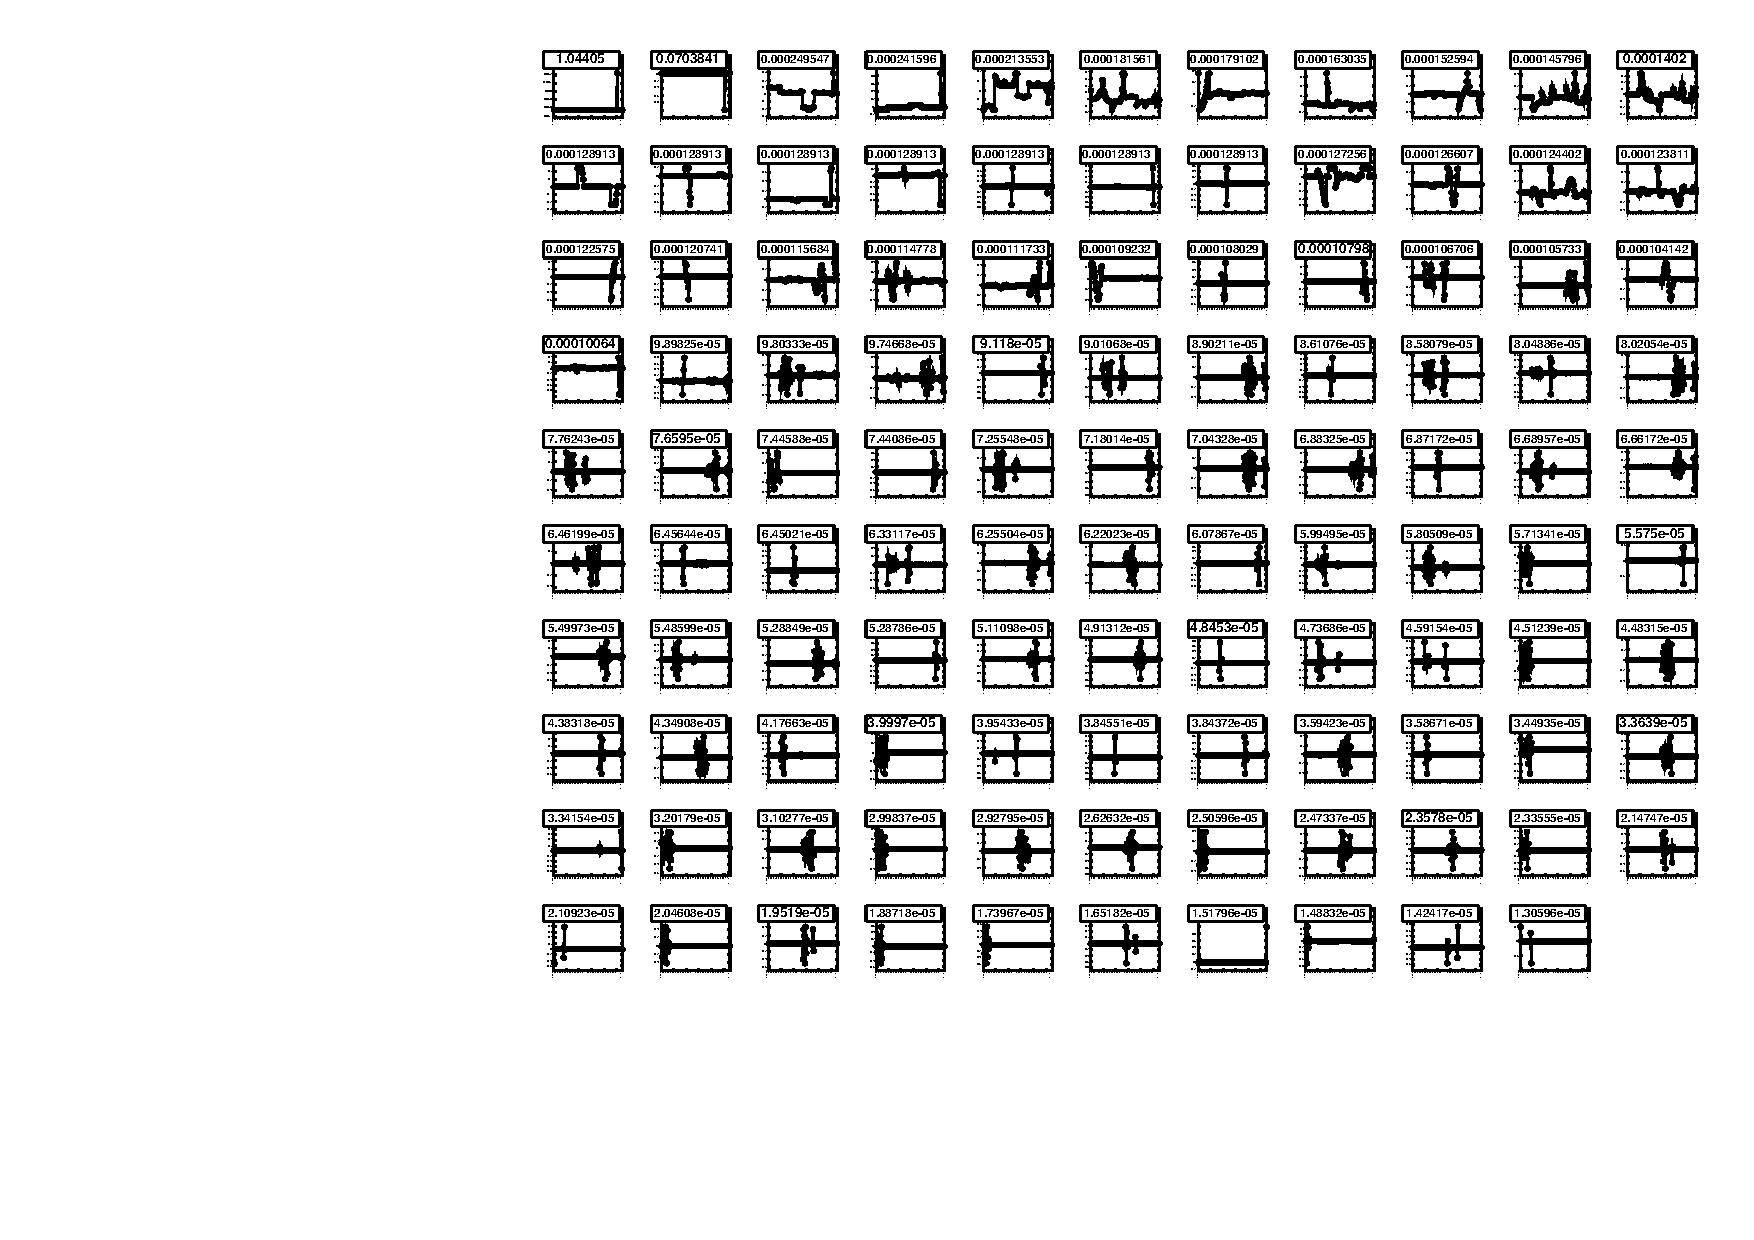
\includegraphics[width=0.9\linewidth]{newplots_errors_YEp2_phiz.pdf}}
\end{frame}

\begin{frame}
\frametitle{YE$-$2 $r\phi$}

\only<1>{Convergence in $r\phi$ positions

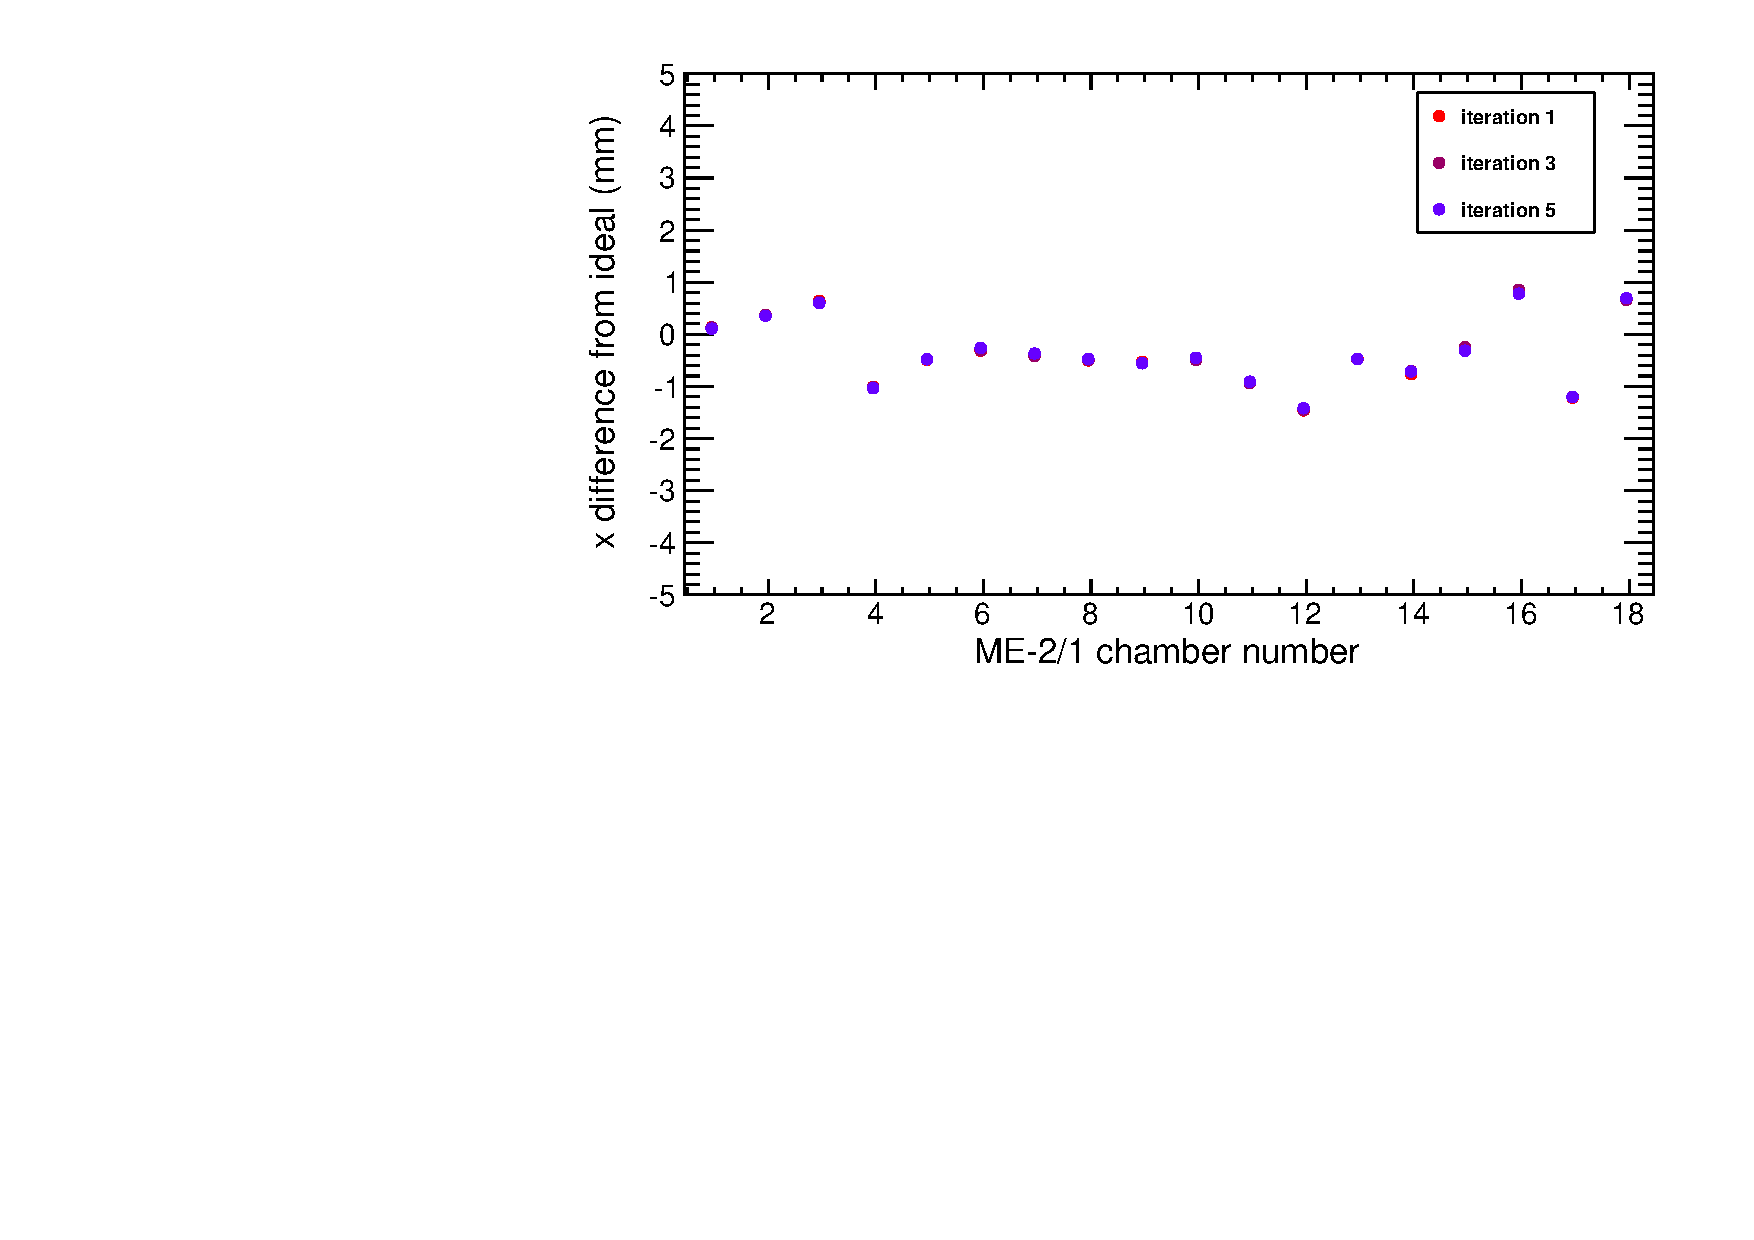
\includegraphics[width=0.6\linewidth]{newplots_convergence_mem21_x.pdf}

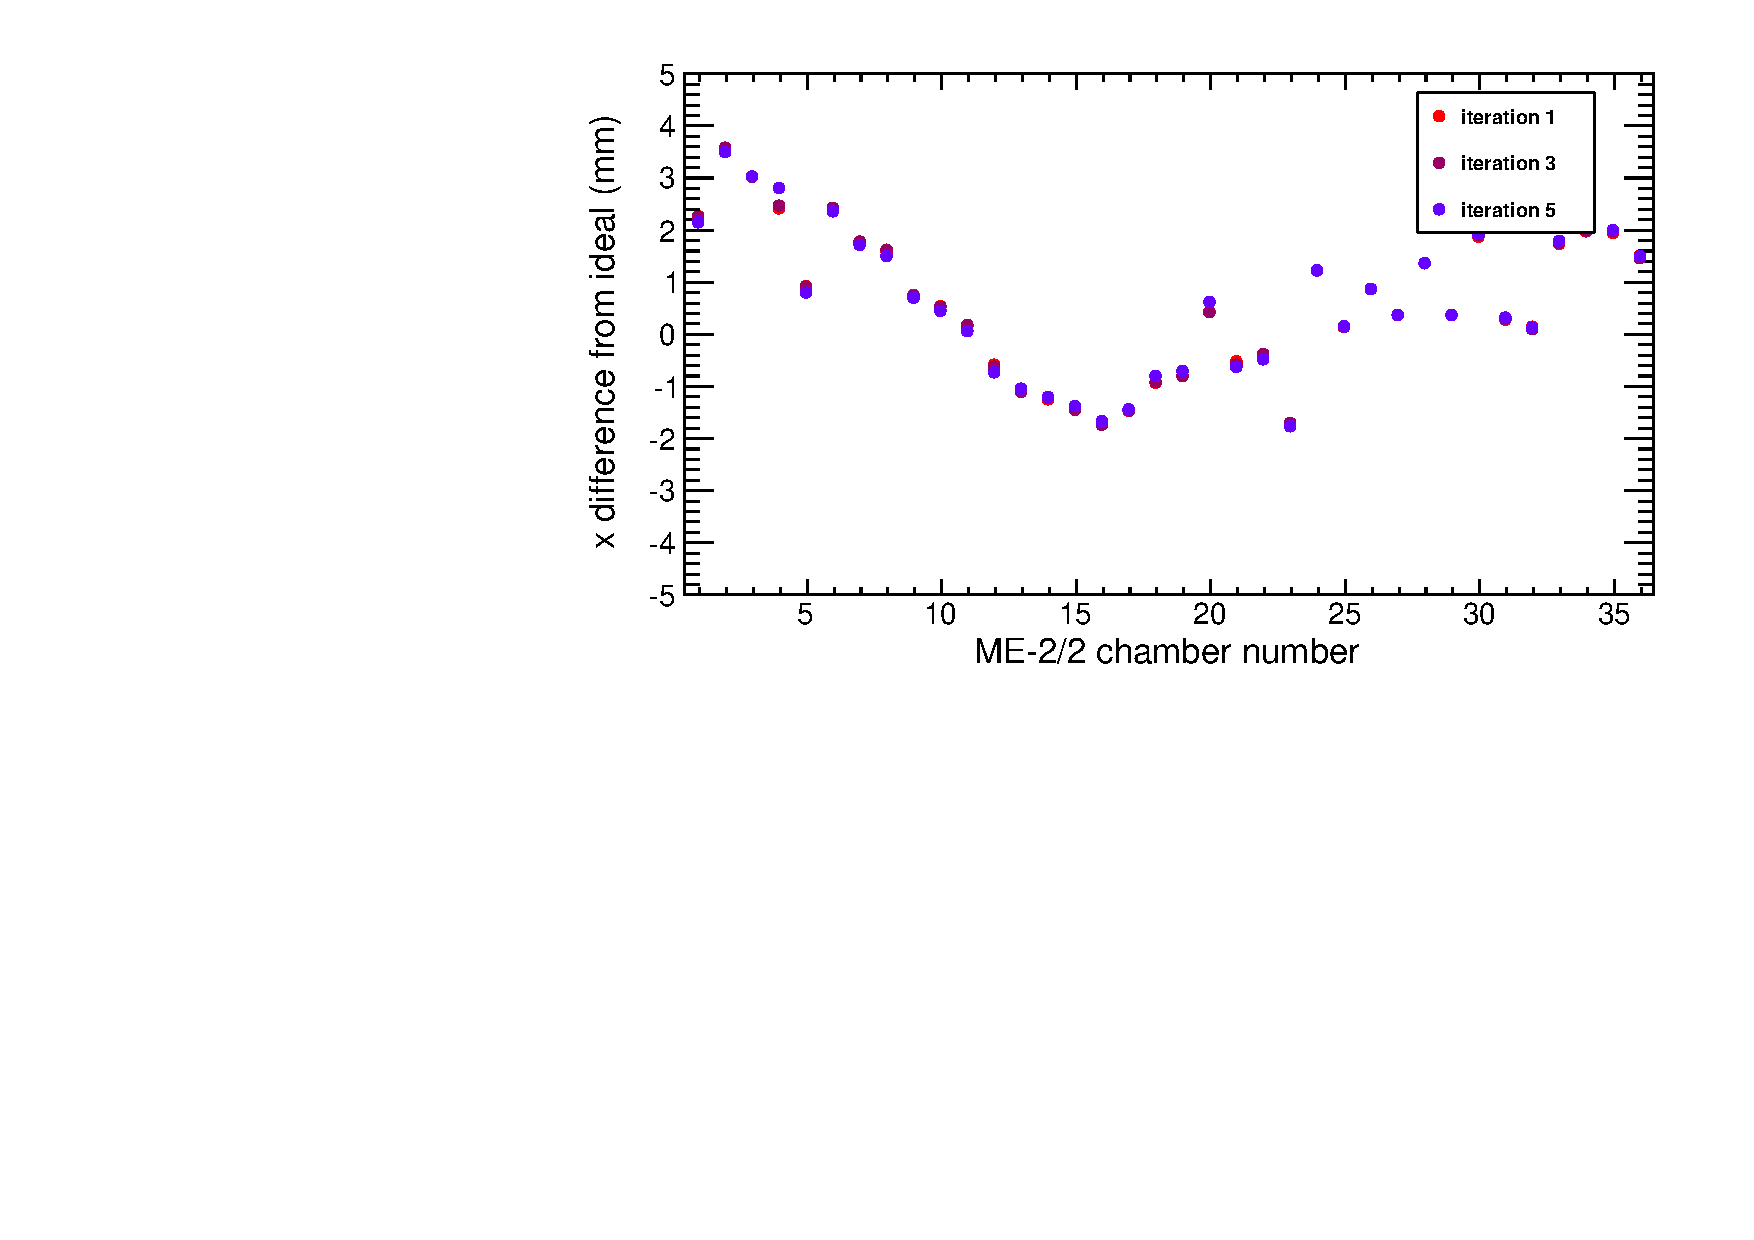
\includegraphics[width=0.6\linewidth]{newplots_convergence_mem22_x.pdf}}
\only<2>{Convergence in $r\phi$ positions

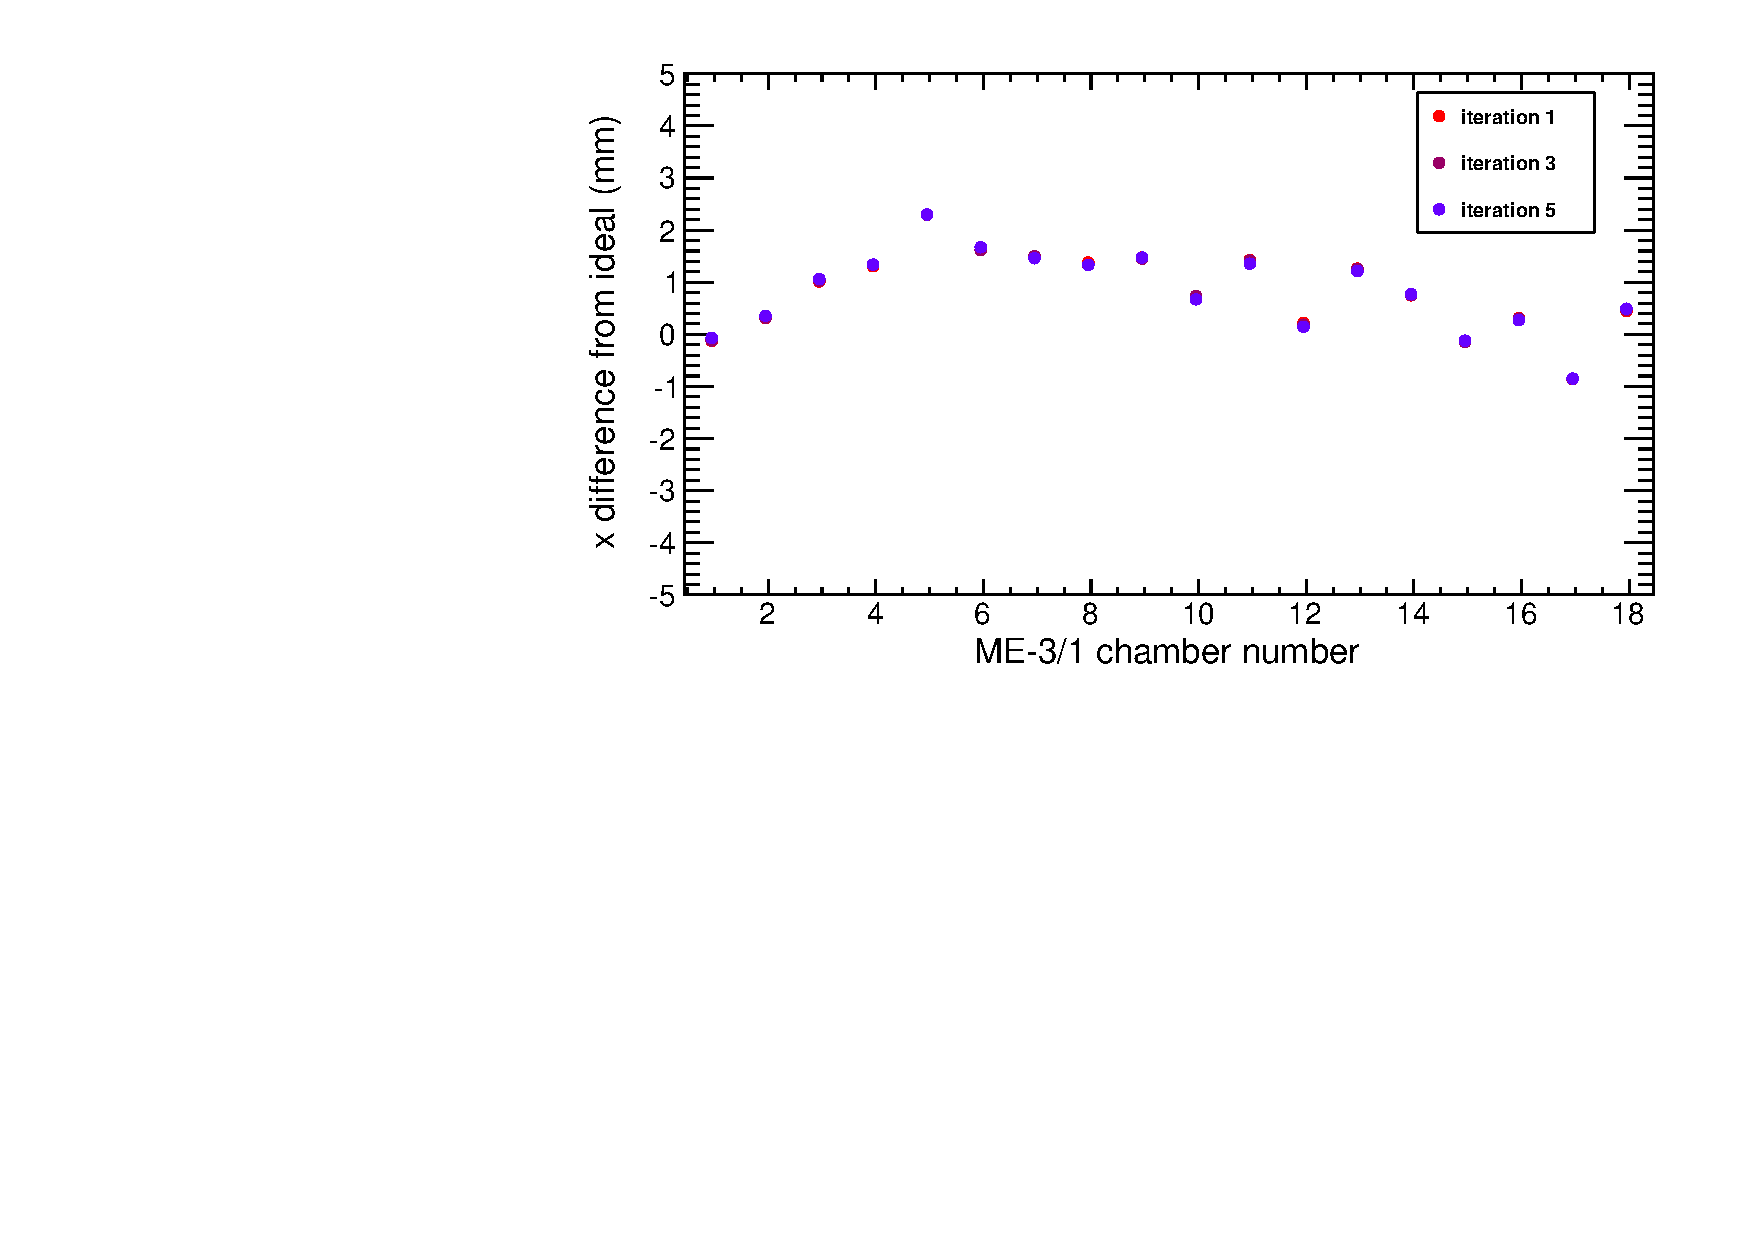
\includegraphics[width=0.6\linewidth]{newplots_convergence_mem31_x.pdf}

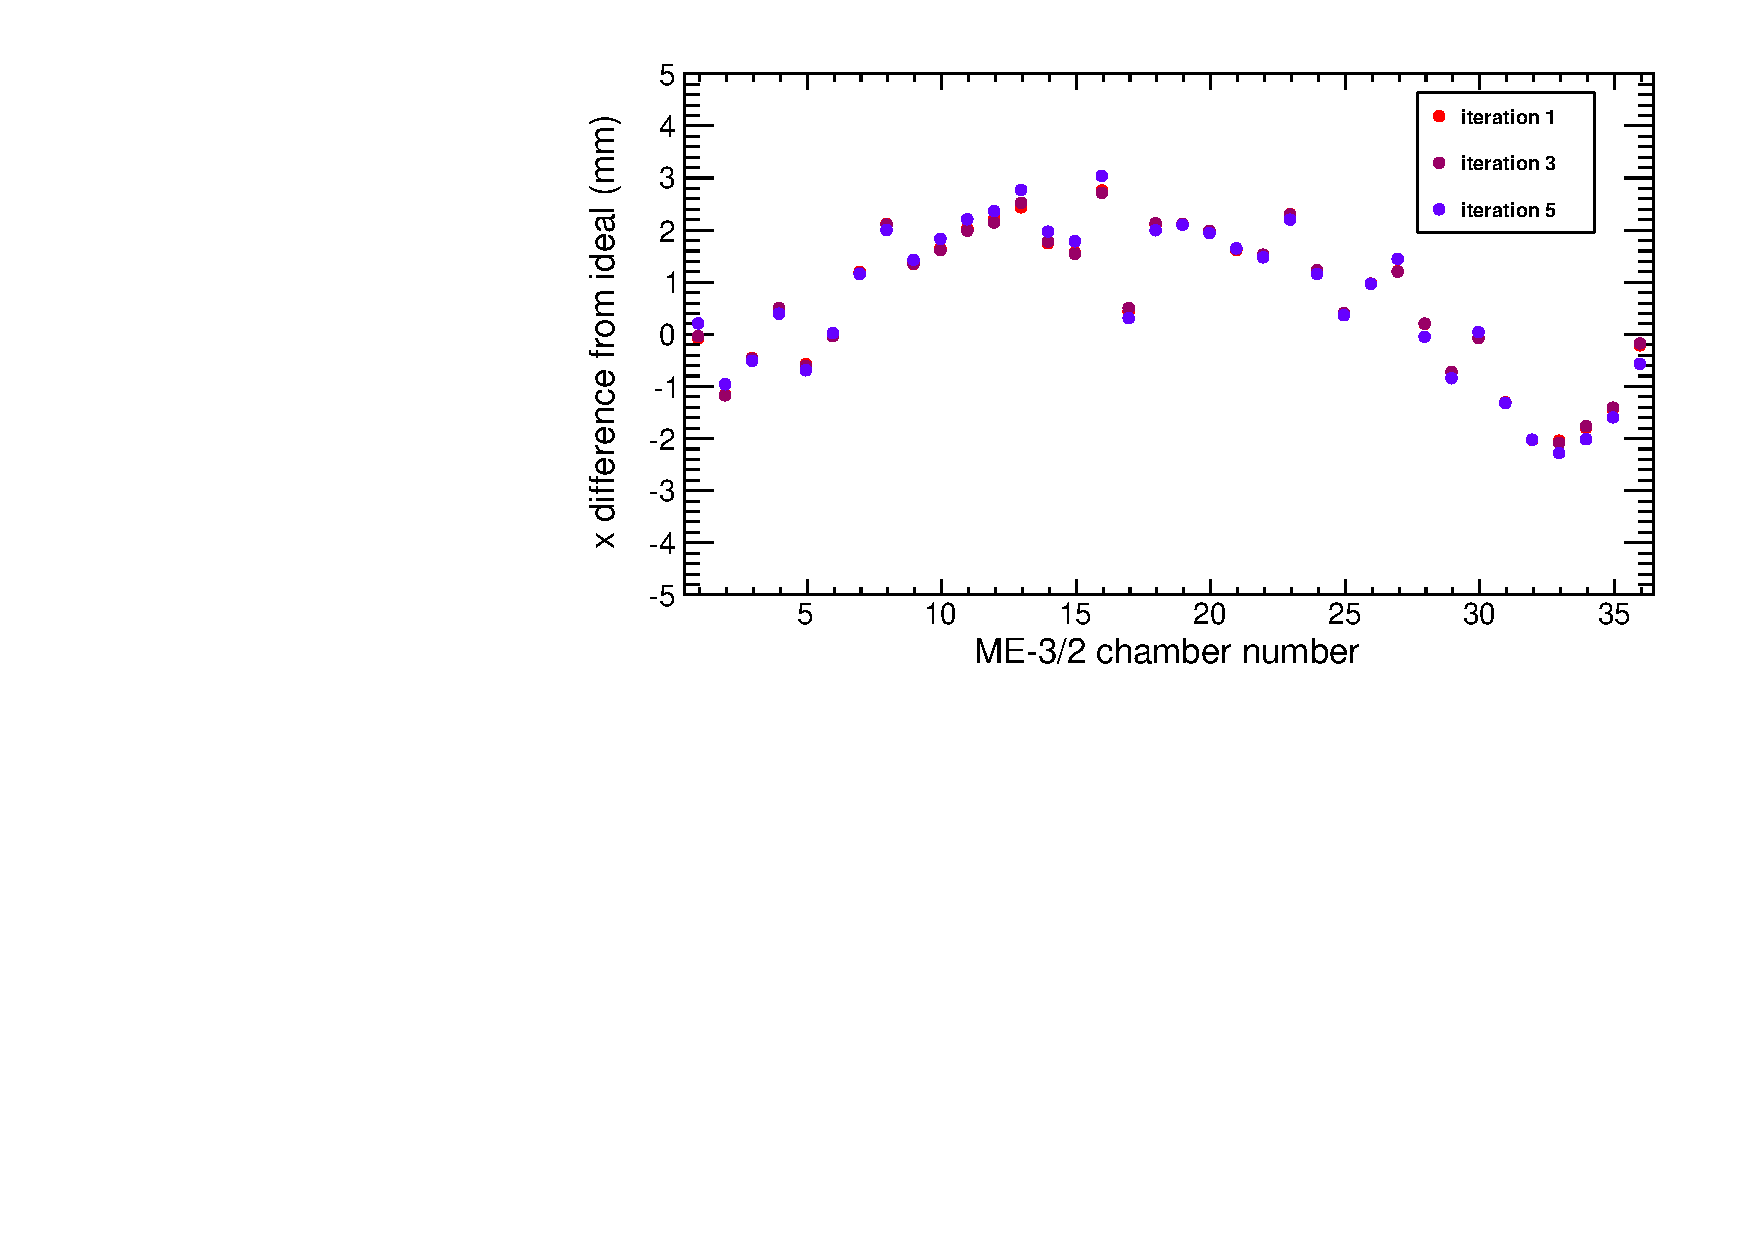
\includegraphics[width=0.6\linewidth]{newplots_convergence_mem32_x.pdf}}
\only<3>{Fit residuals in $r\phi$ (not track residuals)

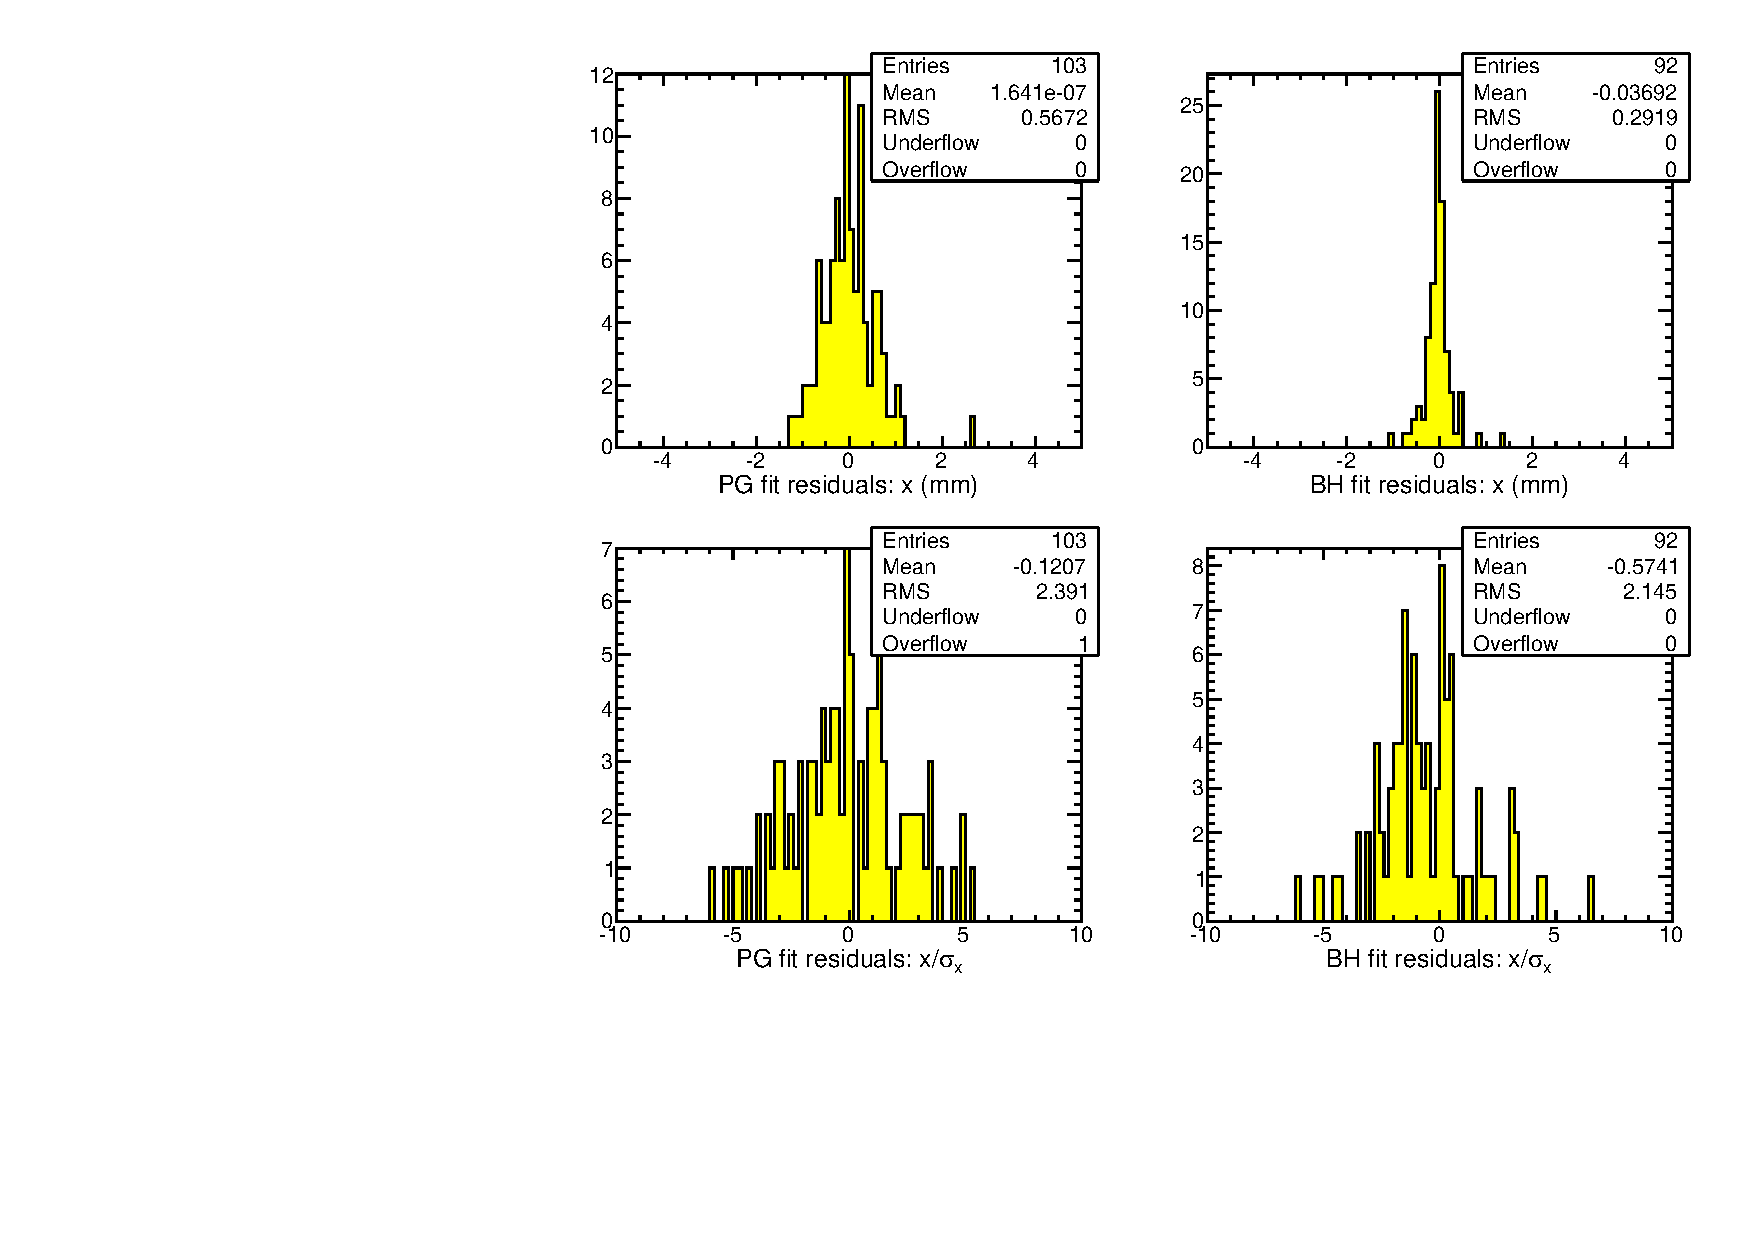
\includegraphics[width=0.9\linewidth]{newplots_fitresiduals_YEm2_x.pdf}}
\only<4>{Numbers in boxes are $\phi$ position uncertainty in each mode in rad

First 2 are completely undetermined (uncertainty is meaningless)

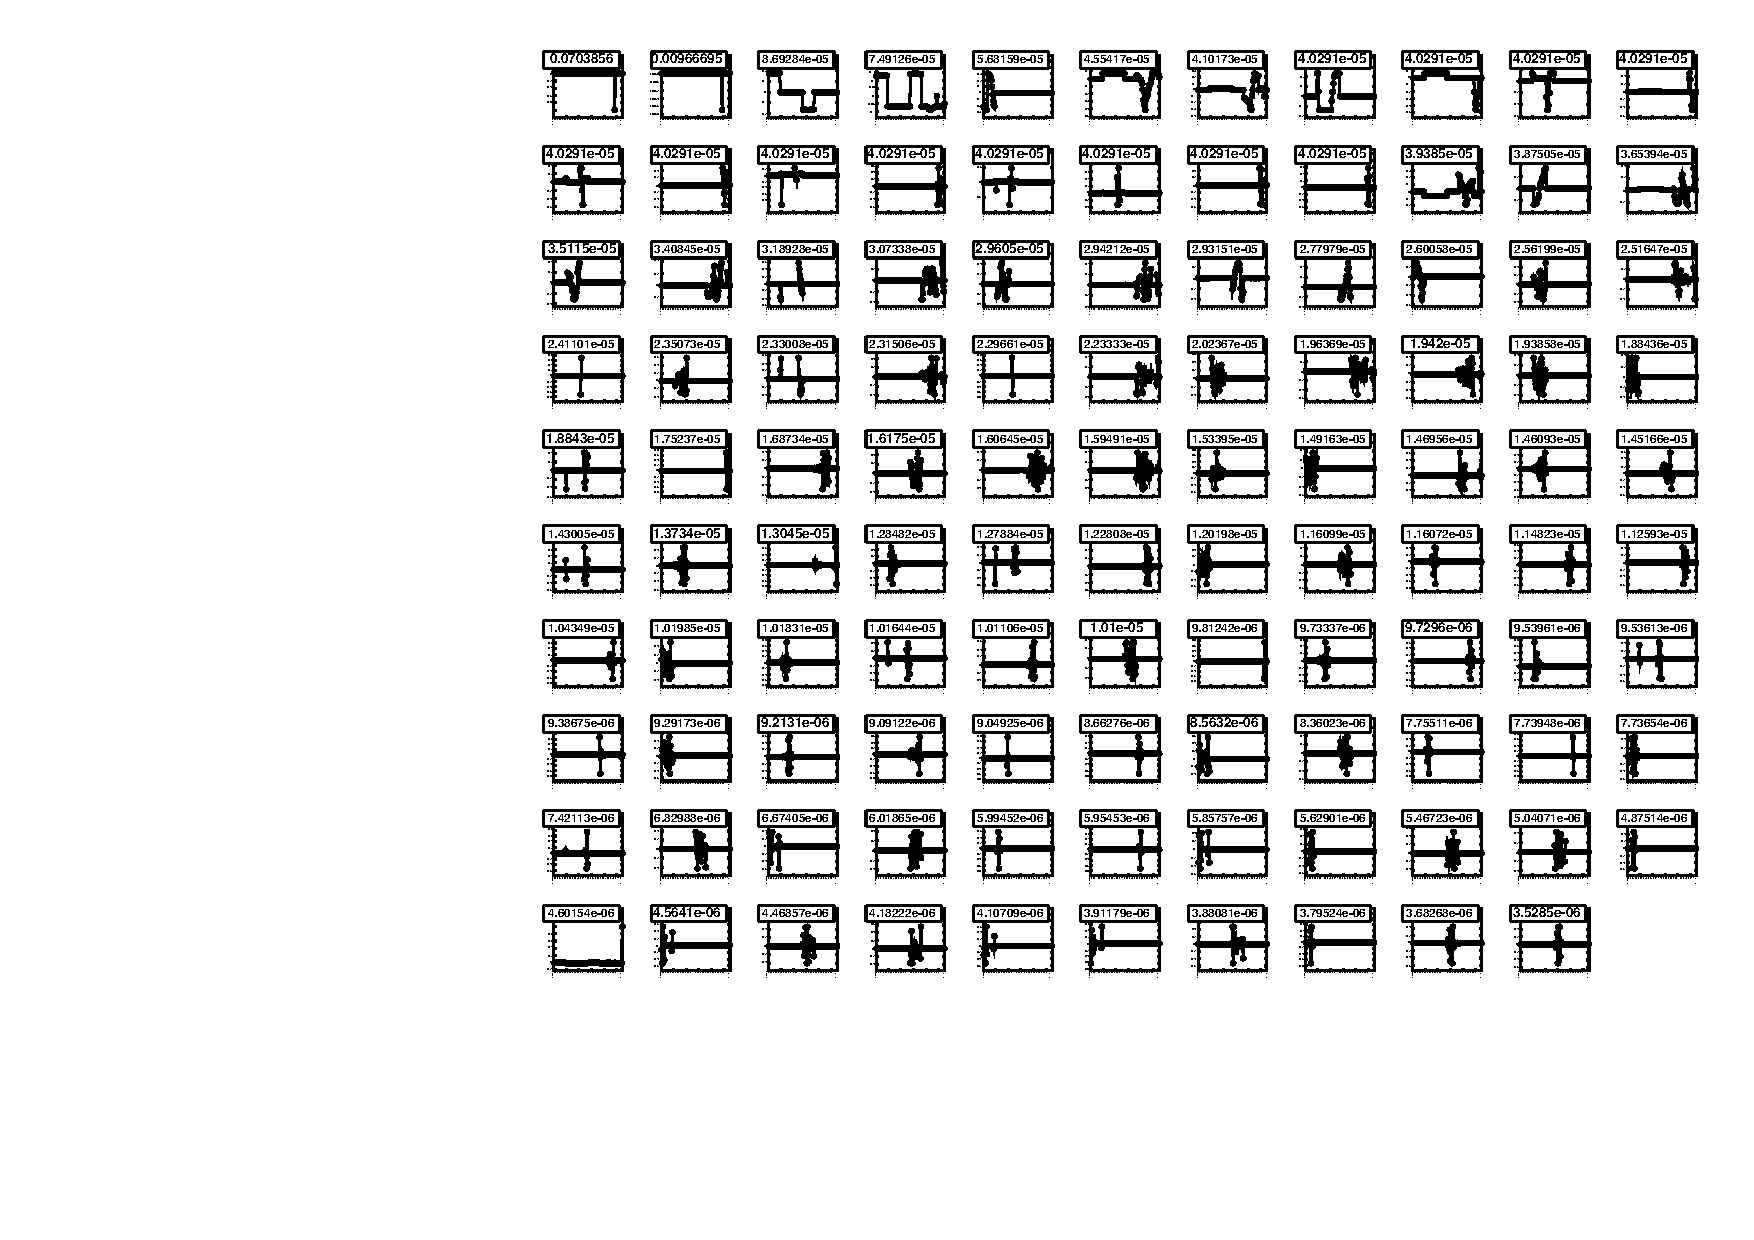
\includegraphics[width=0.9\linewidth]{newplots_errors_YEm2_x.pdf}}
\end{frame}

\begin{frame}
\frametitle{YE$-$2 $\phi_z$}

\only<1>{Convergence in $\phi_z$ positions

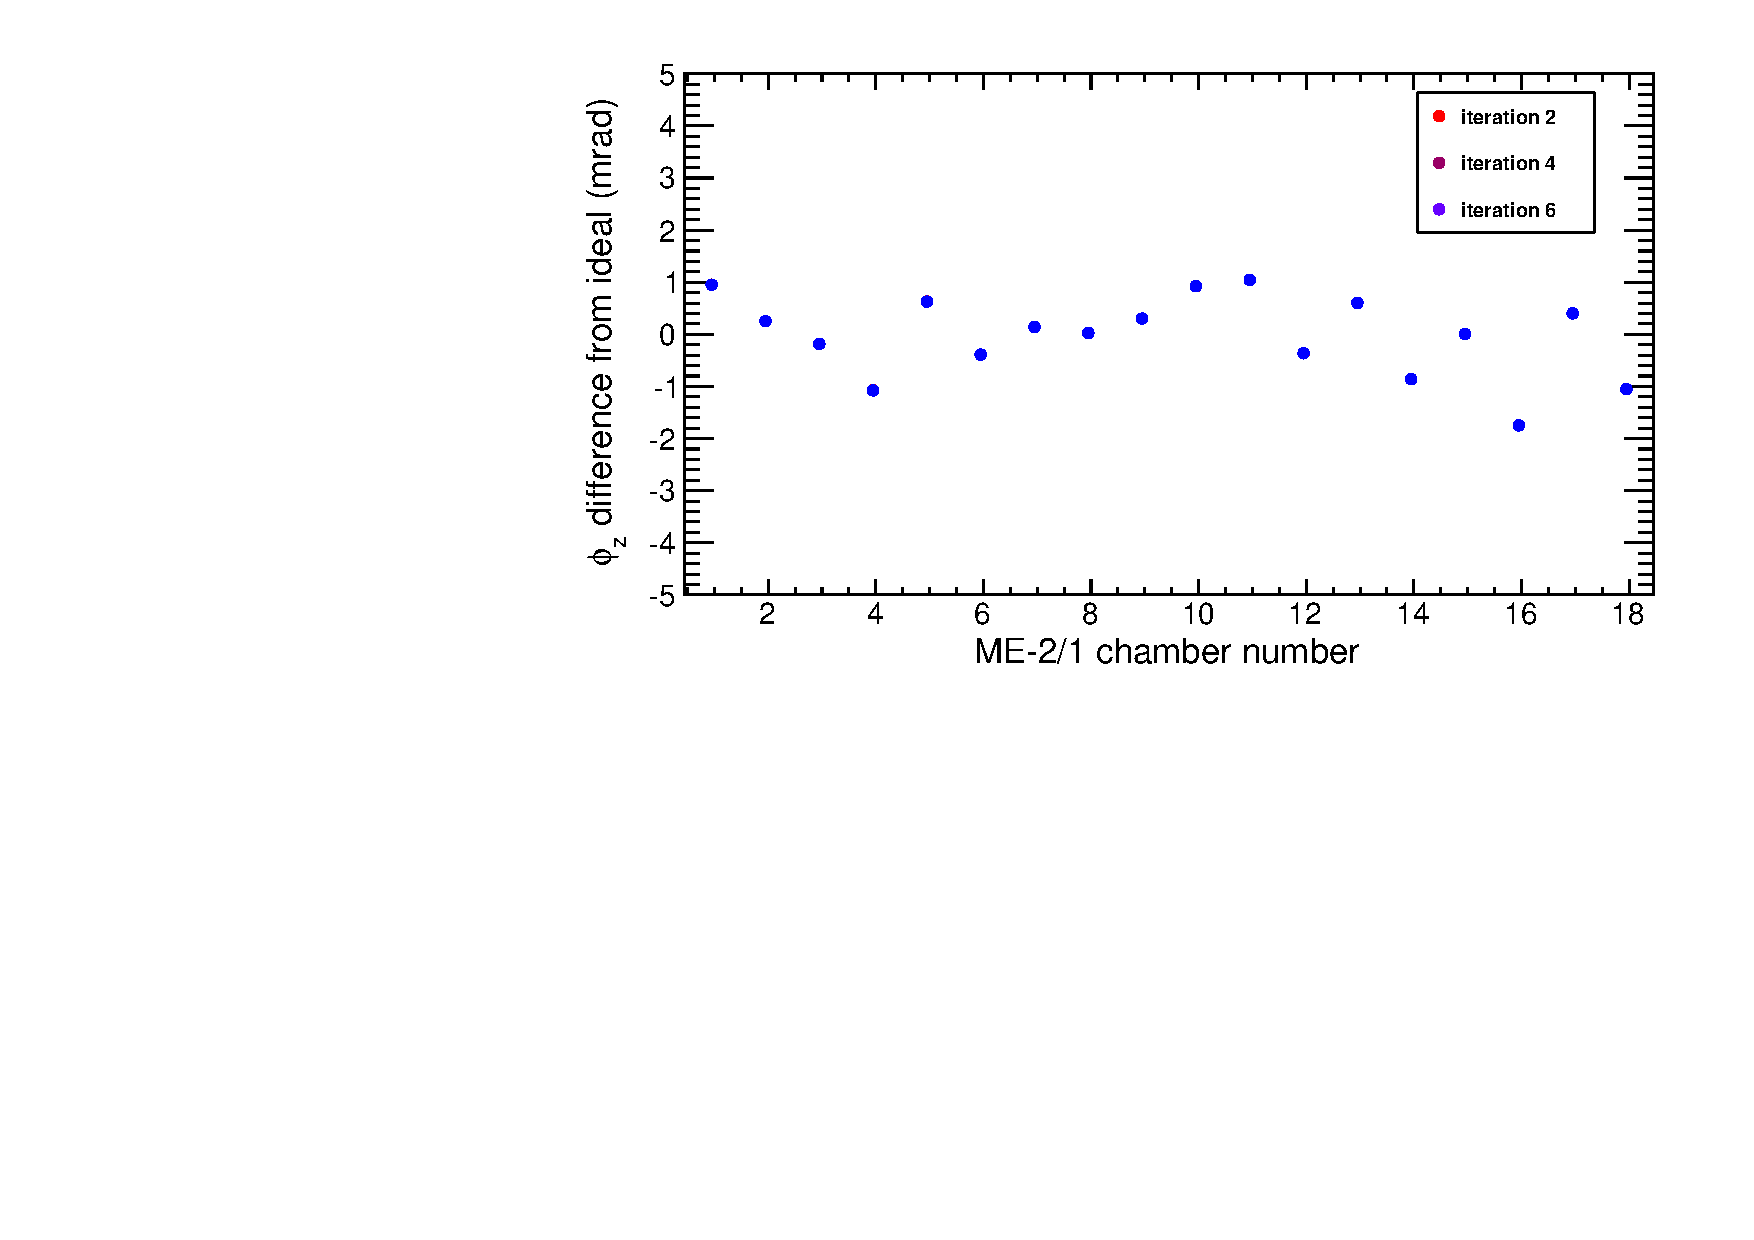
\includegraphics[width=0.6\linewidth]{newplots_convergence_mem21_phiz.pdf}

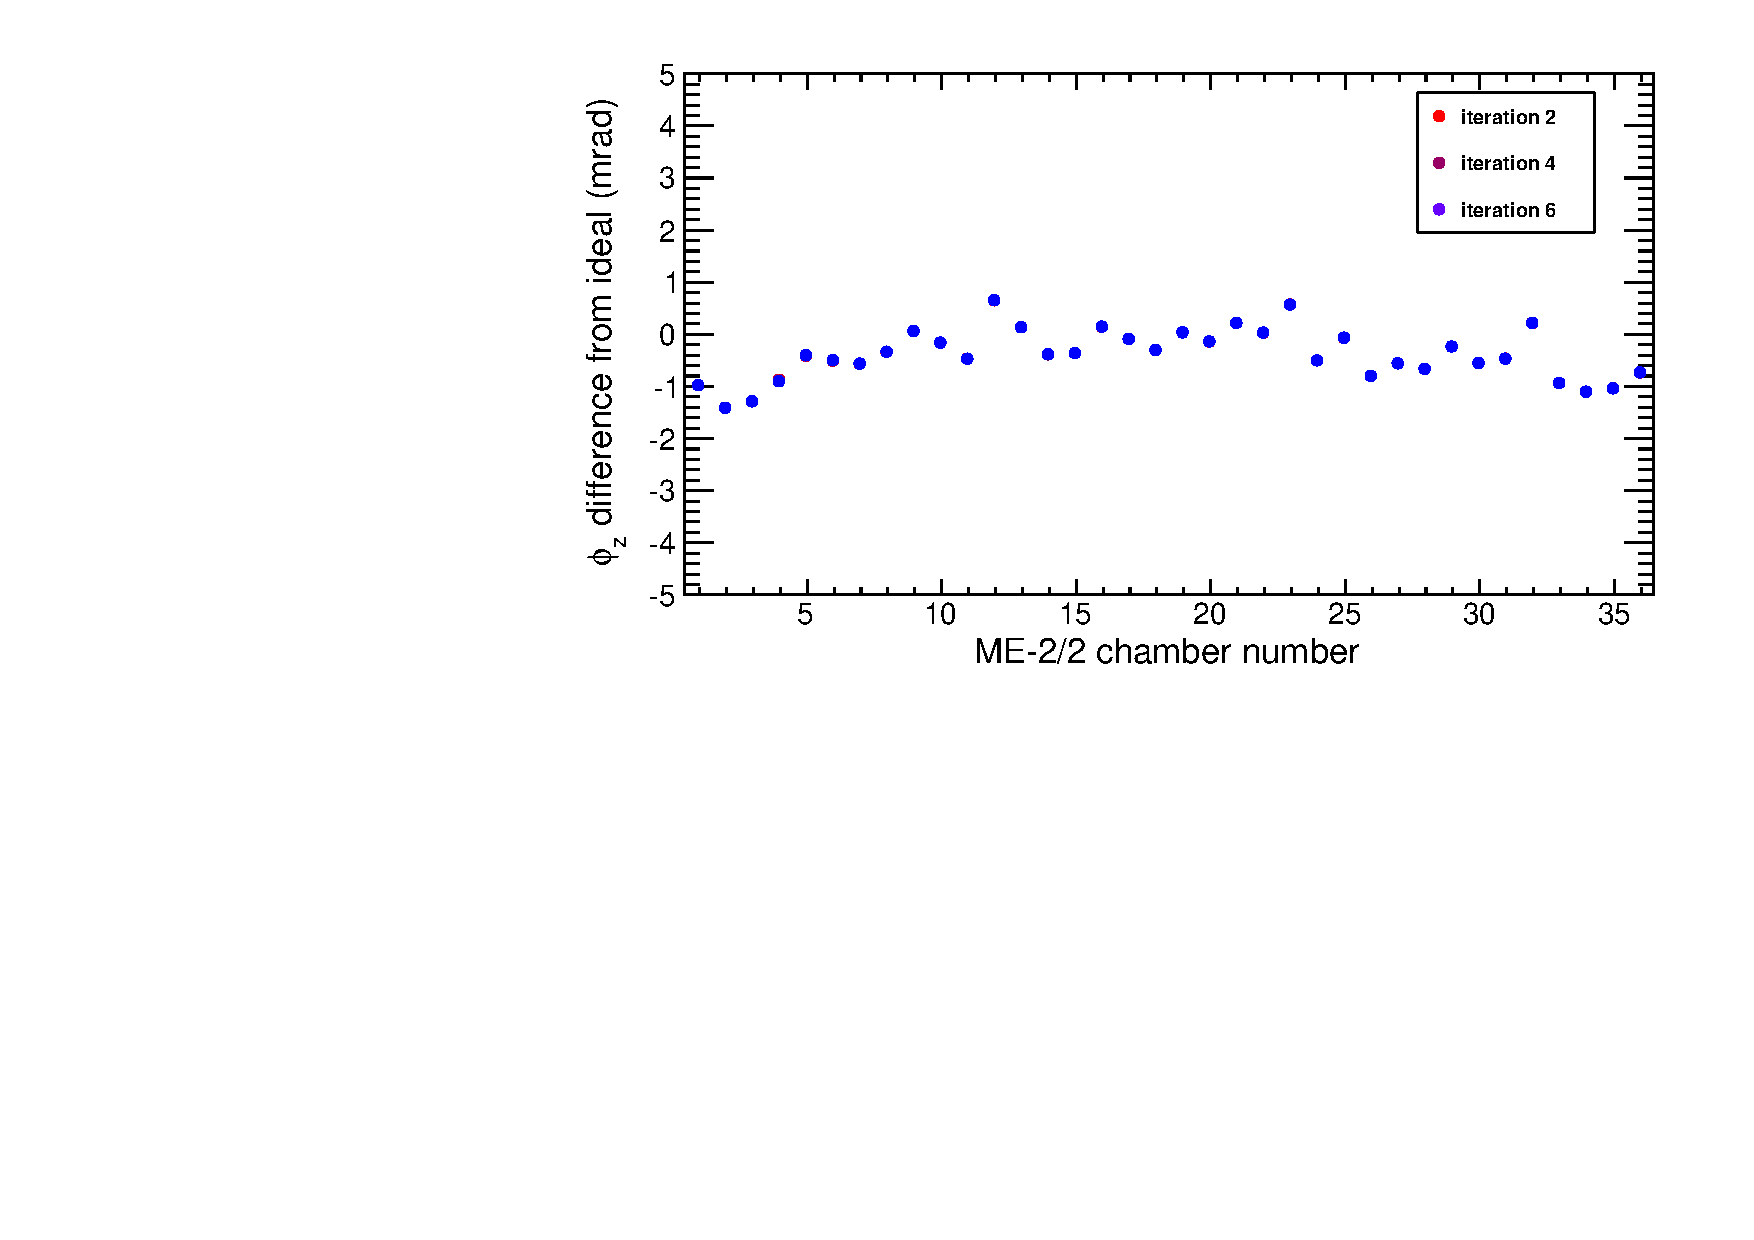
\includegraphics[width=0.6\linewidth]{newplots_convergence_mem22_phiz.pdf}}
\only<2>{Convergence in $\phi_z$ positions

\includegraphics[width=0.6\linewidth]{newplots_convergence_mem31_phiz.pdf}

\includegraphics[width=0.6\linewidth]{newplots_convergence_mem32_phiz.pdf}}
\only<3>{Fit residuals in $\phi_z$ (not track residuals)

\includegraphics[width=0.9\linewidth]{newplots_fitresiduals_YEm2_phiz.pdf}}
\only<4>{Numbers in boxes are $\phi_z$ angle uncertainty in each mode in rad

First 2 are completely undetermined (uncertainty is meaningless)

\includegraphics[width=0.9\linewidth]{newplots_errors_YEm2_phiz.pdf}}
\end{frame}

\begin{frame}
\frametitle{ME$+$4/1 $r\phi$}

\only<1>{Convergence in $r\phi$ positions

\includegraphics[width=\linewidth]{newplots_convergence_mep41_x.pdf}}
\only<2>{Fit residuals in $r\phi$ (not track residuals)

\includegraphics[width=0.9\linewidth]{newplots_fitresiduals_MEp4_1_x.pdf}}
\only<3>{Numbers in boxes are $\phi$ position uncertainty in each mode in rad

First 1 is completely undetermined (uncertainty is meaningless)

\includegraphics[width=0.9\linewidth]{newplots_errors_MEp4_1_x.pdf}}
\end{frame}

\begin{frame}
\frametitle{ME$+$4/1 $\phi_z$}

\only<1>{Convergence in $\phi_z$ angles

\includegraphics[width=\linewidth]{newplots_convergence_mep41_phiz.pdf}}
\only<2>{Fit residuals in $\phi_z$ (not track residuals)

\includegraphics[width=0.9\linewidth]{newplots_fitresiduals_MEp4_1_phiz.pdf}}
\only<3>{Numbers in boxes are $\phi_z$ angle uncertainty in each mode in rad

First 1 is completely undetermined (uncertainty is meaningless)

\includegraphics[width=0.9\linewidth]{newplots_errors_MEp4_1_phiz.pdf}}
\end{frame}

\begin{frame}
\frametitle{ME$-$4/1 $r\phi$}

\only<1>{Convergence in $r\phi$ positions

\includegraphics[width=\linewidth]{newplots_convergence_mem41_x.pdf}}
\only<2>{Fit residuals in $r\phi$ (not track residuals)

\includegraphics[width=0.9\linewidth]{newplots_fitresiduals_MEm4_1_x.pdf}}
\only<3>{Numbers in boxes are $\phi$ position uncertainty in each mode in rad

First 1 is completely undetermined (uncertainty is meaningless)

\includegraphics[width=0.9\linewidth]{newplots_errors_MEm4_1_x.pdf}}
\end{frame}

\begin{frame}
\frametitle{ME$-$4/1 $\phi_z$}

\only<1>{Convergence in $\phi_z$ angles

\includegraphics[width=\linewidth]{newplots_convergence_mem41_phiz.pdf}}
\only<2>{Fit residuals in $\phi_z$ (not track residuals)

\includegraphics[width=0.9\linewidth]{newplots_fitresiduals_MEm4_1_phiz.pdf}}
\only<3>{Numbers in boxes are $\phi_z$ angle uncertainty in each mode in rad

First 1 is completely undetermined (uncertainty is meaningless)

\includegraphics[width=0.9\linewidth]{newplots_errors_MEm4_1_phiz.pdf}}
\end{frame}

\begin{frame}
\frametitle{ME$+$4/2 $r\phi$}

\only<1>{Convergence in $r\phi$ positions

\includegraphics[width=\linewidth]{newplots_convergence_mep42_x.pdf}}
\only<2>{Fit residuals in $r\phi$ (not track residuals): no PG, perfect BH fit

\includegraphics[width=0.9\linewidth]{newplots_fitresiduals_MEp4_2_x.pdf}}
\only<3>{Numbers in boxes are $\phi$ position uncertainty in each mode in rad

First 1 is completely undetermined (uncertainty is meaningless)

\includegraphics[width=0.9\linewidth]{newplots_errors_MEp4_2_x.pdf}}
\end{frame}

\begin{frame}
\frametitle{ME$+$4/2 $\phi_z$}

\only<1>{Convergence in $\phi_z$ angles

\includegraphics[width=\linewidth]{newplots_convergence_mep42_phiz.pdf}}
\only<2>{Fit residuals in $\phi_z$ (not track residuals): no PG, perfect BH fit

\includegraphics[width=0.9\linewidth]{newplots_fitresiduals_MEp4_2_phiz.pdf}}
\only<3>{Numbers in boxes are $\phi_z$ angle uncertainty in each mode in rad

First 1 is completely undetermined (uncertainty is meaningless)

\includegraphics[width=0.9\linewidth]{newplots_errors_MEp4_2_phiz.pdf}}
\end{frame}

\begin{frame}
\frametitle{globalMuon ring alignment}

\begin{itemize}
\item Using 2010 cosmics, align large structures to tracker
\item This is a test without the latest tracker and GlobalPositionRcd
\item Inner ring alignment is not feasible with this dataset, so
  that's why we will combine disk statistics
\end{itemize}

\only<1>{\includegraphics[width=0.5\linewidth]{map_CSCvsphi_x_outer.png} \includegraphics[width=0.5\linewidth]{map_CSCvsphi_x_inner.png}}
\only<2>{\includegraphics[width=0.5\linewidth]{map_CSCvsphi_x_outerafter.png} \includegraphics[width=0.5\linewidth]{map_CSCvsphi_x_innerafter.png}}
\end{frame}

%% \section*{First section}
%% \begin{frame}
%% \begin{center}
%% \Huge \textcolor{blue}{First section}
%% \end{center}
%% \end{frame}

\begin{frame}
\frametitle{Location of result}

{\tt /afs/cern.ch/user/p/pivarski/public/MAY14\_CSC\_beamhalo-PG.db}

\vfill
However, this is not what goes into the database: we'll need to add the global disk positions
\begin{itemize}
\item definitely $x$, $y$, $\phi_z$ from globalMuons
\item possibly $z$ from other sources
\end{itemize}
Currently, all disk positions are from ideal geometry

\label{numpages}
\end{frame}

\end{document}
